\documentclass[11pt]{book}
\usepackage[utf8]{inputenc}	% Para caracteres en español

\usepackage[left=2.75cm,right=2.75cm,top=2cm,bottom=3cm]{geometry}
\usepackage{style}

\title{Algèbre linéaire I}
\author{Arthur Herbette \\
Prof. Jérome Scherer}

\begin{document}
\setcounter{section}{8}
\title{Algèbre linéaire I}
\maketitle
\thispagestyle{empty}
\listoflectures


\lecture{10}{2024-10-10}{Déterminant et opération élémentaire}
\subsection{Application des opération élémentaire sur le déterminant}
\begin{itemize}
    \item Type I: Interchanger des lignes entre elle ne change pas le déterminant
    \item Type II: changer le signe de la matrice change le signe du déterminant
    \item Type III: En multipliant une ligne par un scalaire $\alpha \in \mathbb{R}$ , le déterminant est aussi multiplier par ce scalaire.

     
\end{itemize}

La preuve est par récurrence, le but est d'initialiser pour des matrice $M_{2\times 2}(\mathbb{R})$ et de le prouver pour des matrice de taille $n+1\times n+1$. 
\\
On suppose donc le résultat vrai pour les matrices de taille $\leq n$ et on passe au cas $M_{n+1\times n+1}(\mathbb{R})$. Ici $n \geq 2$. Comme une opération élémentaire fait intervenir au plus deux lignes, il existe une ligne $L_i$ qui ne change pas. On développe alors det(E*A) selon $L_i$ et on obtien la même formule que $det A$, où les * où $E$ est la matrice d'une opération élémentaire sous-déterminant, det $A_{ij}$ ont été remplacés par det E'$A_{ij}$ où E' est bien une matrice d'opération élémentaire équivalente à E.
\begin{framedremark}
    On écrit parfois $det A = |A|$.
\end{framedremark}
    

\begin{exemple}
Le détérminant  de:
\[\begin{vmatrix}
5 & 4 & 4 & 1\\
2 & 3 & 2 & -2 \\
-5 & -7 & -6 & 9 \\
1 & -2 & -2 & -4
\end{vmatrix}\]
\\
Le but est d'avoir que deux 0 sauf à une endroit sur la ligne 2:
\\
On peut par exemple faire $C_1 - C_3$ et $C_4 + C_3$, on a:
$\begin{vmatrix}
1 & 4 & 4 & 5\\
0 & 3 & 2 & 0 \\
1 & -7 & -6 & 3 \\
3 & -2 & -2 & 2
\end{vmatrix}$ $\to 2\cdot$ $\begin{vmatrix} 
1 & 4 & 2 & 5\\
0 & 3 & 1 & 0 \\
1 & -7 & -3 & 3 \\
3 & -2 & -1 & 2
\end{vmatrix}$
\\
On sort le facteur 2 de $C_3$ et donc il faut multiplier le det avec (Type III), On fait maintenant $C_2 3C_3$:

 \[2\cdot\begin{vmatrix} 
1 & -2 & 2 & 5\\
0 & 0 & 1 & 0 \\
1 & 2 & -3 & 3 \\
3 & 1 & -1 & 2
\end{vmatrix}\]

En utilisant les cofacteur on a que:
\[ det A = 2[-0\cdot detA_{21} + 0\cdot detA_{22} -1\cdot \begin{vmatrix} 
1 & -2 & 5\\
1 & 2  & 3 \\
3 & 1  & 2
\end{vmatrix}] = -2\cdot\begin{vmatrix} 
1 & -2 & 5\\
1 & 2  & 3 \\
3 & 1  & 2
\end{vmatrix}\]
On fait le même procédé ($L_2 - L_1$ et $L_3 - 3L_1$):
\[ -2\cdot\begin{vmatrix} 
1 & -2 & 5\\
1 & 2  & 3 \\
3 & 1  & 2
\end{vmatrix} \to -2\cdot\begin{vmatrix} 
1 & -2 & 5\\
0 & 4  & -2 \\
0 & 7  & -13
\end{vmatrix}\]
Ce qui nous donne à la fin:
\[ = -2\cdot 1 \cdot \begin{vmatrix}
    4 & -13 \\
    7 & -13
\end{vmatrix} = -2\cdot 1 [-52 + 14] = 76\]


\end{exemple}
\paragraph{Propriétés du déterminant}
\\

Soit $A$ une matrice de taille $n \times n$ et $\lambda \in \mathbb{R}$ Alors, $det (\lambda A) = \lambda^n \cdot det A $.
\begin{preuve}
    $\lambda \cdot A$ est obtenu de $A$ en effectuant $n$ opération élémentaires de type III (sur chacune des lignes).
    \end{preuve}
    \begin{framedremark}
        Si une ligne de $A$ est combinaison linéaire des autres lignes, alors $det A = 0$.
    \end{framedremark}
    \begin{theorem}
        Une matrice carrée est inversible si et seulement si det$A \neq 0$.
    \end{theorem}
    \begin{preuve}
        Une matrice carré est inversible $n\times n$ iff elle a $n$ pivots iff il existe des opérations élémentaires qui transforment A en une matrice échelonnée avec des pivots, non nuls, sur la diagonale.
        \\
        Le déterminant de cette matrice est le produit des termes de la diagonale, et il est non nul, donc $det A \neq 0$.
    \end{preuve}
    \begin{framedremark}
        Le déterminant a peut être changé de signe ou été multiplié par $\alpha \neq 0$, mais il reste $\neq 0$.
    \end{framedremark}
    
    \begin{theoreme}
        $det(A^t) = detA$
    \end{theoreme}
    \begin{preuve}
        Le développement du déterminant de $A$ selon la première ligne est identique au développement du déterminant de sa transposée selon la première colonne.
    \end{preuve}
    \begin{thm}
        Soit $A$ et $B$ deux matrices $n\times n$. Alors: 
        \\
        \[det(AB) = detA \cdot det B\]

    \end{thm}
    \begin{preuve}
        La preuve se fait en deux parties selon, selon que la matrice A est inversible ou non. 
        \begin{itemize}
            \item Supposons que $A$ soit inversible. Alors nous savons que $A$ peut s'écrire comme produit des matrices élémentaire. La preuve se fait par induction sur le nombre de matrices élémentaires.
            \item Pour initialiser l'induction on doit traiter le as où $A$ est une matrice élémentaire. Il y a donc trois sous-cas.

        \end{itemize}
    \end{preuve}
    \begin{enumerate}
        \item $A = E_{ij}(\lambda)$ est de type I. Comme elle est triangulaire et que sa fiagonale est constituée de 1, on a à $det(E_{ij}(\lambda) = 1$. Il faut encore calculer $det(E_{ij}(\lambda)B)$. \\ det
        \item $A = E_{ij}$, $det E_{ij} = -1$ car c'est $I_n$ avec $L_i$ et $L_j$ élanguées.
        \item $A = E_i(\lambda)$, $det(E_i(\lambda) = \lambda$ (diagonale. $det(E_i(\lambda)\cdot B) = \lambda \cdot detB = det E_{j}(\lambda)\cdot det B$.


    \end{enumerate}
    \textbf{Hypothèse de récurrence} : \[ det(AB) = det A \cdot det B\]
    Pour toutes les matrices $A$ qui sont produits d'au plus $n$ matrices élémentaires.
    \\
    \textbf{Pas de récurrence}. Considérons une matrice $A = E_{n+1} \cdot E_n ...$, qui est le produit de $n + 1$ matrices élémentaires. Nous devons montrer que:
    \[
    det(E_{n+1}\cdot E_n ... E_1 \cdot B) =  det(E_{n+1}\cdot E_n ... E_1)\cdot B    \]
    On sait que $det( E_n ... E_1) = C$ donc $det(E_{n+1}\cdot E_n ... E_1 \cdot B) = det(E_{n+1}) \cdot C$.
    On fait la suite jusqu'à trouver : \[
    det(E_{n+1}\cdot E_n ... E_1)\cdot B
    \]

    \paragraph{$2^{e}$ cas: } $A$ non inversible, Alors par le thèorème précédent, $det A = 0$. Donc $det(A) \cdot det(B) = 0$.\\
    On montre que $A\cdot B $ n'est pas inversible si bien que $det(A\cdot B) = 0$. Si $AB$ est inversible il existe $C$ tel que $(AB)C = I_n$ et $A(BC) = I_n$ mais on sait que $A$ n'est pas inversible, \textbf{Contradiction}.
    \\
    \paragraph{Corollaire} Si $A$ est inversible, alors \[det(A^{-1}) = \frac{1}{det A}\]
    \begin{framedremark}
        Même si en général $AB \neq BA$ on a toujours $det(AB) = (detBA)$ car les deux détérminants donnent $det A \cdot det B = det B \cdot det A$.
    \end{framedremark}
    \begin{framedremark}
        
    
        Attention : \[ det(A + B) \neq det A + det B\]
        Le déterminant n'est pas \textbf{linéaire} comme application, $det : M{n\times n} \to \mathbb{R}$.
    
    \end{framedremark}


    \paragraph{Linéarité du déterminant comme fonction \textbf{d'une colonne}}
    Le déterminant est linéaire comme fonction d'une colonne, pour cela nous devons vérifier:
    \begin{enumerate}
        \item $T(\vec{0}) = 0$ car c'est le déterminant d'une matrice ayant une colonne nulle.
        \item $T(\lambda\vec{x}) = \lambda T(\vec{x})$ car il s'agit d'une opération de type III sur la $j^{eme}$ colonne.
        \item $T(\vec{x}+ \vec{y}) = T(\vec{x}) + T(\vec{y})$ se prouve en développant le déterminant selon la $j^{eme}$ colonne.

    \end{enumerate}


    $A  \in M_{3\times3}(\mathbb{R})$, il faut alors tout développé mais faut juste le faire avec la commutativé et distributivité dans les nombres réels.

    \paragraph{Règles de Charmer}
    \begin{theoreme}
        
    
    Si $det A = ad-bc \neq 0$, le système
    \begin{align*}
        ax + by &= e\\
        cx + dy &= f
    \end{align*}
    A une solution unique (qu'on trouve grâce à la matrice inverse)
    \end{theoreme}
    \\
    
la solution du système est $A^{-1}\vec{b}$: 
\[\frac{1}{ad -bc}\begin{pmatrix}
    d & -b \\
    -c & a
\end{pmatrix}
\begin{pmatrix}
    e \\
    f
\end{pmatrix}\]
Alors : 
\[x = \frac{ed -bf}{ad -b} =  \frac{det\begin{pmatrix}
    e & b \\
    f & d
\end{pmatrix}} {det A}\]
Et:
\[
y = \frac{af - ec}{ad - bc} = \frac{det \begin{pmatrix}
    a & e \\
    c & f
\end{pmatrix}}{det A}
\]
Soit $A$ une matrice carrée \textbf{inversible}. Pour tout vecteur $\vec{b}$ on pose :
\[A_i\vec{b} = (\vec{a_1}... \vec{a}_{i-1} \vec{b} \vec{a}_{i+ 1} ... \vec{a}_n)\]

    La seul solution du système $A\vec{x} = \vec{b}$ est donnée par la formule : 
    \[
    x_i = \frac{detA_i(\vec{b})}{det A}
    \]
\subparagraph{Preuve.}
Soit $B_i = (I_n)_i(\vec{x}) = (\vec{e}_1,\dots, \vec{e}_{i-1}, .., \vec{e}_{i+1}, .., \vec{e}_n  $.
\\
La ligne $L_i$ est constituées de zéros, saut le coefficient $x_i$ en position $(i, i)$, si bien que $\det (B_i) = x_i$.
\\
$A$ étant inversible, la solution unique est:
\[\vec{a} = A^{-1}\vec{b}\]
\\
Soit $B_i = (I_n)_i(\vec{x}) = (\vec{e}_1,\dots, \vec{e}_{i-1}, .., \vec{e}_{i+1}, .., \vec{e}_n)$.
\\
\[\det B_i = x_i\]
On calcule:
\\
\begin{align*}
A\cdot B_i &= A\cdot(\vec{e}_1, ..., \vec{x}, ..., \vec{e}_n)\\
&= (A\cdot\vec{e}_1, ..., A\cdot\vec{x}, ..., A\vec{e}_n)\\
&= (\vec{a}_1, ..., \vec{b} .., \vec{a}_n)    
\end{align*}
\\
Ainsi \[\det(A_i(\vec{b})) = \det(A\cdot B_i) = \det A \cdot \det B_i\]
\\
En divisant par $\det A \neq 0$, on obtient notre formule:
    \[
    x_i = \frac{detA_i(\vec{b})}{det A}
    \]


\lecture{11}{2024-10-15}{Inverse de Matrice et déterminant}



\paragraph{La matrice des cofacteurs} Soit $A$ une matrice $n \times n$ et $A_{ij}$ la matrice $(n-1) \times (n-1)$ obtenue en supprimant la $i^{eme}$ ligne et la $j^{eme}$ colonne de $A$.
\\
\begin{exemple}
    Si on prend la matrice $A = \begin{pmatrix}
        1 & 2 & 3 \\
        4 & 5 & 6 \\
        7 & 8 & 9
    \end{pmatrix}$ et qu'on prend $A_{23}$, alors on enlève la ligne 2 et la colonne 3 ce qui donne que 
    \[ A_{23} = \begin{pmatrix}
        1 & 2 \\
        7 & 8
    \end{pmatrix}\]
    \begin{definition}
        Le \textbf{cofacteur} $C_{ij} = (-1)^{i+j}det A_{ij}$.
    \end{definition}
\end{exemple}
\begin{definition}
    
    La \textbf{comatrice} ou \textbf{matrice des cofacteurs} de $A$ est la matrice
    \[ComA = (C_{ij})_{n\times n}\]
\end{definition}

\paragraph{Cofacteur et inverse}
Soit $A$ une matrice $n \times n$ inversible. On pose:
\[A_j(\vec{e}_i) = (\vec{a}_1 ... \vec{a}_{j-1} \vec{e}_i \vec{a}_{j+1} ... \vec{a}_n\]
La seule solution du système $A\vec{x} = \vec{e}_i$ est donnée par la formule:
\begin{definition}[Formules de Cramer]
    \begin{equation*}
        x_j = \frac{\det A_j(\vec{e}_i)}{\det A}
    \end{equation*}
\end{definition}


De plus, en développant le déterminant selon la $j^{eme}$ colonne on calcule:
\[\det A_j(\vec{e}_i) = (-1)^{i+j}\det A_{ij}\]

\paragraph{Formule pour l'inverse}
\begin{definition}
    \begin{equation*}
        A^{-1} = \frac{1}{\det A}(ComA)^t
    \end{equation*}
\end{definition}
En français, la matrice inverse est donnée par la transposée des cofacteurs multiplié par l'inverse du déterminant.

\begin{exemple}
    Prenons une matrice $2 \times 2$:
    \[ \begin{vmatrix}
        a & b \\
        c & d
    \end{vmatrix}
    \]
    On a donc:
    \begin{itemize}
        \item $C_{11} = (-1)^{1+1}\det(d) = d$
        \item $C_{21} = (-1)^{2+1}\det(b) = -b$
        \item $C_{12} = (-1)^{1+2}\det(c) = -c$
        \item $C_{22} = (-1)^{2+2}\det(d) = a$
    \end{itemize}
\end{exemple}
Par conséquent $A^{-1}$ est la seule solution du sytème $A\vec{x} = \vec{e}_i$ qui est donné par la formule:
\begin{formule}

\[
    x_j = \frac{\det A_j (\vec{e}_i)}{\det A} = \frac{(-1)^{i+j}\det A_{ij}}{\det A} = \frac{C_{ij}}{\det A}
\]
\end{formule}
\\
On calcule la $i^{eme}$ colonne de la matrice $A\cdot\frac{1}{\det A}(ComA)^T$:
\[
A\cdot \frac{1}{\det A}\begin{pmatrix}
    C_{i1}\\
    .\\
    . \\
    . \\
    C_{in}
    
\end{pmatrix} = A\vec{x} = \vec{e}_i
\]

\begin{exemple}

    Soit $A = \begin{pmatrix}
        1 & 1 & 1 & 0\\
        0 & 3 & 1 & 2\\
        2 & 3 & 1 & 0 \\
        1 & 0 & 2 & 1
    \end{pmatrix}$
\\
Alors: $\det A = \begin{vmatrix}
        1 & 1 & 1 & 0\\
        0 & 3 & 1 & 2\\
        2 & 3 & 1 & 0 \\
        1 & 0 & 2 & 1
\end{vmatrix}$ = $\begin{vmatrix}
        1 & 0 & 0 & 0\\
        0 & 3 & 1 & 2\\
        2 & 1 & -1 & 0 \\
        1 & -1 & 1 & 1
        \end{vmatrix}$ \hspace{0.4cm} on peut prendre le cofacteur de $A_{11}$: 
        $1\cdot \begin{vmatrix}
        3 & 1 & 2\\
        1 & -1 & 0 \\
        -1 & 1 & 1
        \end{vmatrix}$
        $=(-1)^{1+1} \begin{vmatrix}
            3 & 1 & 2 \\
            1 & -1 & 0 \\
            0 & 0 & 1
        \end{vmatrix}$ si on dévelope selon le 1 en bas à gauche:
        $  (-1)^{3+3} \begin{vmatrix}
            3 & 1 \\
            1 & -1
        \end{vmatrix} = -4$

        \\
        \\
        Prenons maintenant:
        \[|A_{32}| = \begin{vmatrix}
            1 & 1 & 0 \\
            0 & 1 & 2\\
            1 & 2 & 1
        \end{vmatrix} = \dots = -1\]
        \subparagraph{Conclusion:} 
        \[b_{23} = \frac{1}{\det A}\cdot(ComA)^T = \frac{C_{32}}{\det A}\]
        \[= \frac{(-1)^{2+3}\cdot \det A_{23}}{Je sais pas voir les slides}\]
\end{exemple}
\paragraph{Aire d'un parallélogramme}
Soit $\begin{pmatrix} a \\ c \end{pmatrix}$ et $\begin{pmatrix} b \\ d \end{pmatrix}$ deux vecteur de \R$^2$ et $A = \begin{pmatrix}
    a & b \\
    c & d
\end{pmatrix}$
\begin{theorem}
    L'aire du parallélogramme construit sur $\begin{pmatrix} a \\ c \end{pmatrix}$ et $\begin{pmatrix} b \\ d \end{pmatrix}$ vaut $|\det A|$.
\end{theorem}

\subparagraph{Preuve.}
Quitte  échanger les vecteur $\vec{u}$ et $\vec{v}$ (resp. les colonnes de $A$), on peut supposer que $a_{11} \neq 0$ sans changer l'aire du parallélogramme (resp. sans changer la valeur absolue de $\det A$).
\\
En effectuant une opération de type I sur les colonnes de $A$ on obtient $0$ sur $a_{12}$ sans changer $\det A$, ni l'aire du parallélograme.
\\
En effectuant une deuxième opération de type I sur les colonne de A, on se retrouve à une matrice $\begin{pmatrix}
    \alpha & 0\\
    0 & \beta
\end{pmatrix}$ le $\det$ vaut $\alpha \cdot \beta$, c'est l'aire du rectangle construit sur $\alpha \cdot \uvec{e}_1$, $\beta\cdot\uvec{e}_2$

\begin{exemple}
Prenons les points $A(1, 2), B(4, 3), C(8, 1), D(5, -1)$
\\
\begin{center}
    
        
    
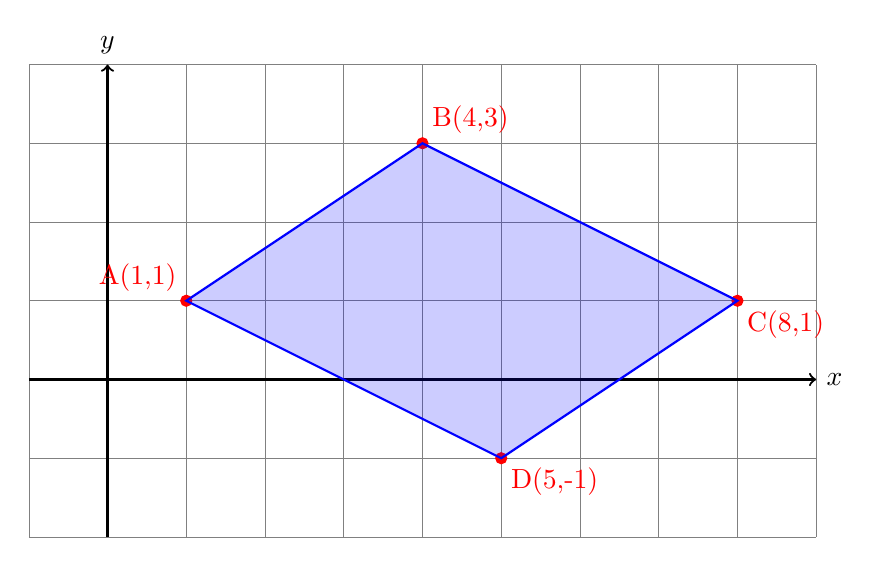
\begin{tikzpicture}
    % Grille de fond
    \draw[step=1cm, gray, very thin] (-1,-2) grid (9,4);

    % Axes
    \draw[thick,->] (-1,0) -- (9,0) node[right] {$x$};
    \draw[thick,->] (0,-2) -- (0,4) node[above] {$y$};

    % Points A, B, C, D
    \filldraw[red] (1,1) circle (2pt) node[above left] {A(1,1)};
    \filldraw[red] (4,3) circle (2pt) node[above right] {B(4,3)};
    \filldraw[red] (8,1) circle (2pt) node[below right] {C(8,1)};
    \filldraw[red] (5,-1) circle (2pt) node[below right] {D(5,-1)};
   % Surlignage du parallélogramme
    \fill[blue, opacity=0.2] (1,1) -- (4,3) -- (8,1) -- (5,-1) -- cycle;

    % Lignes reliant les points
    \draw[thick, blue] (1,1) -- (4,3) -- (8,1) -- (5,-1) -- cycle;

\end{tikzpicture}


\end{center}

On a donc que l'aire = $\begin{pmatrix}
    
\end{pmatrix}$
\end{exemple}


\subparagraph{Aire et application linéaire}
Une application linéaire $T : \mathbb{R}^2 \to \mathbb{R}^2$ transforme les vecteurs $\vec{e}_1$ et $\vec{e}_2$ en deux vecteur u et v. Ainsi $T$ transforme les carré unité de sommets



\begin{theorem}
    Soit $T : \mathbb{R}^2 \to \mathbb{R}^2$  une appliation linéaire représentée par la matrice $A$. Soit $S$ une région du plan alors:
\begin{formule}
    \[Aire(T(S)) = |\det A| \cdot Aire(S)\]
\end{formule}
\end{theorem}
\begin{framedremark}
    L'aire d'un prallélogramme ou le volume d'un parraéélépiède ne dépendent que des vecteurs qui les supportent. L'un des sommets peut être l'origine ou non. L'aire et le volume sont \textbf{invariants par translation}.
\end{framedremark}
\begin{exemple}
    On cherche l'aire de l'ellipse d'équation$\frac{x^2}{a^2} + \frac{y^2}{b^2} = 1$
    \\
    L'application est:
    \[T: \mathbb{R}^2 \to \mathbb{R}^2 \]
    \[\begin{pmatrix}
        x \\ y
    \end{pmatrix} \to \begin{pmatrix}
        ax \\ by
    \end{pmatrix}\]
    La matrice est donc: 
    \[\begin{pmatrix}
        a & 0\\ 0 & b
    \end{pmatrix}\]
    \\
    Le cercle unité $e$ d'équation $x^2 + y^2 ) 1$ est transformé en $\epsilon$ par $T$. Si $(x, y) \in e$:
    \[T\begin{pmatrix}
        x \\ y
    \end{pmatrix} = \begin{pmatrix}
        ax \\ by
    \end{pmatrix} \in \epsilon\] car $\frac{(ax)^2}{a^2} + \frac{(by)^2}{b^2} = x^2 + y^2$
    \\
    Aire($\epsilon$) $= \det \begin{pmatrix}
        a & 0 \\ 0 & b
    \end{pmatrix} \cdot Aire(e) = \pi\cdot a \cdot b$
\end{exemple}





\lecture{12}{2024-10-17}{Générateur}{}


Soit $W$ un sous espace vectoriel $V$.
\begin{itemize}
    \item Le sous espace $W = Vect(v_1, \dots, v_k)$ est le sous espace engendré par les vecteurs $v_1, \dots, v_k$.
    \item Les vecteurs $v_1, \dots, v_k$ sont les générateurs de $W$
    \item L'ensemble $\{v_1, \dots, v_k\}$ forme une \textbf{partie génératrice} de $W$.
\end{itemize}
\begin{exemple}
    Il existe en général plusieurs parties génératrices:
    \[W = Vect\left\{\begin{pmatrix}
        1 \\ 0 \\ 1
    \end{pmatrix}, \begin{pmatrix}
        
    \end{pmatrix}\right\}\]
\end{exemple}
\paragraph{Partie libres}
Soit $W$ un sous-espace vectoriel de $V$.
\begin{itemize}
    \item Les vecteurs $v_1, \dots, v_k$ de $W$ sont linéairement indépendants si la seul combinaison linéaire $\alpha_1v_1 + \cdots + \alpha_kv_k$ qui donne le vecteur nul est la combinaison linéaire triviale:
    \[\alpha_1 = \cdots = \alpha_k = 0\]

    \item On dit que l'ensemble $\{v_1, \dots, v_k\}$ est une \textcolor{red}{partie libre} de $W$.
\end{itemize}


\paragraph{Bases canoniques}

\subparagraph{Le cas de $\mathbb{R}^n$}
La base canonique est 
\begin{formule}

\[
\mathcal{C}an = (\vec{e}_1, \vec{e}_2, \ldots, \vec{e}_n)
\]
\end{formule}
C'est une base car nous avons vu que tout vecteur de \R$^n$ s'écrit comme combinaison linéaire des $\vec{e}_i$.
\\
\subparagraph{Le cas de $P_n$}
La base canonique est 
\begin{formule}
    

\[
\mathcal{C}an = (1, t, t^2, \ldots, t^n)
\]
\end{formule}
Ici aussi tout vecteur de $\mathbb{P}_n$, i.e. tout polynôme de degré $\leq$ n s'écrit comme combinaison linéaire de ces monômes $t^i$, car un tel polynôme est de la forme $a_0\cdot 1 + a_1\cdot t + \dots + a_n\cdot t^n$.
\subparagraph{Le cas de $M_{m \times n}(\mathbb{R})$}
La base canonique est 
\begin{formule}
\[
\mathcal{C}an = (e_{11}, \ldots, e_{1n}, e_{21}, \ldots, e_{m1}, \ldots, e_{mn})
\]
\end{formule}
où $e_{ij}$ est la matrice constituée de zéros, sauf le coefficient $(i, j)$ qui vaut 1. Dans $M_{3\times 2}$(\R), la base canonique est donnée dans cet ordre :
\\
\[e_{11} = \begin{pmatrix}
    1 & 0\\
    0 & 0 \\
    0 & 0
\end{pmatrix}, e_{12} = \begin{pmatrix}
    0 & 1 \\ 0 & 0 \\ 0 & 0
\end{pmatrix}, e_{22} = \begin{pmatrix}
    0 & 0 \\ 1 & 0 \\ 0 & 0
\end{pmatrix} \dots, e_{32} = \begin{pmatrix}
    0 & 0 \\ 0 & 0 \\ 0 & 1
\end{pmatrix} \]

\subparagraph{Exemple}
Soit $W$ le plan dans \R$^3$ donné par l'équation $x + y + z = 0$. L'inconnue $x$ est principale, les inconnues, $y, z$ sont secondaires et seront nos paramètres.
\[x = -y -z\]
Les vecteurs $\vec{b_1} = \begin{pmatrix}
    -1 \\ 1 \\ 0
\end{pmatrix}$ et $\vec{b_2} =  \begin{pmatrix}
    -1 \\ 0  \\1
\end{pmatrix}$ forment une base $\beta = (\vec{b_1}, \vec{b_2}$) de $W$.
\begin{framedremark}
    Il n'y a pas de base canonique dans $W$. Nous avons fait des choix de paramètres, Il y a pas une "\textit{norme}" pour la base canonique ici.
\end{framedremark}
\begin{exemple}
    Si on considère $x, y$ comme inconnues libres, $z$ en principales, alors on trouve une autre base:
    \[c = \begin{pmatrix}
        
    \begin{pmatrix}
        1 \\ 0 \\ -1
    \end{pmatrix}, & \begin{pmatrix}
        0 \\ 1 \\ -1
    \end{pmatrix}\end{pmatrix}\]
\end{exemple}
\subparagraph{Théroème de la base extraite}
Soit $\{v_1, \dots, v_k\}$ une famille de vecteurs qui engendrent $V$.
\begin{theoreme}
    \begin{itemize}
        \item Si l'un des vecteurs $v_i$ est combinaison linéaire des autres, alors la famille obtenue en supprimant $v_i$ engendre encore $V$.
        \item Si $V \neq \{0\}$, il existe une sous-famille de $\{v_1, \dots, v_k\}$ qui forme une base de $V$
    \end{itemize}
\end{theoreme}
\subparagraph{Preuve} \textbf{(A)} pour $i = k$. On suppose que
\begin{formule}
    \[v_k = \alpha_1v_i + \dots + \alpha_{k-1}v_{k-1}\]
\end{formule}
Puisque la famille $\{v_1, \dots, v_k\}$ engendre $V$, tout vecteur $v \in V$ est combinaison linéaire de $v_i$.
\begin{align*}
v &= \beta_1 v_1 + \cdots + \beta_{k-1} v_{k-1} + \beta_k v_k \\
  &= \beta_1 v_1 + \cdots + \beta_{k-1} v_{k-1} + \beta_k (\alpha_1 v_1 + \cdots + \alpha_{k-1} v_{k-1}) \\
  &= (\beta_1 + \beta_k \alpha_1) v_1 + \cdots + (\beta_{k-1} + \beta_k \alpha_{k-1}) v_{k-1}
\end{align*}
Nous avons montré que $v$ est combinaison linéaire de $v_1, \dots, v_{k-1}$.
\\
\textbf{(B)} Si la famille est libre on arrête tout, sinon il suffit de prendre notre point (A) et d'enlever un générateur $v_i$ et en enlevant un denouveau et un autre et un autre... jusqu'à que la famille soit libre. Le processus s'arrête puisque le nombre de vecteur au départ est \textbf{fini}.









\subparagraph{Combinéaisons linéaires d'une base}
Soit $V$ un espace vectoriel et $\mathcal{B} = (e_1 + \dots, e_n)$ une base.
\begin{theoreme}
    Tout vecteur $x$ de $V$ s'écrit de manière unique comme combinaison linéaire $x = x_1e_1 + \dots + x_ne_n$, pour des nombres réels $x_1, \dots, x_n$.
\end{theoreme}
\textbf{Existence} Une base est un \textcolor{red}{système de générateurs}!
\\
\textbf{Unicité} Si $x_1e_1 + \dots + x_ne_n = y_1e_1 + \dots y_ne_n$ alors, 
\[(x_1 - y_1)e_1 + \dots +(x_n - y_n)e_n = 0\]
Une base est \textcolor{red}{libre}, ainsi $x_1 = y_1, \dots, x_n = y_n$
\paragraph{Coordonnées}
\begin{definition}
    Les composantes ou coordonnées d'un vecteur $x$ dans la base $\mathcal{B}$ sont les coefficients réels $x_1, \dots, x_n$ tel que
    \[x = x_1e_1 + \dots + x_ne_n\]
\end{definition}
J'affirme que $
B = \left(
\begin{pmatrix}
1 \\
0 \\
-1
\end{pmatrix},
\begin{pmatrix}
1 \\
-1 \\
0
\end{pmatrix},
\begin{pmatrix}
0 \\
1 \\
1
\end{pmatrix}
\right)
$ est une base de \(\mathbb{R}^3\). En effet, $\begin{pmatrix}
    1 & 1 & 0 \\
    0 & -1 & 1 \\
    -1 & 0 & 1
\end{pmatrix}$ est inversible. Le vecteur $\vec{u} = \begin{pmatrix}
    1 \\ 2 \\ 3
\end{pmatrix}$ de \R$^3$ s'exprime comme combinaison linéaire des $\vec{b}_i$ et on cherche $(\vec{u})_\mathcal{B}$. On doit résoudre :

\[\left ( \begin{array}{ccc|c}
    1 & 1 & 0 & 1 \\
    0 & -1 & 1 & 2 \\
    -1 & 0 & 1 & 3
\end{array} \right) \to \left (\begin{array}{ccc|c}
    1 & 0 & 0 & 0 \\
    0 & 1 & 0 & 1 \\
    0 & 0 & 1 & 3 
\end{array}\right )\]

La solution est :
$(\vec{u})_\mathcal{B} =  \begin{pmatrix}
    0 \\ 1 \\ 3
\end{pmatrix}$ et $(\vec{u})_{\mathcal{C}
an} = \begin{pmatrix}
    1 \\ 2 \\ 3
\end{pmatrix}$
\subparagraph{Comparaison avec \R$^n$}
\begin{definition}
    Une application linéaire bijective et appelée \textcolor{red}{isomorphisme}
\end{definition}
Un isomorphisme permet d'identifier la source et le but de cette application linéaire $T : V \to W$. Les éléments de $V$ et $W$ se correspondent parfaitement, et les opérations de somme et d'action aussi.
\begin{theoreme}
    Soit $V$ une espace vectoriel et $\mathcal{B}$ une base de $n$ vecteurs. \\
    L'application $T : V \to \mathbb{R}^n$ définie par $T(x) = (x)_{\mathcal{B}}$ est un isomorphisme.
\end{theoreme}
\begin{dem}
    Nous devons prouver quatre points, les deux premiers pour montrer que $T$ est linéaire, les deux autres pour établir l'injectivité, et enfin la surjectivité.
    \begin{itemize}
        \item $T(\lambda v) = \lambda T(v)$ pour tout $\lambda \in$ \R et tout $v \in V$;
        \item $T(v + w) = T(v) + T(w)$ pour tous $v, w \in V$;
        \item $T(v) = \vec{0} \implies v = 0$ (critère d'injectivité);
        \item Pour tout $\vec{b} \in$ \R$^n$ il existe $v \in V$ tel que $T(v) = \vec{b}$

    \end{itemize}
    Soit donc $\lambda \in$ \R et $v, w \in V$ que nous écrivons de manière unique! comme $v = x_1e_1 + \dots + x_ne_n$ et $w = y_1e_1 + \dots + y_ne_n$.
\end{dem}
Prouve que le premier point:

\begin{align*}
T(\lambda v) &= T ( \lambda(v_1b_1 + \dots + v_nb_n)) \\
&= T(\lambda v_1 b_1 + \dots + \lambda v_nb_n) \\
&= T\begin{pmatrix}
    \lambda v_1 \\
    .\\\\. \\ \lambda v_n
\end{pmatrix} = \lambda \begin{pmatrix}
    v_1 \\ \\. \\. \\v_n
\end{pmatrix} = \lambda T(v)
\end{align*}

\begin{exemple}
    \begin{itemize}
        \item $T : M_{x\times2}(\mathbb{R}) \to $ \R$^4$ est un isomorphisme. Pour la base canonique $\mathcal{C}an = (e_{11}, e_{12}, e_{21}, e_{22})$, on a:
\[T\begin{pmatrix}
    a & b \\ c & d
\end{pmatrix} = \left ( \begin{pmatrix}
    a & b \\ c & d
\end{pmatrix}\right )_{\mathbf{C}can} = \begin{pmatrix}
    a \\ b \\ c \\ d
\end{pmatrix}\]
        \item $T : \mathbb{P}_3 \to $\R$^4$ est un isomorphisme. Pour la base canonique $\mathcal{C}an = (1, t, t^2, t^3)$ on a
\[T(a + bt + ct^2 + dt^3) = \begin{pmatrix}
    a \\ b \\ c \\ d
\end{pmatrix}\]
\item Soit $W$ le plan dans \R$^3$ donné par l'équation $x + y + z = 0$ et $\mathcal{B}$ la base formée des vecteurs $\vec{b}_1 = \begin{pmatrix}
    -1 \\ 1 \\ 0
\end{pmatrix}$ et $\vec{b}_2 =  \begin{pmatrix}
    -1 \\ 0 \\ 1
\end{pmatrix}$
On a l'application $T : W \to \mathbb{R}^2$
\[w \to \begin{pmatrix}
    a \\ b
\end{pmatrix} \text{ si } w = a\cdot\vec{b_1} + b\cdot\vec{b}_2\]
\end{itemize}

\end{exemple}


\subparagraph{Base et coordonnées}
\begin{definition}[pivots]
    La famille $(p, q, r)$ est une base de $\mathbb{P}^2$ si et seulement si la matrice carrée $A$ a trois pivots. Où $A$ est la matrice d'application avec les vecteurs $(p, q, r)$ fourni dans la base canonique.
\end{definition}

\paragraph{Cardinalité d'une base}
Pour généraliser ce qu'on a dit avant:
\begin{itemize}
    \item $V$ est un espace vectoriel
    \item $\mathcal{B} = (b_1, \dots, b_n)$ une base $V$
    \item $\mathcal{C} = (c_1, \dots, c_m)$ une famille ordonnée de vecteurs de $V$.
\end{itemize}

\begin{theoreme}
    La famille ordonnée de $\mathcal{C}$ est une base de $V$ si et seulement si la matrice $A = ((c_1)_{\mathcal{B}}, \dots, (c_m)_{\mathcal{B}})$ a un pivot dans chaque ligne et chaque colonne.
\end{theoreme}
\begin{framedremark}
    En particulier $A$ est une matrice carrée ($m = n$) et inversible
\end{framedremark}
\begin{theoreme}
    Deux bases de $V$ ont le même nombre d'éléments
\end{theoreme}
\begin{corollaire}
Si $V$ admet une base de $n$ vecteurs, alors une famille $\{v_1, \dots, v_k\}$ de vecteurs de $V$ avec $k > n$ est liée.
\end{corollaire}
\begin{definition}
    Soit $V$ un espacevectoriel et $\mathcal{B} = (e_1, \dots, e_n)$ une base. La \textcolor{red}{dimension} de $V$ est $n$. On note $dim V = n$.
\end{definition}

\begin{itemize}
    \item $dim \mathbb{R}^n = n$
    \item $dim \mathbb{P}_n = n+1$
    \item $M{m\times n}(\mathbb{R}) = mn$
\end{itemize}
\paragraph{La dimension rappel}
\lecture{13}{2024-10-29}{Base, noyau, image}{}
\begin{theoreme}
    Deux bases $V$ de ont le même nombre d'éléments
\end{theoreme}

\begin{definition}
    Soit $V$ un espace vectoriel et $\mathcal{B} = (e_1, \dots, e_n)$ une base. La \textcolor{red}{dimension} de $V$ est $n$. On note $dim V = n$.
\end{definition}
\begin{framedremark}
    On peut prendre par exemple les bases les plus connues:
    \begin{itemize}
        \item $dim $\R$^n = n$
        \item $dim \mathbb{P}_n = n + 1$
        \item $dim M_{m \times n}($\R$) = mn$
    \end{itemize}
\end{framedremark}

\begin{definition}
    Un espace vectoriel $V$ est de dimension nulle si et seulement si $V = \{0\}$.
\end{definition}
0 est un vecteur linéairement dépendant, il ne peut donc faire partie d'aucune base. La convention dite auparavant est : $Vect\{\emptyset\} = \{0\}$. Ainsi l'ensemble vide est une famille livre de générateur de $\{0\}$.

\begin{theoreme}[de la base incomplète]
    Soit $V$ un espace vectoriel de dimension $n$ et $\{e_1, \dots, e_k\}$ une famille libre de veteurs de $V$. Il exciste alors des vecteurs $e_{k+1}, \dots, e_n$ tels que ($e_1, \dots, e_n)$ forme un base de $V$.
\end{theoreme}
\begin{framedremark}
    Attention à ne pas confondre une base et des vecteurs c'est pour ça qu'ici on choisit des parenthèse pour une base et des allocalade pour une famille de vecteurs.
\end{framedremark}

\subparagraph{preuve} So $(e_1, \dots, e_k)$ forme déjà une base de $V$, on s'arrête là.\\
Sinon il existe un veteur $e_{k+1}$ qui n'est pas dans $Vect\{e_1, \dots, e_k\}$. J'affirme que $\{e_1, \dots, e_k, e_{k+1}\}$ est libre.
\\
\begin{itemize}
    \item En effet si $\alpha_1e_1, \cdots + \alpha_ke_k + \alpha_{k+1}e_{k+1} = 0$ alors $\alpha_{k+1} = 0$ car $e_{k+1}$ n'est pas combinaison linéaire des autres $e_j$ par construction.
    \item Ainsi $\alpha_1e_1 + \cdots + \alpha_ke_k  = 0$.
    \item Comme la famille de départ est libre, tous les $\alpha_i$ sont nuls
    \item On peut donc ajouter $e_{k+1}$ à la famille $\{e_1, \dots, e_k\}$
\end{itemize}
On continue ce processus inductif jusqu'à compter $n$ vecteurs


\begin{exemple}
Dans $M_{2 \times 3}(\mathbb{R})$, $dim = 6$ on prend les quatre matrices:
\[A = \begin{pmatrix}
    1 & 0 & 0 \\ 1 & 1 & 0
\end{pmatrix} ,  B = \begin{pmatrix}
    1 & 1 & 0 \\ 0 & 1 & 0
\end{pmatrix}, C  = \begin{pmatrix}
    1 & 0 & 0 \\ 0 & 1 & 0
\end{pmatrix}, D = \begin{pmatrix}
    1 & 0 & 0 \\ 0 & -1 & 0
\end{pmatrix}\]
Si on écrit ces matrices dans la base canonique de $M_{2\times 3}(\mathbb{R}), \mathcal{C}an$ et qu'on créer une matrice avec les lignes de ces vecteurs on a:
\[M = \begin{pmatrix}
    1 & 0 & 0 & 1 & 2 & 0\\
    1 & 1 & 0 & 0 & 1 & 0\\
    1 & 0 & 0 & 0 & 1 & 0 \\
    1 & 0 & 0 & 0 & - 1 & 0 \\
\end{pmatrix} \to \begin{pmatrix}
    1 & 0 & 0 & 0 & 1 & 0\\
    0 & 1 & 0 & 0 & 0 & 0\\
    0 & 0 & 0 & 1 & 0 & 0 \\
    0 & 0 & 0 & 0 & - 2 & 0 \\
\end{pmatrix} \]
On voit ici qu'il y a deux vecteurs be sibt oas des colonnes pivots ($e_{13}, e_{23})$, il ne sont donc pas combinaison linéaire de $A'$ ni de $A$.
\\
Et donc $(A, B, C, D, e_{13}, e_{23})$ est une base de $M_{2\times 3}(\mathbb{R})$.
\begin{framedremark}
    On a rajouter $e_{13}$ et $e_{23}$ car il ne sont pas combinaison linéaire.
\end{framedremark}
\end{exemple}

\paragraph{Deux points de vue sur les bases}
Soit $V$ un espace vetoriel de dimension $n$. Une \textcolor{red}{base} est une famille ordonnée de générateurs libre de $V$. Nous avons vu que toute base est composée du même nombre $n$ de vecteurs.
\\
\textbf{Critères}
\begin{itemize}
    \item Une famille libre $\mathcal{L}$ de $n$ vecteurs forem une base de $V$
    \item une famille génératrice $\mathcal{G}$ de $n$ vecteurs forme une base de $V$.
\end{itemize}
\\

Soit $\mathcal{F}  = \{f_1, \dots, f_k\}$ une famille génératrice de $V$ et $\mathcal{B} = (e_1, \dots, e_n)$ une base de $V$. Pour extraire une base de $\mathcal{F}:$
\begin{itemize}
    \item trouver les composantes des $f_j$ dans la base $\mathcal{B}$
    \item Ecrire la matrice $F$ dont les \textcolor{red}{colonnes} sont les $(f_j)_{\mathcal{B}}$.
    \item Echelonner $F$. (sur les lignes)
    \item Ne garder que les $n$ colonnes pivots de $F$.
    
\end{itemize}

\begin{exemple}
    Extraire de la famille $\{1 - t, -1 + t^2, t^2 - t, 1 + t, t^2 + 1\}$ une base de $\mathbb{P}^2$. On choisit la base canonique de $\mathbb{P}^2$:
    \[(1-t)_{\mathcal{C}an} = \begin{pmatrix}
        1 \\ -1 \\ 0
    \end{pmatrix}, (-1+t^2)_{\mathcal{C}an} = \begin{pmatrix}
        -1 \\ 0 \\ 1
    \end{pmatrix}, \dots \text{et on écrit:}\]
    \[A = \begin{pmatrix}
         1 &-1&0 & 1 & 1 \\
        -1&0&-1&1&0\\
         0&1&1&0&1
    \end{pmatrix} \to \begin{pmatrix}
         1 &-1&0 & 1 & 1 \\
        0&-1&-1&2&1\\
         0&0&0&2&2
    \end{pmatrix}\]
    La prochaine étape après avoir échelonner et de ne garder que les $n$ colonnes pivots de $F$, on voit donc choisir ici $3$ vecteurs qui ont chacun un pivot sur une ligne différente, les colonnes $1, 2, 4$. Ce qui donne:
    \[\mathcal{B} = (1-t, 1+t^2, 1+t)\] \textcolor{red}{Attention!}, on prend les colonnes qui sont les vecteurs et non directement les valeurs trouvées lorsqu'on échelonne. on prend les vecteurs qui se trouvaient sur les colonnes $1, 2, 4$.
\end{exemple}

\paragraph{Comment compléter une base}
Soit $\mathcal{F} = \{f_1, \dots, f_k\}$une famille libre de $V$ dont on a une base $(e_1, \dots, e_n)$. Pour compléter $\mathcal{F}$ en une base:
\begin{itemize}
    \item Trouver les composantes des $f_j$ dans la base $\mathcal{B}$.
    \item Ecrire la matrice $F$ dont les \textcolor{red}{lignes} sont les $(f_j)_{\mathcal{B}}$
    \item Echelonner $F$. (comme d'habitude)
    \item Ajouter les vecteurs $e_i$ pour les valeurs de $i$ qui ne son pas des colonnes pivot.
\end{itemize}

\begin{exemple}
    Compléter la famille $\{\vec{e_2} -\vec{e_1}, \vec{e_3} -\vec{e_1}, \vec{e_4} - \vec{e_1}\}$ en un base de \R$^4$.
    \[A = \begin{pmatrix}
        -1 & 1 & 0 & 0 \\
        -1&0&1 & 0\\
        -1&0&0 & 1
    \end{pmatrix}\to \begin{pmatrix}
        -1 & 0 & 0 & 1 \\
        0&1&0 & -1\\
        0&0&1 & -1
    \end{pmatrix} \]
    On voit qu'il y a pas de pivot sur la dernière colonne.
\end{exemple}


\paragraph{Rappels application linéaires:}
Soit $V$ et $W$ deux espaces vectoriels.
\begin{definition}[application linéaire]
    Une application $T : V \to W$ est \textcolor{red}{linéaire} si
    \begin{enumerate}
        \item $T(u + v) = Tu + Tv$ pour tous $u, v \in V$
        \item $T(\alpha v) = \alpha Tv$ pour tous $v \in V$ et $\alpha \in $\R
    \end{enumerate}
\end{definition}
\begin{exemple}
    \begin{enumerate}
        \item La dérivée $D : \mathcal{C}^\infty(\mathbb{R}) \to \mathcal{C}^\infty(\mathbb{R}) $ des a faire plus tard
    \end{enumerate}

    Contre exemple:
    \\ 
    L'application $C : \mathbb{P}_2 \to \mathbb{P_4}$ définie par 
    \begin{formule}
\begin{center}
    $p \to p^2$
    \end{center}

    \end{formule}
    n'est pas linéaire. En effet on voit par exemple que:
    \[C(2t) = (2t)^2 = 4t^2 \neq 2t^2 = 2C(t)\]
    \begin{framedremark}
        Généralement, les applications linéaires n'aiment pas quand on les met au carrées.
    \end{framedremark}
\end{exemple}


\paragraph{Noyau}
Soit $T: V \to W$ une application linéaire.
\begin{definition}
    Le \textcolor{red}{noyau} de $T$ est le sous-ensemble $Ker T = \{v \in V | Tv = 0\}$.
\end{definition}
Ce qui veut dire que le noyau est le sous-ensemble des vecteurs qui ont pour image le zéro. donc si on prend par exemple les dérivées, on voit que tout les constantes ont la même image qui est 0 donc le noyaux de l'application linéaire des dérivées et le vecteur des constantes.
\begin{exemple}
    Soit $T: \mathbb{R}^2 \to \mathbb{R}^2$ la projection orthogonale sur l'axe $x = y$.
    On voit que c'est la droite $x$ on a donc que:
    \[T(\vec{e_1}) = \begin{pmatrix}
        \frac{1}{2}\\ \frac{1}{2}
    \end{pmatrix}, T(\vec{e_2}) = \begin{pmatrix}
        \frac{1}{2}\\ \frac{1}{2}
    \end{pmatrix}\]
La matrice de T est donnée par:
\[A = \begin{pmatrix}
    \frac{1}{2} & \frac{1}{2} \\
    \frac{1}{2} & \frac{1}{2}
\end{pmatrix}\]
Essayons de trouver le noyau:
\[A\cdot\begin{pmatrix}
    x \\ y
\end{pmatrix} = \begin{pmatrix}
    0 \\ 0
\end{pmatrix}\]
    On a donc fini avec deux équation qui sont:
    \begin{align*}
        \frac{1}{2}x + \frac{1}{2}y  &= 0\\
        \frac{1}{2}x + \frac{1}{2}y &= 0
    \end{align*}
    On peut déjà deviner ici que le noyau ne sera pas l'ensemble vide, on a deux équations identiques (donc une seule) avec deux variables, cela veut dire qu'il restera donc une variable libre:
    \begin{align*}
        y &= y \\
        y &= -x
    \end{align*}
    Ce qui donne : 
    \[Ker T = Vect\begin{pmatrix}
        -1 \\ 1
    \end{pmatrix}\]
    Ce qui si on le voit graphiquement est assez intuitif:
    Prenons la droite $y = -x$ et $y = x$ on a:
\begin{center}
    

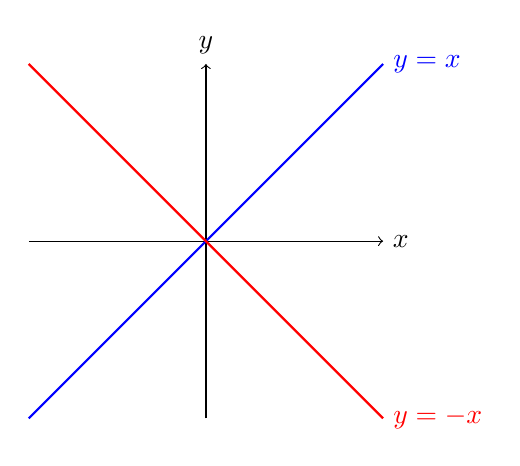
\begin{tikzpicture}[scale=0.75]
    % Axes
    \draw[->] (-3,0) -- (3,0) node[right] {\(x\)};
    \draw[->] (0,-3) -- (0,3) node[above] {\(y\)};

    % Droite y = x
    \draw[blue, thick] (-3,-3) -- (3,3) node[right] {\(y = x\)};

    % Droite y = -x
    \draw[red, thick] (-3,3) -- (3,-3) node[right] {\(y = -x\)};
    
\end{tikzpicture}
\end{center}
On voit que sur chaque point de la droite rouge, si on les ramènes sur la droite bleu (en faisant la projection) il arrive au point $(0, 0)$.
\end{exemple}








\begin{formule
} Cours 14 30/10/2024
\end{formule
}
\paragraph{Le noyau est un sous-espace}
\begin{exemple}
Soit $T : M_{2\times 2}($\R) $\to \mathbb{R}^2$ défini par:
\[T\begin{pmatrix}
    a & b \\ c & d
\end{pmatrix} = \begin{pmatrix}
    c \\ a-d
\end{pmatrix} = \begin{pmatrix}
    0 \\ 0
\end{pmatrix}\]
On vérifie que $T$ est linéaire. Le noyau de $T$ est un sous-ensemble de $M_{2\times 2}($\R). Lequel? C'est le sous-espace:
\[Ker T = \{ \begin{pmatrix}
    a & b \\ 0 & a
\end{pmatrix}|a, b \in \mathbb{R}\}\]
\end{exemple}

\begin{theoreme}
    Soit $T: V \to W$ une application linéaire. Alors $KerT$ est un sous-espace de $V$.
\end{theoreme}

\paragraph{Preuve}
\begin{enumerate}
    \item $0 \in Ker T$ : $T(0) = 0$ car $T$ est linéaire
    \item stabilité de $+$: Si $v, v' \in KerT$, on montre que $v+v' \in KerT$, ce qui donne $0 + 0 = 0$ (les images des éléments du noyau sont tous égaux à 0).
    \item Stabilité de l'action: comme c'est une application linéaire on peut surtout $\alpha$ de l'application, on a donc, $\alpha \cdot 0 = 0$.
\end{enumerate}


\begin{definition}
Soit $T : V \to W$ une application linéaire. Alors $T$ est injective si et seulement si $\ker T = \{0\}$ 
\end{definition}

\begin{exemple}
    On considère $T : \mathbb{R}^4 \to \mathbb{R}^2$ donné par
    \[A = \begin{pmatrix}
        1 & -1 & 1 & -1 \\ 1 & 1 & 1 & 1
    \end{pmatrix}\]
    On a donc que 
    \[Ker T = Ker A = \{\vec{v}\in \mathbb{R}^4| A \cdot \vec{v}= \vec{0}\}\]
    est la solution générale S du système homogène donné par $A$. Si on échelonne la matrice on obtient:
    \[\begin{pmatrix}
        1 & -1 & 0 & 0 \\ 0 & 0 & 1 & -1
    \end{pmatrix}\]
    On en vient à :
    \[S = Ker A = Vect \{ \begin{pmatrix}
        1 \\ 1 \\ 0 \\ 0
    \end{pmatrix}, \begin{pmatrix}
        0 \\ 0 \\ 1 \\ 1
    \end{pmatrix}\}\]
    Les deux vecteurs ici forment une base de $Ker A$.
    \\
    Juste pour expliquer comme on passe de la matrice à vect, on peut par exemple remettre en système d'équation classique du genre:
    \begin{align*}
        x -y + 0 + 0 &= 0\\
        0 + 0 + z - w &= 0
    \end{align*}
    On voit qu'il y aura deux variables libres, et donc:
    \begin{align*}
        x &= x \\
        y &= x\\
        z &= z\\
        w &= z
    \end{align*}
    Voila d'où vient les deux vecteurs, un en fonction de $x$ et l'autre en fonction de $z$.
\end{exemple}

\begin{definition}
    L'\textcolor{red}{image} d'une application linéaire $T : V \to W$ est le sous-ensemble $Im T = \{w \in W| \text{il existe } v \in V $ tel que $Tv = w\}$
\end{definition}
\begin{framedremark}
    Le concept d'image généralise la notion du sous-espace $Col A$ engendré par les colonnes d'une matrice A.
\end{framedremark}

\begin{theoreme}
    Soit $T : V \to W$ une application linéaire. Alors $Im T$ est un sous espace de $W$.
\end{theoreme}
\paragraph{Preuve}
On voit d'abord que $0 = T(0)$ appartient à l'image. Il reste à montrer la stabilité de la somme et de l'action. Traitons le cas de la somme. Soient donc $w, w'$ deux vecteurs de $Im T$. Nous devons montrer que $w + w'$ aussi appartient à $Im T$.
\\
On sait que $w, w' \in ImT$, donc il existe $v, v' \in V \text{tq} T(v) = w $ et $T(v') = w'$.\\
On choisit $v_2 = v + v'$ et on calcule par linéarité de $T$ : \[T(v_2) = T(v + v') = T(v) + T(v') = w + w'\]
Donc, $w + w' \in Im T$  (on a le droit de faire tout ça parce que $T$ est une application linéaire.
\\
Pour ce qui est de l'action, on peut juste faire le même procédé et grâce au faite que $T$ est une application linéaire, ça marchera aussi.


\begin{framedremark}
    Soit $T : V \to W$ une application linéaire. Alors $Ker T$ est un sous-espace de $V$, mais $Im T$ est un sous-espace de $W$. (Attention à où vit ces ensembles)
\end{framedremark}

\begin{exemple}
    Soit $D : \mathbb{P}_3 \to \mathbb{P}_3$ la dérivation, $D(p) = p'$.
    \begin{itemize}
        \item $Ker D = \{p \in \mathbb{P}_3 | p' = 0\} = \{a \in \mathbb{P}_3 | a \in $ \R $\}$ (le polynôme constants \[= Vect\{1\}\]

        \item $Im D = \{q \in \mathbb{P}_3 | \exists p \in \mathbb{P}_3$ avec $D(p)  = q\}$
\[= Vect\{1, t, t^2\} \subset \mathbb{P}_3\]
Pour expliquer un peu, on sait que tout les polynômes qui ont que des constantes vont sur $0$ donc on prend le vecteur des constantes qui lui nous ramène de toutes les constantes à $0$.\\
De l'autre côté, l'image reprends tout ce qui arrive de l'autre côté, on voit qu'il y a pas $t^3$ dans l'image, quand on dérive un polynôme, il devient de degrés $2$. Donc la base de l'image va, "\textit{avec le noyau}" et $t^2$

    \end{itemize}
\end{exemple}

\paragraph{Méthode de calcul}
Soit $T : \mathbb{R}^n \to \mathbb{R}^m$ une application linéaire, représentée par une matrice $A \in M_{m\times n}(\mathbb{R})$.
\begin{itemize}
    \item Pour calculer le \textcolor{red}{noyau} de $T$ on échelonne et réduit la matrice $A$ selon les \textcolor{red}{lignes}.
    \item Pour calculer l'\textcolor{blue}{image} de $T$ on ne garde que les \textcolor{blue}{colonnes-pivotss}. Si nécessaire on échelonne et réduit $A$ selon les \textcolor{blue}{colonnes}.
\end{itemize}

\begin{framedremark}{espace-colonne}
    On appelle parfois \textcolor{red}{espace-colonne} le sous-espcae $ColA$ engendré par les colonnes de $A$. Il s'agit donc de $Im A$
\end{framedremark}
\paragraph{explication de pourquoi ça marche}
Soit $A \in M_{m\times n}(\mathbb{R})$ et $B$ la matrice échelonnée associée ($B$ est juste la matrice échelonnée).
\\
SI une colonne n'a pas de pivot, le système $A\vec{x} = \vec{0} $ a une infinitén de solutions (les mêmes que $B\vec{x} = \vec{0}$), on peut écrire
\[x_1\vec{a}_1 + \dots + x_n\vec{a}_n = \vec{0}\]


\begin{framedremark}
    Les colonnes sans pivot sont combinaison linéaire des autres colonnes.\\ Les colonnes de $A$ vérifient les mêmes relations de dépendance linéaire que celles de $B$
\end{framedremark}
On peut donc enlever une telle colonne pour engendrer $ColA = ImA$. Les k colonnes-pivot restantes de $A$ sont libres puisque la matrice $m\times k$ formée de ces k colonnes a $k$ pivots.

\begin{exemple}
    On donnt une application linéaire donnée par $A$ tel que:
    \[A = \begin{pmatrix}
        1 & 0 & 0 & -1\\
        -1 & 1 & 0 & 0\\
        0 & -1 & 1 & 0 \\
        0 & 0 & -1 & 1
    \end{pmatrix} \to \begin{pmatrix}
         1 & 0 & 0 & -1\\
        0 & 1 & 0 & -1\\
        0 & 0 & 1 & -1 \\
        0 & 0 & 0 & 0
    \end{pmatrix}\]
    On voit qu'il y a une colonne sans pivot, donc le noyau a qu'une seule variable libre et donc comme on l'avait fait auparavant, on fixe le dernier l'élément, et on voit aussi que chaque $x_1, x_2, x_3$ sont égaux à $1$ ($1 -1  = 0 \to 1 = 1)$ on trouve que:
    \[Ker A = Vect\{\begin{pmatrix}
        1 \\ 1 \\1 \\1 \\
    \end{pmatrix}\}\]
    
\end{exemple}

\paragraph{Rappel critère d'injéctivité (encore)}
Le critère d'injectivité d'une application linéaire permet de ramener la démonstration de l'injectivité au calcul du noyau. Le noyau mesure donc le \textcolor{red}{défaut d'injectivité}.
\begin{theoreme}
    Une application linéaire $T: V \to W$ est injective si et seulement si $Ker T = \{0\}$ 
\end{theoreme}
\paragraph{Espaces-lignes: $LgnA$}
Soit $A$ et $B$ deux matrices de taille $m\times n$ On note $A  \textasciitilde B$ quand elles sont équivalentes selon les lignes.
\begin{theoreme}
    Si $A \textasciitilde B$ alors les lignes de $A$ et $B$ engendrent le même sous-espace de $\mathbb{R}^n$.   
\end{theoreme}
\textbf{Pourquoi?} Les opération élémentaires produisent de nouvelles lignes qui sont cominaison linéaires des précédentes.
\begin{theoreme}
    Les lignes d'une forme échelonnée de $A$ forment une base du sous-espace engendré par les lignes de $A$.
\end{theoreme}
\textbf{Pourquoi?} Aucune ligne non nulle de la forme échelonnée ne peut être combinaison linéaire des autres (à cause de son pivot)

\paragraph{Espaces-colonnes: $ColA$}
Soit $A$ une matrice de taille $m \times n$.
\begin{theoreme}
    Les colonnes pivots de $A$ forment une base de $ColA = Im A$.
\end{theoreme}

\lecture{15}{2024-05-11}{Théroème du rang}{}
\begin{parag}
    

\begin{subparag}{remarque importante}
Soit $A$ une matrice de taille $m \times n$.
\begin{theoreme}

    $dim ColA = dim\; LgnA$

\end{theoreme}
\begin{itemize}
    \item Le nombre de lignes linéairement indépendantes est égal au nombre de lignes contenant un pivot.
    \item Le nombre de colonnes linéairement indépendantes est égal au nombre de colonnes contenant un pivot.
    \item En résumé, $dim\; ColA = dim\; LgnA$ car les deux dimensions coïncident avec le nombre de pivots.

\end{itemize}
    
\end{subparag}


\begin{subparag}{exemple}

Le cas d'une matrice $2\times 2$.
Soit $A =  \begin{pmatrix}
    0 & 0 \\ 0 & 0
\end{pmatrix}$, alors $dim\; LgnA = 0 = dim \; ColA$.\\
Supposons que $A \neq 0$, alors $A = \begin{pmatrix}
    a & b \\ c & d
\end{pmatrix}$. Si les deux colonnes sont proportionelles, $dim\; ColA = 1$  On peut supposer que $\begin{pmatrix}
    b \\ d
\end{pmatrix} = \begin{pmatrix}
    \lambda a \\ \lambda c
\end{pmatrix}$ pour une $\lambda \in $\R. 
\[A = \begin{pmatrix}
    a & \lambda a \\ c & \lambda c
\end{pmatrix}\]
\textbf{Premier cas:} $a = 0$, aussi $\lambda a = 0$ et comme $A \neq 0$, $dim \; LgnA = 1$ ca la $2^e$ ligne est non nulle.
\\
\textbf{deuxième cas} $a \neq 0$ $\begin{pmatrix}
    a & \lambda a \\ c & \lambda c
\end{pmatrix}  $ a deux lignes proportionnelles car $\left(c \; \lambda c\right) = \frac{c}{a}\left(a \; \lambda a\right)$. Ici aussi $dim \; LgnA = 1$.
    
\end{subparag}

\end{parag}

\begin{parag}{Le Théorème du rang}
    



\paragraph{A faire plus tard parce que je sais pas}
    On se ramène au cas d'une application linéaire $R^n \to R^m$, représentée par $A \in M_{m\times n}\left(\mathbb{R} \right)$.
    \begin{enumerate}
        \item On choisit une base $\mathcal{B} = \left(e_1, \dots, e_n\right)$ de $V$
        \item On considère la composition suivante
 \item     \end{enumerate}


\begin{theoreme}{théorème du rang}
    
        \[rangT + dim\; KerT  = dimV\]
    
\end{theoreme}
\begin{itemize}
    \item Grâce aux coordonnées on identifire $V$ avec \R$^n$ et W avec \R$^m$.
    \item Ainsi on identifire $T$ avec une application linéaire $S: \mathbb{n} \to \mathbb{R}^m$.
    \item Celle-ci est donnée par la multiplication matricielle \[\vec{x} \to A\vec{x} = S\left(\vec{x}\right)\]
    \item $dim \; KerA = $ nombre de colonnes sans pivot
    \item $dim \; ImA = \text{rang}A = $ nombre de colonnes-pivot
    \item  nombre de colonnes-pivot $+$ colonnes sans pivot $= n$.
\end{itemize}

\begin{subparag}{Idée de la preuve}
    

Si $dim V = n$, $dim \; KerT = k \leq n$ car $KerT \subset V$. On choisit une base $\left(e_1, \dots, e_k\right)$ de $KerT$. Grâce au Théorème de la base complétée, il existe $\left(e_{k+1}, \dots, e_n\right)$  tel que $\left(e_1, \dots, e_k, e_{k+1}, \dots, e_n\right) $ est une base de V. 
\\
Alors $\{T\left(e_1\right), \dots, T\left(e_k\right), T\left(e_{k+1}\right), \dots, T\left(e_n\right)\}$ engendrent $ImT$.
\\
Donc $\{T\left(e_{k+1}, \dots, T\left(e_n\right)\right)\}$ engendrent $ImT$.
\\
Mais T | $Vect\{e_{k+1}, \dots, e_n\}$ est injective car $KerT \cap U = \{0\}$.
Donc $T\left(e_{k+1}\right), \dots, T\left(e_n\right)$ sont libres, donc forment une base. Conclusion \[RangT  = n - k\]
\end{subparag}


\begin{definition}
Soit $T : V \to W$ une application linéaire entre espaces vectoriels de dimension finies.
\\
Le \textcolor{red}{rang} de $T$ est la dimension de l'image de $T$ : 
\[rang T = dim \; ImT\]
\end{definition}

\begin{definition}
Soit $A$ une matrice $m \times n$, représentant une application linéaire.
\\
    Le \textcolor{red}{rang} de $A$ est la dimension de l0image de $A: $ $rangA = dim\; ImA$.
\end{definition}
\begin{theoreme}{théorème du rang}
    
        \[rangT + dim\; KerT  = dimV\]
    
\end{theoreme}
    \begin{subparag}{Exemple}
        Considérons l'application linéaire $T: \mathbb{P}_2 \to $ \R$^2$ définie par:
        \[T\left(p\right) = \begin{pmatrix}
            p\left(0\right) \\ p\left(1\right)
        \end{pmatrix}\]
        Pour tout polynôme $p$ de degrès $\leq 2$.
        \\
        Nous allons 
        \begin{itemize}
            \item Calculer le noyau
            \item en déduire la dimension de l'image grâce au théorème du rang, et
            \item interpréter ce résultat pour conclure que deux zéros d'une fonction polynomiale de degrès $\leq 2$ déterminent le polynôme en question à un facteur près.
        \end{itemize}

        \begin{align*}
        Ker T &= \{p \in \mathbb{P}_2 | p\left(0\right) = 0 = p\left(1\right)\}\\
            &= \{p \in \mathbb{P}_2 | p\left(t\right) = a\cdot t\cdot \left(t - 1\right) \text{ , pour un } a \in \mathbb{R}\} \\
            &= Vect\{\left(t-1\right)\} \text{ de dimension 1.}
        \end{align*}
        Par le théorème du rang, $rang T + dim\;KerT = 3$ donc $rang T = 2 = dim \mathbb{R}^2$.
        \\
        L'interprétation suit: si $p\left(t\right)$ s'annule en $0$ et en $1$, alors $p\left(t\right) = a \cdot t \cdot \left(t- 1\right)$ pour $a \in $ \R.
    \end{subparag}
\end{parag}
 \begin{parag}{Critère d'inversibilité}
     Soit $A$ une matrice carrée de taille $n\times n $. Alors les conditions suivantes sont équivalentes : 
     \begin{enumerate}
         \item La matrice $A$ est inversible
         \item les colonnes de $A$ forment une base de $\mathbb{R}^n$.
         \item $ImA = \mathbb{R}^n$ \hspace{5cm} $A$ est surjective
         \item $dim \; Im A = n$.
         \item $rang\; A = n$
         \item $Ker\;A = \{0\}$ \hspace{4.75cm} $A$ est injective
         \item $dim\; Ker\; A = 0$.
     \end{enumerate}
     \begin{subparag}{Exemple}
         Pour quelles valeurs du paramètre réel $a$ la matrice $A$ suivante est-elle inversible?
         \[\begin{pmatrix}
             a & 1 & 1 & 1\\
             1 & a & 1 & 1\\
             1 & 1 & a & 1\\
             1 & 1 & 1 & a
         \end{pmatrix} \to \begin{pmatrix}
            1 & 1 & 1 & a\\
             0 & a-1 & 0 & 1-a\\
             0 & 0 & a-1 & 1-a\\
             0 & 1-a & 1-a & 1-a^
             
         \end{pmatrix}\]
         (les opérations sont $L_1 - L-4$, $L-2 - L_1'$, $L_3  L_1'$, $L_4 - a\cdot L_1'$)
         Si $a - 1 = 0$ alors $a = 1$ donc:
         \\
         $rang\; A = 1$, $dim \; Ker A = 3$
         \\
         Si $a \neq 1$, on peut diviser chaque ligne par $a-1$, on obtient alors:
 \[\begin{pmatrix}
            1 & 1 & 1 & a\\
             0 & 1 & 0 & -1\\
             0 & 0 & a-1 & -1\\
             0 & 1 & 1 & 1 + a
             
         \end{pmatrix} \to \begin{pmatrix}
            1 & 1 & 1 & a\\
             0 & 1 & 0 & -1\\
             0 & 0 & 1 & -1\\
             0 & 0 & 0 & a + 3
             
         \end{pmatrix}\]
         Les opération ici pour passer à la deuxième matrice sont ($L_3 - L_2 - L_3$) + $+$
     \end{subparag}
 \end{parag}

 \begin{parag}{Une application linéaire}
     Soit $W$ le sous-espace vectoriel de $M_{2\times2}\left(\mathbb{R}\right)$ des matrices triangulaires supérieures.
     \\
     En fait $W = Vect\{e_{11}, e_{12}, e_{22}$ et $\mathcal{B} = (e_{11}, e_{12}, e_{22})$ est une base de $W$.
     \\
     On considère $T : \mathbb{P}_2 \to W$ l'application linéaire définie par
     \[T\left(p\right) = \begin{pmatrix}
         p\left(1\right) & p\left(-1\right) \\
         0 & p\left(2\right)
     \end{pmatrix}\]
     En choisissant la base canonique $\mathcal{C}an = \left(1, t, t^2\right)$, on identifie $\mathbb{P}_2$ avec \R$^3$ et en choisissant la base ci-dessus de $W$ on identifie $W$ avec \R$^3$ également. Ce qui nous donne:
     \[\begin{pmatrix}
         1 \\ 0 \\ 0
     \end{pmatrix} = \vec{e}_1 = \left(1\right)_{\mathcal{C}an} \text{et} 1 \to \begin{pmatrix}
         1 & 1 \\ 0 & 1
     \end{pmatrix} = W_1 \text{et} \left(W_1\right)_{\mathcal{B}} = \begin{pmatrix}
         1 \\ 1 \\ 1
     \end{pmatrix}\]
     \[\begin{pmatrix}
         0 \\ 1 \\ 0
     \end{pmatrix} = \vec{e}_2 = \left(t\right)_{\mathcal{C}an} \text{et} t \to \begin{pmatrix}
         1 & -1 \\ 0 & 2
     \end{pmatrix} = W_1 \text{et} \left(W_2\right)_{\mathcal{B}} = \begin{pmatrix}
         1 \\ -1 \\ 2
     \end{pmatrix}\]
     \[\begin{pmatrix}
         0 \\ 0 \\ 1
     \end{pmatrix} = \vec{e}_3 = \left(t^2\right)_{\mathcal{C}an} \text{et} t^2 \to \begin{pmatrix}
         1 & 1 \\ 0 & 4
     \end{pmatrix} = W_3 \text{et} \left(W_3\right)_{\mathcal{B}} = \begin{pmatrix}
         1 \\ 1 \\ 4
     \end{pmatrix}\]
     \begin{subparag}{remarque}
         En gros on n'a juste "\textit{skip}" $a_{21}$ parce qu'il valait tout le temps $0$. Mais On aurait pu dire que l'ensemble $W$ est un sous-ensemble de $\mathbb{R}^4$ tel que $W \subset \mathbb{R}^4$.
     \end{subparag}
 \end{parag}

 \begin{parag}{Résumé}
     Le théroème du rang peut nous permettre de faire de grand raccourci lors de choix multiple.
     \begin{itemize}
         \item Le rang d'une matrice $A$ de taille $n \times m$ ne peut pas dépasser $n$.
         \[Rang  A + dim\; KerA = n\]
         \item Pour rappel, si on prend une application $A :$ $V \to W$ on a que $Ker A$ est dans $V$ et que $Im A$ est dans $W$.                               
     \end{itemize}
 \end{parag}
\lecture{18}{2024-11-12}{Changement de base}{}

\begin{parag}{Rappels: changement de base}
    Soit $V$ un espace vectoriel de dimension $n$:
    \begin{enumerate}
        \item Soit $\mathcal{B} = (e_1, \dots, e_n)$ une base. On peut alors écrire un vecteur $x \in V$ en \textcolor{red}{coorodnnées} $(x)_\bmath$, où $x = e_1x_1 + \cdots + e_nx_n$.
        \item Soit $\cmath = (f_1, \dots, f_n)$ une autre base. On peut alors écrire un vecteur $x \in V$ en \textcolor{red}{coordonnées} $(x)_\cmath$
        \item Pour passer de $(x)_\bmath$ à $(x)_\cmath$, on utilise la matrice de changement de base $P = (Id)_\bmath^\cmath$ donc les colonnes sont $(e_i)_\cmath$.
        \\
        Alors
        \item La matrice de changement de base inverse $Q = (id)_\cmath^\bmath = P^{-1}$
    \end{enumerate}



    \begin{subparag}{Exemple}
        On travaille dans l'espace vectoriel $W$ des matrices symétriue de taille $2 \tims 2$ (tel que $A = A^t$). Ainsi:
        \[W = \left\{ \begin{pmatrix}
            a & b \\ b & c
        \end{pmatrix}| a, b, c \in \mathbb{R} \right\}\]
        On considère deux base $\bmath = (B_1, B_2, B_3)$ et $\cmath = (C_+, C_2, C_3)$:
        \begin{align*}
            \bmath &= \left(\begin{pmatrix}
                1 & 0 \\ 0 & 0
            \end{pmatrix}, \begin{pmatrix}
                0 & 1 \\ 1 & 0
            \end{pmatrix}, \begin{pmatrix}
                0 & 0 \\ 0 & 1
            \end{pmatrix}\textbf{}\right) \\
            \cmath &= \left(\begin{pmatrix}
                1 & 0 \\0 & 1
            \end{pmatrix}, \begin{pmatrix}
                -1 & 0 \\ 0 & 1
            \end{pmatrix}, \begin{pmatrix}
                0 & 1 \\ 1 & 0
            \end{pmatrix}\right)
        \end{align*}
        \[C_1 = B_1 + B_3, C_2 = -B_1 +B_3 , C_3 = B_2 \]
        Si on exprime donc les colonnes de $C$ en fonction de $\bmath$ on a:
        \[\left((C_1)_B (C_2)_B (C_3)_B \right) = \begin{pmatrix}
            1 & -1 & 0 \\
            0 & 0 & 1\\
            1 & 1 & 0
        \end{pmatrix} = (Id)_\cmath^\bmath = P\]
        On a aussi l'info que $(Id)_\bmath^\cmath = P^{-1}$ qui se calcule avec la méthode de Gauss:
        \[\begin{pmatrix}
            1 & 1 & 0 & | & 1  & 0 & 0\\
            0 & 0 & 1 & | & 0 & 1 & 0 \\
            1 & 1 & 0 & | & 0 & 0 & 1
        \end{pmatrix}\]
    
    \end{subparag}
\end{parag}


\begin{parag}{Double changement de base}
    Soient $\bmath, \cmath$ et $\mathcal{D}$ trois base de $V$.
    \begin{formule}
        \[(Id)_\cmath^{\mathcal{D}}(Id)_\bmath^\cmath = (Id)_\bmath^{\mathcal{D}}\]
    \end{formule}
    \begin{subparag}{Preuve}
        La composition $(V, \bmath) \to (V, \cmath) \to (V, \mathcal{D})$ est l'identité. La multiplication matricielle correspond à la composition.
    \end{subparag}
\end{parag}

\begin{parag}{Diagonalistion}
    Soit $T: V \to V$ une application linéaire
    \begin{subparag}{Objectif}
        Trouver une base $\bmath$ de $V$ telle que $(T)_\bmath^\bmath$ soit facilement compréhensible
    \end{subparag}
    \begin{subparag}{exemple}
        Soit $f : \mathbb{R}^3 \to \mathbb{R}^3$ l'application linare donnée par:
        \[f\begin{pmatrix}
            x \\ y \\ z
        \end{pmatrix} = \begin{pmatrix}
            -y + z \\ -3x -2y + 3z\\
            -2x -2y + 3z
        \end{pmatrix}\]

        Alors:
        \[A = (f)_{\cmath an} ^{\cmath an} = \begin{pmatrix}
            0 & -1 & 1\\
            -3 & -2 & 3\\
            -2 & -2 & 3
        \end{pmatrix} \]
        On voit ici que certains vecteur sont \textcolor{red}{fixés} par $f$ alors que d'autres sont \textcolor{red}{renversés}.\\
        Autrement dit:
        \begin{enumerate}
            \item Il existe des vecteurs $\vec{x} \in \mathbb{R}^3$ tel que $A\vec{x} = \vec{x}$
            \item Il existe des vecteurs $\vec{x} \in \mathbb{R}^3$ tel que $A\vec{x} = -\vec{x}$
        \end{enumerate}
        

    \begin{enumerate}
        \item On choisit $\vec{x} \in \mathbb{R}^3$ tel que $f(\vec{x}) = \vec{x} \Leftrightarrow A\vec{x} = \vec{x} \Leftrightarrow A\vec{x} = I_b \vec{x}$
        \\
        \[(A - I_b)\vec{x} = \vec{0} \Leftrightarrow \vec{x} \in \ker (A - I_b)\]
        Calculons ce noyau:
        \[(A - I_b) = \begin{pmatrix}
            -1 & -1 & 1 \\
            -3  & -3 & 3 \\
            -2  & -2 & 2
        \end{pmatrix} \to \begin{pmatrix}
            1 & 1 & -1 \\
            0 & 0 & 0 \\
            0 & 0 & 0 
        \end{pmatrix}\]
    \item On chercher $\vec{x} \in \mathbb{R}^3$ tel que $f(\vec{x}) = -\vec{x} \Leftrightarrow A\vec{x} = -\vec{x} = -I_b\cdot\vec{x} \Leftrightarrow A\vec{x} + I_b\vec{x} = \vec{0} \Leftrightarrow (A + I_b)\vec{x} = 0 \Leftrightarrow \vec{x} \in \ker (A + I_b)$

    On chercher donc ce noyau:
\[A + I_3 = \begin{pmatrix}
    1 & -1 & 1\\
    -3 & -1 & 3\\
    -2 & -2 & 4
\end{pmatrix} \to \begin{pmatrix}
    1 & 0 & -\frac{1}{2}\\
    0 & 1 & -\frac{3}{2}\\
    0 & 0 & 0
\end{pmatrix}\]

Donc, Ker$(A + I_3)$ est la droite $D = Vect\left\{ \begin{pmatrix}
    \frac{1}{2}\\ \frac{3}{2} \\ 1
\end{pmatrix}\right\} =  Vect \left\{\begin{pmatrix}
    1 \\ 3 \\ 2
\end{pmatrix}\right\} = Vect \{b_3\}$
    \item Conclusion, Au final on a trouvé trois vecteurs linéairement indépendant (à verifier dans le prochain cours) on a $3$ vecteur qui forme une base;
    \[\bmath = \left(\vec{b_1}, \vec{b_2}, \vec{b_3} \right) \text{ dans } \mathbb{R}^3\]
    On a vu que $f(\vec{b}_1) = \vec{b_1}$, $f(\vec{b_2})= \vec{b_2}$, $f(\vec{b_3}) = -\vec{b_3}$\\
    \[(f)_{\cmath an}^{\cmath an} = A, (f)_\bmath^\bmath = \begin{pmatrix}
        1 & 0 & 0 \\
        0 & 1 & 0 \\
        0 & 0 & -1
    \end{pmatrix}\]
    $f$ est la symmétrie qui fixe $W$ dans la direction $D$.
    \end{enumerate}
    \\
    La matrice de $f$ dans la base nouvelle $\bmath$ est \textcolor{red}{diagonale}!
    \begin{enumerate}
        \item Elle est plus parlante géométriquement
        \item Elle est plus facile à manipuler algébriquement, par exemple  pour calculer ses puissances.
    \end{enumerate}
    \end{subparag}
    \begin{subparag}{Remarque personnelle}
        Juste pour que ce soit clair de comment on a trouver la droite on a juste "\textit{reécris}" en mode système et on arrive a trouver donc que un système d'équation qui est une droite.\\
        On verra plus tard ici que ces vecteurs sont en fait les vecteurs propres.
    \end{subparag}
\end{parag}


\begin{parag}{Valeurs propres et vecteurs propres}
Soit $A$ une matrice carrée de taille $n \times n$
    \begin{definition}
        Un vecteur non nul $\vec{x}$ de \R$^n$ est un \textcolor{red}{vecteur propre} de $A$ s'il exsite un nombre $\lambda$ tel que $A\vec{x} = \lambda \vec{x}$. On appelle alors $\lambda$ une \textcolor{red}{valeur propre} de $A$. L'\textcolor{red}{espace propre} $E_\lambda$ est formé de TOUS les vecteurs $\vec{x}$ tels que $A\vec{x} = \lambda\vec{x}$
    \end{definition}
    \begin{subparag}{ATTENTION}
        Pour tout $\lambda \in \mathbb{R}$ on a $A\vec{0} = \lambda \vec{0}$. Il est crucial de demander que $\vec{x}$ soit non nul! Une baleur propre est une dentrée rare! Par contre $\vec{0} \in E_\lambda$.
    \end{subparag}

    \begin{definition}
        Soit $T : V \to V$ une application linéaire. Un vecteur non nul $x \in V$ est un vecteur propre de $T$ si $T(x) = \lambda x$
    \end{definition}

    \begin{subparag}{Comparaison}
        Soit $V$ un espace vectoriel et $\bmath$ une base. Soit $T: V \to V$ une application linéaire.
        \\
        Soit $A = (T)_\bmath^\bmath$ la matrice $T$ dans la base $\bmath$

    \end{subparag}


    \begin{subparag}{Propostion}
        Une vectuer $x$ est un vecteur propore de $T$ pour la valeur propre $\lambda$ si et seulement si $(x)_\bmath$ est un vecteur propre de $A$ pour la même valeur propre $\lambda$.
        \end{subparag}
    \begin{subparag}{Preuve}
        \[A(x)_\bmath = (T)_\bmath^\bmath(x)_\bmath = (T(x))_\bmath\]
        Ainsi $T(x) = \lambda x$ si et seulement si $A(x)_\bmath = \lambda(x)\bmath$
    \end{subparag}

    \begin{subparag}{Exemple}
        Soit $T : \mathbb{P_1} \to \mathbb{P_1}$ l'application linéaire définie par : 
        \[T(a + bt) = -a + 3b + (2a + 4b)t\]
        Si on prend comme base $\cmath an = \{1, t\}$, on a
        \begin{align*}
            T(1) &= -1 + 2t\\
            T(t) &= 3 + 4t
        \end{align*}
        Ce qui donne comme matrice:
        \[(T)_{\cmath an}^{\cmath an} = \begin{pmatrix}
            -1  & 3 \\ 2 &  4
        \end{pmatrix} = A\]
        On observe, avec un peu de change que:
        \[A + 2I_2 = \begin{pmatrix}
            1 & 3 \\ 2 & 6
        \end{pmatrix} \text{ est de rang }1\]
        $A + 2I_2$ a un noyau non nul, de dim $1$ (Théorème du rang) donné par $Vect\left\{ \begin{pmatrix}
            -3 \\ 1
        \end{pmatrix}\right\}$\\
        Ainsi, $\begin{pmatrix}
            -3 \\ 1
        \end{pmatrix}$ est un vecteur propre de $A$ $\left(A\begin{pmatrix}
            -3 \\ 1
        \end{pmatrix} = -2 \cdot\begin{pmatrix}
            -3 \\ 1
        \end{pmatrix}\right)$\\
        $-3 + t$ est bien un vecteur propre de $T$.\\
        Essayons de voir ce qui se passe avec la nouvelle base:
        \[\bmath = \{-3 + t, t\} = \{p_1, p_2\} \text{ de } \mathbb{P_1}\]
        \[T(p_1= -2P_1 \; \; \; \hspace{1cm} T(t) = 3 + 4t = -(-3 + t) + 5\cdot t = -1 p_1 + 5p_2\]
        \[(T)_\bmath^\bmath = \begin{pmatrix}
            -2 & -1 \\ 0 & 5
        \end{pmatrix} = B \hspace{3cm} \text{ Pas encore diagonale, mais triangulaire}\]
        Cela noud aise à voir que 5 est eaussi une valeur propre car Ker$(B - 5I_2) = Ker \begin{pmatrix}
            -7 & -1 \\ 0 & 0
        \end{pmatrix} = Vect\left\{\begin{pmatrix}
            -1 \\ +7
        \end{pmatrix}\right\}$\\
        Ainsi, $\begin{pmatrix}
            -1 \\ 7
        \end{pmatrix}$ est un vecteur propre de $B$, la matrice de $T$ dans la base $\bmath$, donc $-1\cdot p_1$ + 7\cdot p_2 A faire j'ai pas\\
        On choisit une nouvelle base $\cmath = (-3 + t, 1 + 2t) = (q_1, q_2)$.\\
        \begin{align*}
            T(q_1) &= -2\cdot q_1\\
            T(q_2) &= 5\cdot q_2
        \end{align*}
        Ce qui implique que:
        \[(T)_\cmath^\cmath ) \begin{pmatrix}
            -2 & 0 \\ 0 & 5
        \end{pmatrix}\]
    \end{subparag}
    \end{parag}     

    \begin{parag}{Valeur propre et noyau}
        \begin{subparag}{Proposition}
            Un nombre $\lambda$ est valeur propre de $A$ si et seulement si le noyau de $A - \lambda I_n$ est non nul.
        \end{subparag}
        
        \begin{subparag}{Preuve}
            Si $\lambda$ est valeur propre de $A$, il existe un vecteur non nul $\vec{x}$ tel que $A\vec{x} = \lambda \vec{x}$. Autrement dit:
            \[\vec{0} = A\vec{x} - \lambda \vec{x} =  A\vec{x} - \lambda I_n\vec{x} = (A - \lambda I_n)\vec{x}\]
            Par distributivité de la multiplication matricielle. Ainsi un vecteur propre est une solution non nulle de l'équation homogène $(A - \lambda I_n)\vec{x} = \vec{0}$. En conclusion un vecteur propre existe pour $\lambda$ si et seulement si Ker$(A - \lambda I_n)$ est non nul.
        \end{subparag}
    \end{parag}

    








\lecture{19}{2024-11-13}{Valeur propre}{}
\begin{parag}{Rappels sur les espaces propres}
On traite le cas d'une application linéaire $T : V \to V$ (aussi appelé \textcolor{red}{endomorpgisme} car la source et le but de $T$ coincident).
\begin{definition}
    Un vecteur \textbf{non nul} $x \in V$ est un \textcolor{red}{vecteur propre} de $T$ s'il existe un nombre réel $\lambda$ tel que $T(x) = \lambda x$. On appelle alors $\lambda$ une valeur propre  
\end{definition}
\end{parag}
\begin{parag}{Proposition}
    Si $\lambda$ est une valeur propre, l'\textcolor{red}{espace propre} $E_\lambda$ est le sous-espace de $\ker(T - \lambda Id)$.
    
\end{parag}

\begin{parag}{Valeurs propres et noyaux}
\begin{subparag}
    Chercher une valeur propre $\lambda$ de la matrice $A \in M_{n \times n}(\mathbb{R})$ revient à chercher un nombre $\lambda$ tel que Ker$(A - \lambda I_n)$ est de dimension $\geq 1$.\\
    Par le Théorème du rang, ceci revient à chercher $\lambda$ avec $rang(A - \lambda I_n) < n$, ou encore \textcolor{red}{$A - \lambda I_n$ non inversible}.
\end{subparag}
\begin{subparag}{Exemple}
La matrice de rotation $R_\alpha = \begin{pmatrix}
    \cos \alpha & -\sin \alpha\\
    \sin \alpha & \cos \alpha
\end{pmatrix}$
    le nombre $\lambda$ est valeur propre de $R_\alpha$ si et seulement si:
    $R_\alpha - \lambda I_2 = \begin{pmatrix}
        \cos \alpha - \lambda & -\sin \alpha\\
        \sin \alpha& \cos \alpha - \lambda
    \end{pmatrix}$ n'a pas d'inverse. On sait donc qu'une matrice n'est pas inversible lorsque sont déterminant est égal à $0$:
    \\
    On a donc le déterminant qui est donnée par:
    \begin{align*}
    0 &= (\cos \alpha - \lambda)^2 + \sin^2 \alpha \\
    &= \cos^2\alpha - 2\lambda\cos\alpha + \lambda^2 + \sin^2\alpha = 0\\
    &= \lambda^2 -2\cos\alpha \lambda + 1
    \end{align*}
    On peut donc faire le delta ce qui nous donne trois cas de figure
    \begin{itemize}
        \item Cas 1: si $\cos\alpha = \pm 1\; , \; \alpha = 0 \text{ ou }\alpha = \pi $\\
        \begin{align*}
            \lambda^2 - 2\lambda + 1 = 0 \to 
        \end{align*}
    \end{itemize}
    
\end{subparag}
    \begin{subparag}{La valeur propre nulle}
        Un vecteur propre doit être non nul, mais zéro peut être une valeur propre.
    \end{subparag}
    \begin{subparag}{Exemple}
        La matrice $\begin{pmatrix}
            1 & -1 \\ -1 & 1
        \end{pmatrix}$ admet $0$ comme valeur propre puisque:
        \[\begin{pmatrix}
            1 & -1 \\ -1 & 1
        \end{pmatrix}\begin{pmatrix}
            1 \\ 1
        \end{pmatrix} = \begin{pmatrix}
            0 \\ 0
        \end{pmatrix}\]
    \end{subparag}
    \begin{subparag}{Proposition}
        Les valeurs propres d'une matrice triangulaire sont les coefficients diagonaux.
    \end{subparag}
    \begin{subparag}{Exemple}
        Soit $A = \begin{pmatrix}
            -5 & -1 & 7 & 11\\
            0 & -5  &1 & 0\\
            0 & 0 & 0 & -3\\
            0 & 0 & 0 & 12
        \end{pmatrix}$
        Le rang de cette matrice nous donne une indication sur une valeur propre évidente:
        \begin{enumerate}
            \item $rang A = 3 < 4$, $\dim \ker A = 1$ par le théorème du rang, $0$ est valeur propre et $E_0 = \ker A$.
            \item $12$ est valeur propre de $A$, car la $4^{eme}$ ligne de $A - 12I_4$, donc $rang(A - 12I_4) = 3$, ici : 
            \[\dim \ker (A - 12 I_4) = 1 = \dim E_{12}\]

            \item $5$ est valeur propre,
            \[A - (-5)I_4 = \begin{pmatrix}
            0 & -1 & 7 & 11\\
            0 & 0  &1 & 0\\
            0 & 0 & 5 & -3\\
            0 & 0 & 0 & 17
        \end{pmatrix} \text{  est de rang }3\]
        $E_5 = \ker (A - (-5)I_4)$ est de $\dim 1$.
        \\
        \textbf{Attention!} $-5$ apparaît deux fois dans la diagonale, c'est une valeur propre "\textit{double}". Mais $\dim E_{-5} = 1$
        \end{enumerate}
    \end{subparag}
\end{parag}
\begin{parag}{Vecteur propres libres, les cas $n= 1, 2$}
    \begin{itemize}
        \item Soit $\vec{v_1}$ un vecteur propre de la matrice carrée $A$. Alors la famille $\{\vec{v_1}\}$ est libre car un vecteur propre est non nul.
        \item Soit $\vec{v_1}, \vec{v_2}$ deux vecteurs proprews de la matrice carrée $A$ pour des valeurs propres $\lambda_1$ et $\lambda_2$ \textcolor{red}{difflrentes}. Alors la famille $\{\vec{v_1}, \vec{v_2}\}$ est libre.
    \end{itemize}

    On a donc que $A\cdot \vec{v_1} = \lambda_1\vec{v_1}$ et $A\cdot \vec{v_2} = \lambda_2\vec{v_2}$.
    \\
    Si $\vec{v_1} = \alpha \vec{v_2}$ Alors:
    \begin{align*}
        A\cdot\vec{v_1} &= A \cdot(\alpha \cdot \vec{v_2})\\
        \lambda_1\vec{v_1} &= \alpha \cdot A \cdot \vec{v_2} = \alpha \cdot \lambda_2 \cdot\vec{v_2}\\
        \lambda_1\alpha\vec{v_2} \Leftrightarrow \alpha\lambda_2\vec{v_2} &= \alpha \cdot\lambda_2 \cdot \vec{v_2}\\
        \Leftrightarrow \lambda_1 = \lambda_2
    \end{align*}
\end{parag}

\begin{parag}{Vecteurs propres libres}
    \begin{theoreme}
    Soit $\lambda_1, \dots, \lambda_k$ des valeurs propres \textcolor{red}{distinctes} et $\vec{v_1}, \dots, \vec{v_k}$ des vecteurs propres d'une matrice carrée $A$ (pour chacune de ces valeurs propres). Alors la famille $\{\vec{v_1}, \dots, \vec{v_k}\}$ est libre.
    \end{theoreme}
    \begin{subparag}{Preuve}
        Par récurrence sur $k$. Si $k = 1$ le résultat a déja été prouvé juste au dessus.
        \\
        Supposons que $k > 1$ et que le résultat est vrai pour moins de $k$ vecteurs. Supposons que:
        \[\alpha_1\vec{v_1} + \cdots + \alpha_{k-1}\vec{v_{k-1}} + \alpha_k\vec{v_k} = \0\]

        Nous devons montrer que tous les scalaires $\alpha_1, \dots, \alpha_k$ soient nuls.\\
        Reprenons: $\alpha_1\vec{v_1} + \cdots + \alpha_{k-1}\vec{v_{k-1}} + \alpha_k\vec{v_k} = 0$ Alors:
        \begin{align*}
            \vec{0} = A(\alpha_1\vec{v_1} + \cdots + \alpha_k\vec{v_k}) = \alpha_1A\vec{v_1} + \cdots + \alpha_{k-1}A\vec{v_{k-1}} + \alpha_kA\vec{v_k}\\
            \Rightarrow 
        \end{align*}
    \end{subparag}
\end{parag}
\begin{parag}{Le polynôme caractéristique}
    Un nombre $\lambda$ est une valeur propre de $A$ si et seulement si la matrice $A - \lambdaI$ n'est pas inversible. Or une matrice est inversible si et seulemet si son déterminant est non nul.
    \begin{theoreme}
        Un nombre $\lambda$ est valeur propre de $A$ si et seulement si $\det (A - \lambda I) = 0$.
    \end{theoreme}
    \begin{definition}
        Soit $A$ une matrice $n \times n$. Le \textcolor{red}{polynôme caractéristique} de $A$ est $c_A(t) = \det(A - tI_n)$.
    \end{definition}
    Une valeur propre est une racine de $c_A(t)$. Sa multiplicité en tant que racine est appelée \textcolor{red}{multiplicité algébrique}


    \begin{subparag}{Exemple}
        Soit $A = \begin{pmatrix}
            0 & 1 \\ 1 & 0
        \end{pmatrix}$. quelles sont ses valeurs propres?
        \\
        $A$ transorme $\vec{e_1}$ en $\vec{e_2}$ et $\vec{e_2}$ en $\vec{e_1}$. On reconnaît ici la symmètrie axiale d'axe $x = y$ dans \R$^2$\\
        Calculons algébriquement les valeurs propres.
        \\
        Les valeurs propres sont les racines du polynôme caractéristique:
        \[C_A(t) = |A - -tI_2| = \begin{vmatrix}
            -t & 1 \\ 1 & -t
        \end{vmatrix} = t^2 -1 = (t-1)(t+1)\]
        Les racines sont $1$ et $-1$, de mulitplicité algébrique de $1$ chacune.\\
        Cherchons dorénavant les espaces des valeurs propres:
        \begin{itemize}
            \item $E_1 = \ker(A - I_2) = \ker \begin{pmatrix}
                -1 & 1 \\ 1 & -1
            \end{pmatrix} = Vect\left\{\begin{pmatrix}
                1 \\ 1
            \end{pmatrix}\right\}$
            \item $E_{-1} = \ker(A - (-1)I_2) = \ker \begin{pmatrix}
                1 & 1 \\ 1 & 1
            \end{pmatrix} = Vect\left\{\begin{pmatrix}
                -1 \\ 1
            \end{pmatrix}\right\}$
            
        \end{itemize}
        Ainsi on voit que $E_1$ est l'axe de symmétrique ($x =y$) et que $E_{-1}$ est perpendiculaire ($x = -y)$
        \\
        On choisit maintenant $\bmath = \left(\begin{pmatrix}
            1 \\ 1
        \end{pmatrix}, \begin{pmatrix}
            -1 \\ 1
        \end{pmatrix}\right) = \left(\vec{b_1}, \vec{b_2}\right)$ comme base de \R$^2$.
        \\
        Alors si $S : \mathbb{R}^2 \to \mathbb{R}^2 $ tel que $(S)_{\cmath an}^{\cmath an} = A = \begin{pmatrix}
            0 & 1 \\ 1 & 0
        \end{pmatrix}$, Alors, puisque $s(\vec{b_1})= \vec{b_1}$, $s(\vec{b_2}) = -\vec{b_2}$,
        \[(S)_\bmath^\bmath  \begin{pmatrix}
            1 & 0 \\ 0 & -1
        \end{pmatrix}\]
        On voit ici qu'il y a les valeurs propres dans la diagonale, on identifie immédiatement une droite fixé.
    \end{subparag}
    
\end{parag}


\begin{parag}{La multiplicité algébrique}
    La multiplicité algébrique d'une valeur propre est sa multiplicé en tant que racin du polynôme caractéristique.
    \begin{subparag}{Exemple}
        Soit $A \in M_{5 \times 5}(\mathbb{R})$ et supposons que 
        \begin{itemize}
            \item $c_A(t) = t^3(t + 3)^2$. Alors on voit qu'il a une multiplicité algébrique de $5$.
            \item $c_A(t) = (t^2 + 1)^2(t-2)$. Alors
        \end{itemize}
        Dan tous le cas il y a autant de valeurs propres. \textcolor{red}{en comptant leur mulitplicité algébrique}, que de colonnes dans la matrice, ici $5$.
        \end{subparag}

        \begin{subparag}{remarque personnelle}
            On le voit en faisant le déterminant avec les matrices $3 \times 3$ et la règle de Sarrus, on multiplie tout les polynômes ($a_{ii} - \lambda$) ensemble ce qui créer le polynôme avec le degrès le plus haut.
        \end{subparag}
        
        \begin{subparag}{multiplicité géométrique}
        \begin{definition}
            La \textcolor{red}{multiplicité géométrique} d'une valeur propre $\lambda$ est la dimension de l'espace propre $E_\lambda$.
        \end{definition}
    \end{subparag}
\end{parag}

\begin{parag}{Matrice semblables}
    Deux matrice $A$ et $B$ de taille $n \times n$ sont \textcolor{red}{semblblaes} si elles représentent la même application linéaire, mais pour des choix de bases différentes. Concrétement, si $T : V \to V$ et $\mathcal{B}, \mathcal{C}$ sont deux bases de $V$, alors $(T)_\bmath^\bmath$ et $(T)_\cmath^\cmath$ sont semblable. Or, si $P = (Id)_\bmath^\cmath$ est la matrice inversible de changement de base, alors:
    \[P^{-1}BP = (Id)_\cmath^\bmath(T)_\cmath^\cmath(Id)_\bmath^\cmath = (T)_\bmath^\bmath = A\]

    \begin{definition}
        Deux matrices carrées $A$ et $B$ de taille $n\times n$ sont \textcolor{red}{semblables} s'il existe une matrice inversible $P$ de taille $n \times n$ telle que 
        \begin{formule}
            \[A = P^{-1}BP\]
        \end{formule}
    \end{definition}

    \begin{subparag}{Exemple}
        La symétrie axiale $S$ par rapport à la droite $x = y$. Nous avons vu que
        \[A = (S)_{\cmath an}^{\cmath an} = \begin{pmatrix}
            0 & 1 \\
            1 & 0
        \end{pmatrix} \approx \begin{pmatrix}
            1 & 0 \\ 0 & -1
        \end{pmatrix} = (S)_\bmath^\bmath = B\]
        Les matrices de changement de base sont:
        $P = (Id)_\bmath^{\cmath an} = \begin{pmatrix}
            1 & 1 \\ 1 & -1
        \end{pmatrix}$ et $P^{-1} = (Id)_{\cmath an}^\bmath = \frac{1}{2}\begin{pmatrix}
            1 & 1 \\ 1 & -1
        \end{pmatrix}$
        \\
        Pour vérifier il suffit de recalculer $P^{-1}\cdot A \cdot P$ pour que se soit égal à $B$.
    \end{subparag}
\end{parag}

\begin{parag}{Similitude et valeurs propres}
    \begin{theoreme}
        Deux matrices semblables ont le même polynôme caractlristique. Elles ont donc en particulier les mêmes valeurs propres.
    \end{theoreme}
    \begin{subparag}{Preuve}
        Soit $A$ et $B$ deux matrice non semblables. C'et à dire, il existe une matrice inversible $P$, de taille $n \times n$ telles que $PAP^{-1} = B$.\\
        \begin{align*}
            C_B(t) = C_{PAP^{-1}}(t) &= \det (PAP^{-1} - t\cdot I_n)\\
            &= \det (PAP^{-1} - t\cdot p\cdot P^{-1})\\
            &= \det(P) \cdot \det(A - t\cdot I_n) \cdot \det(P^{-1})\\
            &= \frac{\det(P) \cdot \det(A-t\cdot I_n)}{\det(P)} = \det(A - t\cdot I_n)\\
            &= C_A(t)
        \end{align*}
    \end{subparag}

    \begin{subparag}{Remaruqe}
        Deux matrices ayant les mêmes valeurs propres ne sont pas semblables en général.
        \[A = \begin{pmatrix}
            5 & 1 \\ 0 & 5
        \end{pmatrix} \; B = \begin{pmatrix}
            5 & 0 \\ 0 & 5
        \end{pmatrix}\]
        La seule valeur propre de $A$ et de $B$ est $5$, de mulitplicité algébrique $2$ car $c_A(t) = (t-5)^2 = c_B(t)$. Mais:
        \begin{formule}
            \[ A \not\approx B\]
        \end{formule}
    \end{subparag}
\end{parag}





\lecture{19}{2024-11-19}{Polymôme caractéristique}{}

\begin{parag}{Polynôme caractéristique}
    \begin{definition}
        
    Soit $A$ une matrice $n \times n$. Le \textcolor{red}{polynôme caractéristique} de $A$ est:
    \[c_A(t) = \det (A-tI_n)\]

    \end{definition}
    \begin{theoreme}
        Une nombre $\lambda$ est valeur propre de $A$ si et seulement si c'est une racine de $c_A(t)$, i.e $\det (A - \lambda I_n) = 0$.
    \end{theoreme}
    Sa multiplicité en tant que racine est appelée \textcolor{red}{multiplicité algébrique}.
    \begin{definition}
        Soit $\lambda$ une valeur propre de $A$. La \textcolor{red}{multiplicité géométrique} de $\lambda$ est $\dim \ker (A- \lambda I_n)$.
    \end{definition}

\end{parag}



\begin{parag}{Similitude}
\begin{definition}
    Deux matrices carrées $A$ et $B$ de taille $n \times n$ sont semblables s'il existe une matrice inversible $P$ de taille $n \times n$ telle que:
    \[A = P^{-1}BP\]
    
    On note $A \approx B$.
\end{definition}
\begin{theoreme}
    Deux matrices semblables ont le même polynôme caractéristique. Elles ont donc en particulier les mêmes valeurs propres.
\end{theoreme}
    \begin{subparag}{Remarque personnelle}
        La réciproque est fausse, puisque la matrice nulle n'est semblable qu'à elle-même, mais la matrice $\begin{pmatrix}
            0 & 1 \\ 0 & 0
        \end{pmatrix}$ a également $t^2$ comme polynôme caractéristique.
    \end{subparag}
    \begin{subparag}{Exemple}
        Deux matrices ayant les mêmes valeurs propres ne sont pas semblables en général. La matrice $A$ est un \textcolor{red}{bloc de jordan} :
        \[A = \begin{pmatrix}
            5 &1 \\ 0 & 5
        \end{pmatrix} \; \; \; \;\; \; \; \; B = \begin{pmatrix}
            5 & 0\\ 0 & 5
        \end{pmatrix}\]
        La seule valeur propre de $A$ et de $B$ est $5$, de multiplicité algébrique $2$ car $c_A(t) = (t-5)^2 = c_B(t)$. Mais:
        \begin{formule}
            \[A \not\approx B\]
        \end{formule}
        Si on développe tout ça on a
        \[P\cdot B \cdot P^{-1} = P \cdot (5I_2)\cdot P^{-1} = 5 P \cdot I_2 \cdot P^{-1} = 5I_2 = B\]
        La multiplicité géométrique de $5$ est $1$ pour la matrice $A$, mais $2$ pour $B$.
    \end{subparag}
\end{parag}

\begin{parag}{Les relations $\sim$ et $\approx$}

    \begin{enumerate}
        \item Deux matrice $A$ et $B$ de $M_{n \times n}(\mathbb{R})$ sont équivalents selon les lignes et les colonnes s'il existe des opérations élémentaires sur les lignes et les colonnes qui transforment $A$ en $B$.
        \item Or, effectuer des opérations sur les lignes de $A$ revient à multiplier $A$ à \textcolor{red}{gauche} par une matrice inversibles $P$;
        \item Et effectuer des opérations sur les colonnes de $A$ revient à multiplier $A$ à \textcolor{red}{droite} par une matrice inversible $Q$.
    \end{enumerate}
    \begin{definition}
        Les matrices $A$ et $B$ sont \textcolor{red}{équivalentes} s'il existe deux matrices inversibles $P$ et $Q$ telles que 
        \[PAQ = B\]
        On le note :
        \[A \sim B\]
    \end{definition}
    \begin{subparag}{Remarque}
        \begin{framedremark}
            On voit ici que si deux matrices sont semblable, elles sont équivalents:
            \[A \approx B \implies A \sim B\]
        \end{framedremark}
    \end{subparag}
\end{parag}
\begin{parag}{Calcul de polynôme caractéristique}
    Soit $A = \begin{pmatrix}
        4 & 0 & -1\\
        -1 & 0 & 4 \\
        0 & 2 & 3
    \end{pmatrix}$ on calcule avec la règle de sarrus le polynôme caracteristique:
\[\begin{vmatrix}
    4-t & 0 & -1\\
    -1 &-t & 4\\
    0 & 2 & 3-t
\end{vmatrix} = -t^3 + 7t^2 -4t -30\]
On nous calcule directement les racines qui sont: $5, 1 \pm \sqrt{7}$.
\end{parag}


\begin{parag}{Diagonalisation}
    \begin{definition}
        Une matrice est \textcolor{red}{diagonalisable} si elle est semblable à une matrice diagonale, i.e il existe $P$ inversible telle que $P^{-1}AP$ est diagonale.
    \end{definition}
    \begin{theoreme}
        Une matrice $A$ de taille $n \times n$ est diagonalisable si et seulement si il existe une base $\bmath$ de \R$^n$ formée de vecteurs propres de $A$.
        \end{theoreme}
        \begin{subparag}{Observations}
            \begin{enumerate}
                \item Les colonnes de la matrice de changement de base $P = (Id)_\bmath^{\cmath an}$ sont les vectuers propres de la base $\bmath$.
                \item $A = PDP^{-1}$ et $D$ est diagonale, les valeurs propre $\lambda_1, \dots, \lambda_n$ de $A$ se trouvent dans la diagonale, dans l'ordre choisi pour construire la base.
                \item Le déterminant de $A$ est le produit des caleurs propres (avec multiplicité).\\ En effet:
                \begin{align*}
                    \det A &= \det (PDP^{-1}) = \det P \det D \det (P^{-1})\\
                    &= \det D = \lambda_1\cdot\lambda_2\cdots\lambda_n
                \end{align*}
            \end{enumerate}
        \end{subparag}
        \begin{subparag}{Exemple}
            Soit $T: M_{2\times 2}(\mathbb{R}) \to M_{2 \times 2}(\mathbb{R})$ l'application linéaire définie par : 
            \[T\begin{pmatrix}
                a & b \\ c & d
            \end{pmatrix} = \begin{pmatrix}
                a + d & b - c\\
                c -b & a + d
            \end{pmatrix}\]
            On commence par écrire la matrice $T$ dans la base canonique (je vais pas faire la suite par flemme mais on connaît déjà)
        \end{subparag}
\end{parag}

\lecture{20}{2024-11-21}{Diagonalisation}{}

\begin{parag}{Quizz du début}
\begin{subparag}{Niveau 1}
    

    On considère $\mathbb{P_2}$ la ban canonique $\cmath an = (1, t, t^2)$ et la base $\bmath = (1, 1 + t, 1 + t + t^2)$. Alors la matrice de changement de base $P = (Id)_\bmath^{\cmath an}$ est:
    \begin{itemize}
        \item a) $\begin{pmatrix}
            1 & 0 & 0\\
            1 & 1 & 0\\
            1 & 1 & 1
        \end{pmatrix}$
        \item b) $\begin{pmatrix}
            1 & -1 & 0 \\
            0 & 1 & -1\\
            0 & 0 & 1
        \end{pmatrix}$
        \item c) $\begin{pmatrix}
            1 & 1 & 1 \\
            0 & 1 & 1 \\
            0 & 0 & 1
        \end{pmatrix}$
        \item d) Aucune, $\bmath$, n'est pas une base!
    \end{itemize}
    Ici la question au beaucoup plus triviale que ça en a l'air, la question est comme écrire la base $\bmath$ dans la base canonique, on voit très bien que la base canonique, c'est las base canonique ce qui nous suffit donc juste d'écrire chaque vecteurs dans une colonne, ce qui donne $(c)$ comme réponse.
    \end{subparag}
    \begin{subparag}{Niveau 2}
        On considère dans $M_{2\times 3}(\mathbb{R})$ le sous-espace $W$ enfendré par les matrices $A = \begin{pmatrix}
            1 & -1 & 0\\
            1 & 0 & -1
        \end{pmatrix}$ et $B = \begin{pmatrix}
            -1 & 0 & 1\\
            0 & -1 & 1
        \end{pmatrix}$.
        \\
        On choisit deux base $W$. la base $\bmath = (A, B)$ et la base:
        \[\cmath = \left(\begin{pmatrix}
            1 & -2 & 1\\ 2 & -1 & -1
        \end{pmatrix}, \begin{pmatrix}
            -1 & -1 & 2 \\ 1 & -2 & 1
        \end{pmatrix}\right)\]
        Alors, la matrice de changement de base $P = (Id)_\bmath^\cmath$ est:
        \begin{itemize}
            \item a) $\frac{1}{3}\begin{pmatrix}
                2 & -1 \\ -1 & 2
            \end{pmatrix}$
            \item b) $\begin{pmatrix}
                2 & 1 \\ 1 & 2
            \end{pmatrix}$
            \item c) $\frac{1}{3} \begin{pmatrix}
                2 & 1 \\ 1 &  2
            \end{pmatrix}$
            \item d) $\begin{pmatrix}
                2 & -1 \\ -1 & 2
            \end{pmatrix}$
        \end{itemize}
        On a ici deux moyen de faire le premier qui est brute force est de juste écrire les matrices de $\bmath$ dans la base $\cmath$ c'est à dire, $(Id)_\bmath^\cmath = \left((A)_\cmath (B)_\cmath\right)$
        Il faut donc écrire la matrice :
        \[\begin{pmatrix}
            1 & -1 &| & 1 & -1 \\
            -2 & -1 &| & -1 & 0 \\
            1 & 2 &| & 0 & 1 \\
            2 & 1 &| & 1 & 0 \\
            -1 & -2 &| & 0 & -1 \\
            1 & 1 &| & -1 & 1 
        \end{pmatrix} \to \begin{pmatrix}
            1 & 0&| & 2/3 & -1/3\\
            0 & 1&|& 1/3 & 2/3\\
            ... & ...& & ... & ...
        \end{pmatrix}\]
        \\
        La deuxième façon est de voir que la matrice de changement de $\cmath$ à $\bmath$ est juste $C = 2\cdot A + B$ et $D = A + 2\cdot B$ il suffit juste de faire l'inverse de cette matrice pour trouver la matrice qu'on chercher.
    \end{subparag}
\end{parag}

\begin{parag}{Diagonalisation}
    \begin{definition}
        Une matrice est \textcolor{red}{diagonalisable} si elle est semblable à une matrice diagonale, i.e il existe $P$ inversible telle que $P^{-1}AP$ est diagonale.
    \end{definition}
    \begin{theoreme}
        Une matrice $A$ de taille $n\times n$ est diagonalisable si et seulement si il existe une base $\bmath$ de \R$^n$ formée de vecteurs propres de $A$.
    \end{theoreme}
    \begin{subparag}{Observations}
        Soit $A$ la matrice d'une applicaiton linéaire $T$ exprimée dans la base canonique, $A = (T)_{\cmath an}^{\cmath an}$. Soit $D$ la matrice  de $T$ exprimée dans une base $\bmath$, de sorte que $D = (T)_\bmath^\bmath$ est diagonale.
        \begin{enumerate}
            \item Les colonees de la matrice de changement de base 
        \end{enumerate}
    \end{subparag}
    \begin{subparag}{Exemple}
        Soit $T: M_{2\times 2}(\mathbb{R}) \to M_{2\times 2}(\mathbb{R})$ l'applicaiton linéaire déginie par:
        \[T\begin{pmatrix}
            a & b \\ c & d
        \end{pmatrix} = \begin{pmatrix}
            a + d & b - c\\ c-b & a + d
        \end{pmatrix}\]
        On commence par écrire la matrice e $T$ dans la base canonique.
        \\
        Cette matrice a donc une taille $4 \times 4$ car on a $4$ vecteurs qui ont $4$ composantes. Faisons l'applicaiton de chacun de ces 4 vecteurs.
        \begin{itemize}
            \item \[T(e_{11}) = T\begin{pmatrix}
                1 & 0 \\ 0 & 0
            \end{pmatrix} = \begin{pmatrix}
                1 & 0 \\ 0 & 1
            \end{pmatrix} \text{ et } \begin{pmatrix}
                1 & 0\\0 & 1
            \end{pmatrix}_{\cmath an} = \begin{pmatrix}
                1 \\0\\0\\1
            \end{pmatrix}\]
            \item Ce qui donne si on réecris tout:
            \[A = (T)_{\cmath an}^{\cmath an} = \begin{pmatrix}
                1 & 0 & 0 & 1\\
                0 & 1 & -1 & 0\\
                0 & -1 & 1 & 0\\
                1 & 0 & 0 & 1
            \end{pmatrix}\]
        \end{itemize}
        On va maintenant calculer le polynôme caractéristique:
        \begin{align*}
            
        
        c_A(t) = \begin{vmatrix}
                1-t & 0 & 0 & 1\\
                0 & 1-t & -1 & 0\\
                0 & -1 & 1-t & 0\\
                1 & 0 & 0 & 1-t
            \end{vmatrix}=_{L_3 + L_2}^{L_4 + L_1} \begin{vmatrix}
                1-t & 0 & 0 & 1\\
                0 & 1-t & -1 & 0\\
                0 & -t & -t & 0\\
                2-t & 0 & 0 & 2-t
            \end{vmatrix}
            =_{lin. de ||}^{} t\cdot (2-t)\begin{vmatrix}
                1-t & 0 & 0 & 1\\
                0 & 1-t & -1 & 0\\
                0 & -1 & -1 & 0\\
                1 & 0 & 0 & 1
            \end{vmatrix} = t\cdot (2-t)\cdot t\begin{vmatrix}
                2-t & -1 & 0 \\
                0 & -1 & 0 \\
                0 & 0 & 1
            \end{vmatrix}\\
            = -t\cdot(2-t)\cdot t \cdot (2-t)(-1)\cdot 1\\
            = t^2(2-t)^2
            \end{align*}
            On voit ici qu'il y a deux solutions, $0, 2$, $mult(0) = 2, mult(2)=2$. On va donc chercher leur espaces propres:
            \begin{itemize}
                \item \[E_0 = \ker(A - 0\cdot I_4) = \ker A = Vect\left\{\begin{pmatrix}
                    -1\\0\\0\\1
                \end{pmatrix}, \begin{pmatrix}
                    0\\1\\1\\0
                \end{pmatrix}\right\}\]
                \item $E_2 = \ker(A - 2I_4) = \ker \begin{pmatrix}
                    -1 & 0 & 0 & 1\\
                    0 & -1 & -1 & 0\\
                    0 & 1 & -1 & 0\\
                    1 &0 & 0 & 1
                \end{pmatrix}$ on voit que les deux dernière lignes s'enlève lorsqu'on échelonne ce qui donnt que le rang de cette matrice est $2$:
                \\
                \[E_2 = Vect \left\{\begin{pmatrix}
                    0\\-1\\1\\1
                \end{pmatrix}, \begin{pmatrix}
                    1 \\0\\0\\1
                \end{pmatrix}\right\}\]
            \end{itemize}
            Nos $4$ vecteurs propres de $A$ forment une base de \R$^4$ qui permet de diagonaliser $A$. Pour diagonaliser $T$, on choisit une base de $M_{2\times 2}(\mathbb{R})$ qui est donc nos 4 vecteurs retransformé en matrice:
            \[\bmath = \left(\begin{pmatrix}
                -1 & 0\\0&1
            \end{pmatrix}, \begin{pmatrix}
                0 & 1\\1 & 0
            \end{pmatrix}, \begin{pmatrix}
                0 & -1 \\ 1 & 0
            \end{pmatrix}, \begin{pmatrix}
                1 & 0 \\ 0 & 1
            \end{pmatrix}\right)\]
            On a donc si on récrit nos application $T$ dans la base $\bmath$ : 
            \[(T)_\bmath^\bmath = \begin{pmatrix}
                0 & 0 & 0 & 0\\
                0 & 0 & 0 & 0 \\
                0 & 0 & 2 & 0\\
                0 &0 & 0 & 2
            \end{pmatrix}\]
            On met dans cet odre parce qu'on a mis dans le même ordre dans la base $\bmath$
    \end{subparag}
\end{parag}


\begin{parag}{Premier critère de diagonalisation}
    \begin{theoreme}
        Soit $A$ une matrice de taille $n \times n$ ayant $n$ valeurs propres distinctes. Alors $A$ est diagonalisable.
    \end{theoreme}
    \begin{subparag}{Preuve}
        Pour chaque valeur prorpe on a un vecteur propre. Ces $n$ vecteurs sont libre et forment alors une base de \R$^n$.
    \end{subparag}
        \begin{subparag}{Remarque}
        \begin{framedremark}
            
        
        La réciproque est fausse, il existe bien comme dans l'exemple précédent on a que deux valeurs propres mais la matrice est quand même diagonalisable, il faudra check si leur espace propre respectifs matche leur multiplicité géomètrique.
        \end{framedremark}
    \end{subparag}

    \begin{subparag}{Proposition}
        Soient $\lambda$ et $\mu$ deux valeurs propres distinctes de $A$. Alors $E_\lambda \cap E_\mu = \{\vec{0}\}$
    \end{subparag}
    \begin{subparag}{Preuve}
        Soit $\vec{x} \in E_\lambda \cap E_\mu$, Alors, $A\vec{x} = \mu\vec{x}$. comme $\mu \neq \lambda$, alors $\vec{x}= \vec{0}$
    \end{subparag}
    \begin{subparag}{Remarque}
        \begin{framedremark}
            Les espaces propres $E_\lambda$ et $E_\mu$ forment une sommes direct $E_\lambda \oplus E_\mu$
        \end{framedremark}
    \end{subparag}
\end{parag}

\begin{parag}{Mutlitplicité}
    \begin{subparag}{Proposition}
    \begin{theoreme}
        Soit $\lambda$ une valeur propre de $A$. Alors $1 \leq \dim E_\lambda \leq mult(\lambda)$
    \end{theoreme}
    On le voit assez bien que la dimension de l'espace ne peut pas être plus grand que la multiplicité algébrique
    \end{subparag}
    
\end{parag}


\begin{parag}{Critère de diagonalisation}
    Pour pouvoir diagonaliser, il faut qu'il y ait assez de valeurs propres réelles \textcolor{red}{et} assez de vecteurs propres.
    \begin{theoreme}
        Une matrice $A$ est diagonalisable (sur \R) si et seulement si:
        \begin{enumerate}
            \item Le polynôme caractéristique est \textcolor{red}{scindé}: il se décompose en produit de facteur $(\lambda - t)$ avec des $\lambda \in \mathbb{R}$.
            \item Pour tout $\lambda$, on a $\dim E_\lambda = mult(\lambda)$
        \end{enumerate}
        Si $A$ est diagonalisable, on forme une base de vecteurs propres en réunissant les vecteurs de base de chaque espace propre.
        
    \end{theoreme}
    \begin{framedremark}
            On voit ici que si on aurait que la dimension d'un espace propre était plus petit que le nombre de fois que la valeur propre soit solution, on aurait comme la base des vecteurs manque un ou plusieurs vecteurs pour pouvoir être de même taille que la matrice de base ce qui est absurde.
        \end{framedremark}
        \begin{subparag}{Petit exemple qui peut servivr lors de petite question}
        \begin{enumerate}
            \item $A = \begin{pmatrix}
                0 & 1\\ -1 & 0
            \end{pmatrix}$ on a donc son polynôme caractéristique qui est 
            \[c_A(t) = \begin{vmatrix}
                -t & 1\\ -1 & -t
            \end{vmatrix} = t^2 + 1\]
            On voit bien ici qu'on ne trouve pas de racine et que donc, elle est irréductible sur \R. Comme $A$ n'a pas assez de valeurs propres réelles, A n'est pas diagonalisable sur \R.
            \\
            Néanmoins, sur $\mathbb{C}$, on a $t^2 + 1 = (t-i)(t+1)$, $A$ est diagonalisable.
            \item $B = \begin{pmatrix}
                3 & 2\\0 & 3
            \end{pmatrix}$, $c_B(t) = (t-3)^2$. Il y a assez de valeurs propres $\lambda = 3, mult(3) = 2$.
            \\
            On va donc chercher sont espace propres pour checker si ça matche:
            \[E_3 =\ker(B - 3I_2) =  \ker \begin{pmatrix}
                0 & 2\\ 0 & 0
            \end{pmatrix}\]
            On voit bien ici que la dimension de cet espace est de 1, $\dim E_3 = 1$ (grâce au théroème du rang)\\
            On voit donc qu'il n'y a pas assez de vecteurs propres, $B$ n'est pas diagonalisable ni sur \R, ni sur $\mathbb{C}$
        \end{enumerate}
    
            
        \end{subparag}
\end{parag}

\chapter{Les corps}
\begin{parag}{Les corps}
    Jusqu'ici nous avons développé des méthodes qui permettent de travailler avec des matrices à coefficients dans \R et nous avons aussi constaté que cela fonctionne dans $\mathbb{Q}$. Il y a beaucoup d'autre \textit{corps} de nombres! Vous connaissez bien sûr les nombres complexes, $\mathbb{C}$, et on pourrait refaire la théorie de la diagonalisation sur les complexes, nous en verrons d'autres.
    \begin{definition}
        Un \textcolor{red}{corps} $K$ est un ensemble muni d'une addition $+$ et d'une multiplication $\cdot$ pour lesquelles les règles de calcul "\textit{usuelles}" s'appliquent.
    \end{definition}

    Plus précisément on demande que:
    \begin{enumerate}
        \item $(K, +)$ est un \textcolor{red}{groupe abélien}: il vérifie les axiomes d'associativité, de commutativité, il y a un élément neutre $0$ et chaque nombre $x$ admet un opposé $-x$.
        \item Le produit est associatif, commutatif, il existe un élément neutre $1$ et chaque nombre ($x \neq 0$) admet un inverse $x^{-1}$.
        \item La multiplication est distributive par rapport à l'addition : 
        \[x(y + z) = xy + zy \forall x, y, z \in K\]
    \end{enumerate}
    \begin{subparag}{Exemple}
        Soit $\mathbb{F}_2 = \{0, 1\}$. On définit somme et produit par les tables:
        \begin{center}
            
        
        \begin{tabular}{|c||c|c|}
        \hline
           +  & 0 & 1 \\
           \hline
           \hline
            0 & 0 & 1\\
            \hline
            1 & 1 & 0\\
            \hline
        \end{tabular}

        
        \begin{tabular}{|c||c|c|}
        \hline
           $\cdot$  & 0 & 1 \\
           \hline
           \hline
            0 & 0 & 1\\
            \hline
            1 & 0 & 1\\
            \hline
        \end{tabular}


        \end{center}


        \begin{framedremark}
            La symmétrie des tableaux montre la commutativité des opérations. Pour $+$ la ligne $0$ montre que c'est un éléments neutre et pour $\cdot$ c'est celle de $1$ qui le prouve.
        \end{framedremark}
        \begin{framedremark}
            Petit remarque vite fait, On voit que ce corps est le plus petit possible parce qu'il y a seulement 2 éléments.
        \end{framedremark}
    \end{subparag}

\end{parag}

\begin{parag}{Application: Le code de Hamming}
    En 1946 l'ingénieur Hamming invente le premier code autocorrecteur pour ordinateurs à cartes perforées.
    \\
    Son idée est d'ajouter à chaque mot de $4$ bits $d_1d_2d_3d_4$ dans $(\mathbb{F_2)^4}$ un mot de 
    3 bits de contrôle formé par les sommes dans $\mathbb{F_2}$:
    \begin{itemize}
        \item $d_1 + d_2 + d_4$
        \item $d_1 + d_3 + d_4$
        \item $d_2 +d_3 + d_4$
    \end{itemize}
    On utilise $16$ signes comme alphabet de base : $0000, 0001, \dots, 1110, 1111$. On visualise les bits de contrôles $p_1, p_2, p_3$ comme suit:
    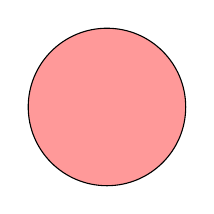
\begin{tikzpicture}
    \begin{scope}[fill opacity = .4]
        
    
       \draw[fill=red](0, 0) circle (1);
       \end{scope}
    \end{tikzpicture}
\end{parag}

\begin{parag}{Le corps des nombre}
    après
\end{parag}

\begin{parag}{Les matrice de taille $2 \times 2$}
    En gros les matrices de taille $2 \times 2$ ne forment pas un corps. Néanmoins il existe des sous-ensebmle de $M_{2\times 2}(\mathbb{R})$ qui sont des corps:
    
\end{parag}
\begin{parag}{Sous-anneaux des matrice de taille $2 \times 2$}
    \begin{enumerate}
        \item Soit $S = \{A \in M_{2\times 2}(\mathbb{R})| A \textbf{ est scalaire}\}$. Alors $S$ fun corps pour la somme et le produit de maitrces. En fait l'application $f: \mathbb{R} \to S$ définie par $f(a) = aI_2$ est un isomorphisme qui identidie $S$ avec le corps des nombres réels.
        \item Soit $M = \{A \in M_{2\times 2}(\mathbb{R})| a_{11} = a_{22} \text{ et } a_{12} = a_{21}\}$. Alors $M$ forme un corps.
    \end{enumerate}
    \\
    On a en premier lieu:
    \[M = \left\{\begin{pmatrix}
        a & b \\ -b & a
    \end{pmatrix}| a, b \in \mathbb{R}\right\}\]
    \begin{enumerate}
        \item A part $\begin{pmatrix}
            0 & 0 \\ 0 & 0
        \end{pmatrix}$, élément neutre pour $t$, toutes les matrices ont un inverse: $\det \begin{pmatrix}
            a & b\\ -b & a
        \end{pmatrix} = a^2 + b^2 \geq 0$ et ce det $= 0$ si et seulement si $a = b = 0$.
        \item Dans $M$ la multiplication est commutative, 
        \[\begin{pmatrix}
            a & b \\ -b & a
        \end{pmatrix}\begin{pmatrix}
            c & d \\ -d & c
        \end{pmatrix} = \begin{pmatrix}
            ac - bd & ad + bc \\ -bc- ad & -bd + ac
        \end{pmatrix} = \begin{pmatrix}
            c & d \\ -d & c
        \end{pmatrix}\begin{pmatrix}
            a & b \\ -b & a
        \end{pmatrix}\]
        \\
        \textbf{Conclusion : } $(M, +, \cdot)$ est un corps. En fait on a un isomorphisme $f : \mathbb{C} \to M$ tel que 
        \[a + bi \to \begin{pmatrix}
            a & b \\ -b & a
        \end{pmatrix}\]
    \end{enumerate}
\end{parag}
\begin{parag}{Arithmétique modulaire}
    Comme pour $\mathbb{F_2} = \{0,1\}$ on peut considérer l'ensemble des nombres entiers $\{0, 1, 2 \dots, n-1\}$.
\end{parag}
\lecture{21}{2024-11-26}{Corps et diagonalisation}{}


\begin{parag}{Arithmétique modulaire}
    Comme pour $\mathbb{F_2} = \{0, 1\}$ on peut considérer l'ensemble des nombres entiers $\{0, 1, 2, \dots, n\}$.
    \\
    On regarde ces nombres comme tous les restes possible de la division par $n$, ce qui nous permet de définir une somme et un produit en calculant dans $\mathbb{Z}$, mais en gardant que le reste de la division. Ainsi:
    \begin{enumerate}
        \item Dans $\{0, 1, 2\}$ on calcule $2 + 2 = 1$
        \item Dans $\{0, 1, 2\}$ on calcule $2^3 =2 $
        \item Dans $\{0, 1, 2, 3, 4\}$ on calcule $3 \cdot 4 = 2$
        \item Dans $\{0, 1, 2, 3, 4\}$ on calcule $1 - 4 = 2 $
        \item Dans $\{0, 1, 2, 3, \dots, 10, 11\}$ on calcule $10 \cdot 6 = 0 $
    \end{enumerate}
\end{parag}

\begin{parag}{Le corps $\mathbb{F_\rho}$}
\begin{subparag}{Proposition}
    \begin{theoreme}{Proposition}
        Lorsque $n$ n'est pas un nombre premier les opérations définies ci-dessus ne forment pas un corps.
    \end{theoreme}
\end{subparag}
\begin{subparag}{Preuve}
    Comme $n$ n'est pas premier, $n = a \cdot b$ pour $1 < a, b < n$.
    Ainsi le nouveau produit $a \cdot b$ est nul. Alors $a$ ne peut pas avoir d'inverse car sinon $b = 1 \cdot b = a^{-1} \cdot 0 = 0$.
\end{subparag}   
\begin{theoreme}
    lorsque $\rho$ est un nombre premier les opérations définies ci-dessus forment un corps $\mathbb{F_\rho}$.
\end{theoreme}
Les seules propriétés qui ne découlent pas de celle de la somme et du produit dans $\mathbb{Z}$ sont l'existence d'opposé et d'inverse.
\begin{subparag}{Preuve}
    \begin{itemize}
        \item Opposé: Si $o \leq k < p$ alors son opposé est $p-k$ car $k + (p-k) = p = 0$.\\
        Si $k = 0$, son opposé est $0$.
        \item Inverse: Soit $0 < k <$, on doit trouver $0 < a  < p$ tel que $a \cdot k = 1$. On considère $\phi : \{0, 1, \dots, p-1\} \to \{0, 1, \dots, p_1\} : x \to x \cdot k $\\
        On montre que $\phi$ est injective, ce qui montrera en même temps que $\phi$ est aussi surjective: il existe un $a$ tel que $\phi(a) = 1$.
    \end{itemize}
    \begin{framedremark}
        C'est le piegeonhole principle en AICC:
        \\
        Si il y a 400 cadeaux avec des noms différents alors chacun a son cadeau si on a 400 éléves, donc si chaque éléments a un $\phi(k)$ qui est différents on a alors chaque cadeau qui est différents, et si on a le même nombre de cadeau et d'éléves alors on a forcémment un cadeau par éléves
    \end{framedremark}
    \begin{itemize}
        \item Pour cela si $0 < x, y<p$, supposons que $\phi(x) = \phi(y)$, on doit montrer que $x = y$. On sait : $x \cdot k = y \cdot k$ ce qui revient à dire $(x-y)\cdot k = 0$,dans $\mathbb{Z} (x-y)\cdot k$ est un multiple de $p$. mais $k$ est un nombre $< p$, donc $p$ divise $x - y$ mais comme à leur tour $0 < x, y < p$, $x = y$
    \end{itemize}
    \begin{framedremark}
        En gros comme $x - y$ est plus petit que $p$ lui même, la seul possibilité pour que se soit vrai, c'est que $x - y = 0$
    \end{framedremark}
\end{subparag}
\begin{subparag}{Exemple}
\begin{enumerate}
    \item Dans $\mathbb{F}_3$, $2^{-1} = 2$
    \item Dans $\mathbb{F}_5, 2^{-1} = 3$ car $2\cdot 3 = 6 = 1$
    \item Dans $\mathbb{F}_p, (p-1)^{-1}  = (-1)^{-1} ) -1 = p-1 $
    \\
    Ou alors $(p-1)(p-1) = p^2-2p + 1 = 1$ car $p^2$ et $-2p$ sont divisibles par $p$.
\end{enumerate}
\begin{framedremark}
    Attention! par exemple
    \[\mathbb{F}_6, \; 2^{-1} \]
    n'existe pas car $6$ n'est pas un nombre premier.
\end{framedremark}
\end{subparag}
\begin{subparag}{Remarque}
\begin{framedremark}
    On va pouvoir former des espaces vectoriels sur $\mathbb{F}_p$ comme:
    \\
    $(\mathbb{F}_p)^n$, $\mathbb{F}_p[t]$ polynôme à coefficient dans $\mathbb{F}_p$ ou alors, $M_{2\times 3}(\mathbb{F}_p)$
\end{framedremark}
\end{subparag}
\end{parag}


\begin{parag}{Critère de diagonalisation}
    En général, pour diagonaliser une matrice sur \R, il faut qu'il y ait assez de valeurs propres réelles \textcolor{red}{et} assez de vecteurs propres.
    \begin{theoreme}
        Une matrice $A$ est diagonalisable sur \R si et seulement si 
        \begin{enumerate}
            \item Le polynôme caractéristique est \textcolor{red}{scindé} sur \R : il se décompose en produit de facteurs $(\lambda - t)$ avec $\lambda \in $ \R
            \item Pour tout $\lambda$, on a $\dim E_\lambda = mult(\lambda)$.
        \end{enumerate}
    \end{theoreme}
    Si $A$ est diagonalisable on forme un base de vecteur propres en réunissant les vecteurs de base de chaque espace propres.
    \begin{subparag}{Exemple}
        Soit $A = \begin{pmatrix}
            -3 & 2 & 2\\
            2 & -3 & 2\\
            2 & 2 & -3
        \end{pmatrix}$. On constate sans faire de calcules:
        \begin{enumerate}
            \item Dans chaque lignes la somme des coefficient vaut $-3 + 2 + 2 = 1$ donc $1$ est valeur propre et $\begin{pmatrix}
                1 \\ 1 \\ 1
            \end{pmatrix}$ est vecteurs propre.
            \item $A + 5I_2 = \begin{pmatrix}
                2 & 2 &2\\
                2 & 2 &2\\
                2 & 2 &2
            \end{pmatrix}$ est de rang $1$ et $\ker (A + 5I_2) = Vect\left\{\begin{pmatrix}
                -1 \\ 1 \\0 
            \end{pmatrix}, \begin{pmatrix}
                -1 \\ 0 \\ 1
            \end{pmatrix}\right\}$ est de $\dim 2$.
            \item Donc $\dim E_1 = 1, \dim E_{-5} = 2$ et on trouve une base de vecteurs propres 
            \[\left(\begin{pmatrix}
                1 \\ 1 \\ 1
            \end{pmatrix}, \begin{pmatrix}
                -1 \\ 1 \\ 0
            \end{pmatrix}, \begin{pmatrix}
                -1 \\ 0 \\ 1
            \end{pmatrix}\right)\]
            \item $c_A(t) = -(t-1)(t+5)^2$
        \end{enumerate}
        Ainsi $ A \approx \begin{pmatrix}
            1 & 0 & 0\\
            0 & -5 & 0\\
            0 & 0 & -5
        \end{pmatrix}$
        \\
        La matrice de changement de base est donc $(Id)_\bmath^{\cmath an} = \begin{pmatrix}
            1 & -1 & -1 \\
            1 & 1 & 0\\
            1 & 0 & 1
        \end{pmatrix} = P$ et $(Id)_{\cmath an}^\bmath = P^{-1}$.
    \end{subparag}
    \begin{subparag}{Suite, changement de base}
        $D = \begin{cases}
            P\cdot A \cdot P^{-1}\\
            P^{-1}\cdot A \cdot P
        \end{cases}$ et $A = P\cdot D \cdot P^{-1}$
    \end{subparag}
\end{parag}

\begin{parag}{Diagonalisabilité : Néthode}
    Soit $T : V \to V$ une application linéaire.
    \begin{enumerate}
        \item Choisir une base $\cmath$ de $V$ (la base canonique si elle existe)
        \item Ecrire la matrice $A = (T)_{\cmath}^\cmath$ de $T$ dans cette base
        \item Calculer le polynôme caractéristique $c_A(t)$.
        \item $c_A(t)$ n'est pas scindé, $A$ n'est pas \textcolor{red}{diagonalisable}.
        \item Si $c_A(t)$ est scindé, extraire les racines de $\lambda$ de $c_A(t)$ et calculer les multiplicité algébrique.
        \item Calculer les espaces propres $E_\lambda$ et les multiplicités géomtrétriques.
        \item Si $\dim E_\lambda = mult(\lambda)$ pour une valeur propre $\lambda$, alors $A$ n'est pas \textcolor{red}{diagonalisable}.
        \item Si $\dim E_\lambda = mult(\lambda)$ pour tout $\lambda$, alors $A$ est \textcolor{green}{diagonalisable}.
    \end{enumerate}
    Dès lors
    \begin{enumerate}
        \item Soit $T : V \to V$ une application linéaire \textcolor{green}{diagonalisable}.
        \item Choisir une base $\bmath_\lambda$ de $E_\lambda$ pour toute valeur propres $\lambda$.
        \item Réunir les $\bmath_\lambda$ pour former une base de $\bmath$ de $V$.
        \item $D = (T)_\bmath^\bmath$ est diagonale. Les valeurs propres apparaissent dans la diagonale dans l'ordre choisi pour construire la base $\bmath$.
        \item Les colonnes de la matrice de changemet de base $P = (Id)_\bmath^\cmath$ sont les vecteurs de $\bmath$ exprimés en cooronnées dans $\cmath$.
        \item $D = P^{-1}AP$ et $A = PDP^{-1}$.
    \end{enumerate}
    \begin{subparag}{Exemple}
        Soit $W$ le plan de $\mathbb{R}^3$ donné par l'équation $x + y + z = 0$. On considère l'application linéaire $T: W \to W$ donnée par la formule :
        \[T\begin{pmatrix}
            -y -z \\ y \\ z
        \end{pmatrix} = \frac{1}{5}\begin{pmatrix}
            9y + z\\
            3y -8z \\
            -12 y + 7z
        \end{pmatrix}\]
        \begin{enumerate}
            \item On vérifie d'abord que $T\vec{w} \in W$ pour tout $\vec{w} \in W$.
            \item On choisit ensuite une base $\cmath$ de $W$, par exemple
            $\left(\begin{pmatrix}
                -1 \\ 1 \\ 0
            \end{pmatrix}, \begin{pmatrix}
                -1 \\0 \\ 1
            \end{pmatrix}\right)$
        \end{enumerate}
        On peut maintenant calculer la matrice $A$ de $T$, par rapport à la base $\cmath$. Il faut toutefois calculer les images des vecteurs de base:
        \begin{align*}
            T(c_1) &= \frac{1}{5}\begin{pmatrix}
                9 \\ 3 \\ -12
            \end{pmatrix} = \frac{3}{5}\begin{pmatrix}
                -1 \\ 1 \\ 0
            \end{pmatrix} - \frac{12}{5}\begin{pmatrix}
                -1 \\ 0 \\ 1
            \end{pmatrix} = \frac{3}{5}c_1 - \frac{12}{5}c_2\\
            T(c_2) &= \frac{1}{5}\begin{pmatrix}
                1 \\ -8 \\ 7
            \end{pmatrix} = -\frac{8}{5}c_1 + \frac{7}{5}c_2
        \end{align*}
        On a donc $A = \frac{1}{5}\begin{pmatrix}
            3 & -8 \\ -12 & 7
        \end{pmatrix}$
        On va donc chercher les valeurs propres:
        \[c_A(t) = \begin{vmatrix}
            \frac{3}{5}-t & -\frac{8}{5}\\
            -\frac{12}{5} & \frac{7}{5} - t
        \end{vmatrix} = t^2 -2t -3 = (t-3)(t+1)\]
        On calcule ensuite les espaces propres:
        \begin{align*}
            E_{-1} &= Vect\left\{\begin{pmatrix}
                1 \\ 1
            \end{pmatrix}\right\}\\
            E_3 &= Vect\left\{\begin{pmatrix}
                -2 \\ 3
            \end{pmatrix}\right\}
        \end{align*}
        ON a donc que la base est donnée par:
        \[\bmath' = \left(\begin{pmatrix}
            1 \\ 1
        \end{pmatrix}, \begin{pmatrix}
            -2 \\ 3
        \end{pmatrix}\right)\]
        Qui est une base de \R$^2$ formé de vecteurs propres de $A$.
        On arrive donc à $A \approx \begin{pmatrix}
            -1 & 0 \\ 0 & 3
        \end{pmatrix} = D$.\\
        On doit revenir à notre problème de départ $T : W \to W$
        \\
        Ces vecteurs sont donnés en coordonnées dans la base $\cmath$ puisque $A$ est la matrice de $T$ par rapport à $\cmath$:
        \[(T)_\cmath^\cmath (x)_\cmath = (T(x))_\cmath\]
        Par exemple $b_1 = c_1 + c_2$. Ainsi
        \[\bmath = \left(\begin{pmatrix}
            -2 \\ 1 \\ 1
        \end{pmatrix}, \begin{pmatrix}
            -1 \\-2 \\ 3
        \end{pmatrix}\right)\]
        La signification géomètrique de $T$ est maintenant transparente.
    \end{subparag}
\end{parag}

\begin{parag}{La trace}
    \begin{defintion}
        Soit $A$ une amtrice $n \times n$. La \textcolor{red}{trace} $Tr A = a_{11} + a_{22} + \cdots + a_{nn}$.
    \end{defintion}
    \begin{subparag}{Exemple}
        Soit $A = \begin{pmatrix}
            a & c \\ b & d
        \end{pmatrix}$. Alors $TrA = a + d$ Or

  \[
c_A(t) = (a - t)(d - t) - bc = t^2 - (a + d)t + (ad - bc) = t^2 - \text{Tr}A \cdot t + \det A
\]
Soit:
\[
A = 
\begin{pmatrix}
a_{11} & a_{12} & a_{13} \\
a_{21} & a_{22} & a_{23} \\
a_{31} & a_{32} & a_{33}
\end{pmatrix}
\quad \text{et} \quad \text{Tr}A = a_{11} + a_{22} + a_{33}.
\]

\[
c_A(t) = (a_{11} - t)(a_{22} - t)(a_{33} - t) + \text{polynôme de degré 1}
= -t^3 + (a_{11} + a_{22} + a_{33})t^2 + \dots
\]
    \end{subparag}
    \begin{subparag}{Proposition}
        \begin{theoreme}
            Soit $A$ une matrice de taille $n \times n$. Alors $(-1)^{n-1}TrA$ est le coefficient de $t^{n-1}$ de $c_A(t)$ et $\det A$ est le coefficient constant
        \end{theoreme}

        \begin{theoreme}{Lemme}
            Soit $A, B, \in M_{n \times n}(\mathbb{R}) $ Alors $Tr(AB) = Tr(BA)$
        \end{theoreme}
        \begin{theoreme}
            Si $A$ est diagonalisable, alors la trace de $A$ est égal à la somme des valeurs propres.
        \end{theoreme}
    \end{subparag}
    \begin{subparag}{Preuve}
        \begin{enumerate}
            \item 
            \begin{align*}
                
            Tr(A\cdot B) &= \sum_{i = 1}^n(A \cdot B)_{ii} = \sum_{i = 1}^n(\sum_{j=1}^n a_{ij}\cdot b_{ji})\\
            &\sum_{j=1}^n(\sum_{i=1}^n b_{ji}\cdot a_{ij})\\
            &= \sum_{j=1}^n (B\cdot A)_{jj} = Tr(BA)
            \end{align*}
            \item Si $A \approx B$, il existe $P$ inversible tel que $A = PBP^{-1}$ et donc 
            \begin{align*}
                Tr(A) = Tr(PBP^{-1}) = Tr(P^{-1}PB) = Tr(B)
            \end{align*}
            Si $A \approx D $ oû $D$ est la diagonale de $A$ alors:
            \[TrA = TrD = \lambda_1 + \cdots + \lambda_n\]
            \textbf{Rappel:} $\det A = \lambda_1\cdot \lambda_2 \cdots \lambda_n$
        \end{enumerate}
    \end{subparag}
    
\end{parag}
\begin{parag}{Deux compléments}
    \begin{theoreme}
        Soit $A$ une matrice carrée telle que $c_A(t)$ est scindé. Alors $A$ est  \textcolor{red}{triangularisable} ($A$ est semblable à une matrice triangulaire).
    \end{theoreme}
    Le théorème suivant affirme que le polynôme caractéristique "\textit{annule}" la matrice $A$.
    \begin{theoreme}{Théorème de Cayley-Hamilton}
        Soit $c_A(t) = t^n + a_{n-1}t^{n-1} + \cdots a_n t + a_0$ le polynôme caractéristique de $A$ alors:
        \begin{formule}
            \[A^n + a_{n-1}A^{n-1} + \cdots + a_1A + a_0I_n = 0\]
        \end{formule}
    \end{theoreme}
    \begin{subparag}{Exemple}
        \[c_B(t) ? t^2 - 5t + 2\]
        Alors $B^2 - 5B + 2I_2 = 0$
    \end{subparag}
\end{parag}

\lecture{22}{2024-11-28}{Orhogonalité}{}

Soit $A$ une matrice diagonalisable. Il existe une matrice inversible $P$ et une matrice diagonale $D$ telles que:
\[A = PDP^{-1}\]
Mais alors on a aussi 
\[A^2 = PDP^{-1}PDP^{-1} = PD^2P^{-1} \text{ et } A^k = PD^kP^{-1}\]


\[
D =
\begin{pmatrix}
\lambda_1 & 0 & \cdots & 0 \\
0 & \lambda_2 & \cdots & 0 \\
\vdots & \vdots & \ddots & \vdots \\
0 & 0 & \cdots & \lambda_n
\end{pmatrix}
\quad \Rightarrow \quad
D^k =
\begin{pmatrix}
\lambda_1^k & 0 & \cdots & 0 \\
0 & \lambda_2^k & \cdots & 0 \\
\vdots & \vdots & \ddots & \vdots \\
0 & 0 & \cdots & \lambda_n^k
\end{pmatrix}
\]

\begin{parag}{Evolution de populations}
    On étudie les populations de Lausanne et du Gros de Vaud. La situation (sans lien avec la réalité du canton) est représenté par la situation suivante:
    \begin{center}
        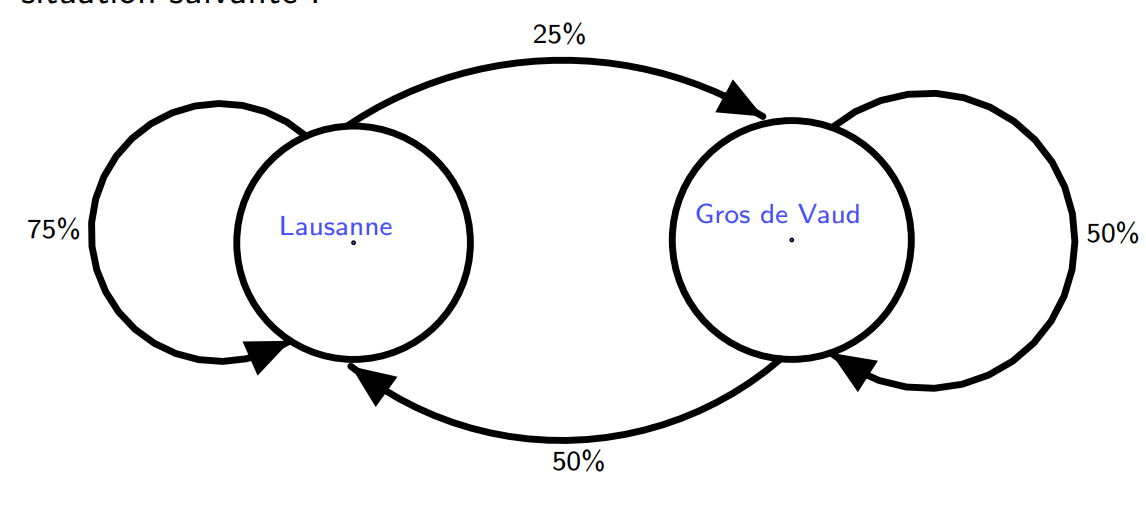
\includegraphics[scale=0.4]{Algèbre linéàaire/Screenshot 2024-11-28 081103.png}
    \end{center}
    Appelons $u_k$ la population urbaine l'année $k$ (en pourcents) et $r_k$ la population rurale.
    \\ 
    On cherche ici à écrire une formule pour décrire tout ça.\\
    \[u_{k+1} = \frac{3}{4}u_k + \frac{1}{2}r_k\]
    
    \[r_{k+1} = \frac{1}{4}u_k + \frac{1}{2}r_k\]
    On a donc:
    \[\begin{cases}
        u_{k+1} = \frac{3}{4}u_k + \frac{1}{2}r_k\\
        r_{k+1} = \frac{1}{4}u_k + \frac{1}{2}r_k
    \end{cases}\]
    Nous avons modélisé matriciellemment cette situtation et posons:
\[A = \begin{pmatrix}
    3/4 & 1/2\\ 1/4 & 1/2
\end{pmatrix}\]
Ainsi:
\[\begin{pmatrix}
    3/4 & 1/2\\ 1/4 & 1/2
\end{pmatrix}\begin{pmatrix}
    u_k \\ r_k
\end{pmatrix} = \begin{pmatrix}
    u_{k+1}\\ r_{k+1}
\end{pmatrix}\]
si bien que:
\[\begin{pmatrix}
    3/4 & 1/2\\ 1/4 & 1/2
\end{pmatrix}^k\begin{pmatrix}
    u_0\\r_0
\end{pmatrix} = \begin{pmatrix}
    u_k \\ r_k
\end{pmatrix}\]
Pour comprendre ce qui se passe dans le futur (lointain), il faut donc calculer $\lim_{k \to \infty} A^k$.
\\
\\
Nous calculons:
\begin{enumerate}
    \item $c_A(t) = (t-1)(t-\frac{1}{4})$
    \item $E_1 = Vect\left\{\begin{pmatrix}
        2 \\ 1
    \end{pmatrix}\right\}$ et $E_{1/4} = Vect\left\{\begin{pmatrix}
        1 \\ -1
    \end{pmatrix}\right\}$
    \item $\bmath = \left(\begin{pmatrix}
        2\\1
    \end{pmatrix}, \begin{pmatrix}
        1 \\ -1
    \end{pmatrix}\right)$ est une base de \R$^2$ formée de vecteurs propres de $A$
    \item $P = (Id)_\bmath^{\cmath an} = \begin{pmatrix}
        2 & 1 \\ 1 & -1
    \end{pmatrix},\; P^{-1} = (Id)_{\cmath an}^\bmath = \frac{1}{3}\begin{pmatrix}
        1 & 1 \\ 1 & -2
    \end{pmatrix}$
    \item On a donc pour la diagonale: $D = \begin{pmatrix}
        1 & 0 \\ 0 & 1/4
    \end{pmatrix}$
    \item \textcolor{red}{Formule de changement de base } : $A^k = PD^kP^{-1}$.
\end{enumerate}
On va donc chercher maintenant à partir de la diagonale avec notre formuel énconcé au point $5$:
\[A^k = \frac{1}{3}\begin{pmatrix}
    2 & 1 \\ 1 & -1
\end{pmatrix}\begin{pmatrix}
    1^k & 0 \\ 0 & \frac{1}{4}^k
\end{pmatrix}\begin{pmatrix}
    1 & 1 \\ 1 & -2
\end{pmatrix} \\
= \frac{1}3{\begin{pmatrix}
    2+\frac{1}{4}^k & 2 -\frac{1}{4}^{k-1}\\
    1 - \frac{1}{4}^k & 1 + \frac{1}{4}^{k-1}
\end{pmatrix}}\]

\begin{align*}
    \begin{pmatrix}
        u_k\\r_k
    \end{pmatrix} = A^k\begin{pmatrix}
        u_0\\r_0
    \end{pmatrix} = \begin{pmatrix}
        1/3(2+\frac{1}{4}^k)u_0 + \frac{1}{3}(2-\frac{1}{4}^{k-1})r_0\\
        1/3(1-\frac{1}{4}^k)u_0 + \frac{1}{3}(1 + \frac{1}{4}^{k-1})r_0
    \end{pmatrix}
\end{align*}
Comme $\lim_{k\to \infty} \frac{1}{4}^k = 0$ on peut facilement trouver que $u_\infty = \frac{1}{3}\cdot2 u_0 = \frac{2}{3}P_0$ où $P_0 = u_0 + r_0$ qui est la population totale
\end{parag}


\chapter{Orthogonalité}
\begin{parag}{non}
    

\begin{enumerate}
    \item \R$^n$ est non seulement un espace vectoriel, c'est un espace \textcolor{red}{euclidien}.
    \item  Nous avons une notion de distance et d'angle
    \item La base canonique est composée de vecteurs \textcolor{red}{orthgonaux} deux à deux et \textcolor{red}{unitaires} (de longueur 1).
\end{enumerate}

\end{parag}

\begin{parag}{Le produit scalaire}
    \begin{definition}
        Soit $\vec{u}, \vec{v}$ deux vecteur de $\mathbb{R}^n$. Le \textcolor{red}{produit scalaire} est
        \begin{formule}
            \[\vec{u}\cdot\vec{v}= \vec{u}^t\vec{v} = u_1v_1 + \cdots + u_nv_n\]
        \end{formule}
    \end{definition}
    \begin{subparag}{Propriétés}
\begin{enumerate}
    \item \textbf{Commutativité} 
    $\vec{u} \cdot \vec{v} = \vec{v} \cdot \vec{u}$
    
    \item \textbf{Distributivité} 
    $\vec{u} \cdot (\vec{v} + \vec{w}) = \vec{u} \cdot \vec{v} + \vec{u} \cdot \vec{w}$
    
    \item \textbf{Compatibilité avec l'action scalaire}
    $\alpha (\vec{u} \cdot \vec{v}) = \vec{u} \cdot (\alpha \vec{v}) = (\alpha \vec{u}) \cdot \vec{v}$
    
    \item \textbf{Positivité} 
    $\vec{u} \cdot \vec{u} \geq 0 \quad \text{et} \quad \vec{u} \cdot \vec{u} = 0 \iff \vec{u} = \vec{0}$
\end{enumerate}

    \end{subparag}
    \begin{subparag}{Preuve}
        Les propriétés $1-3$ sont celles de la multiplication de matrice. Pour $4$, $\vec{u}\cdot\vec{u} = u_1^2 + \cdots + u_n^2\geq 0.$ On a l'égalité si et seulement si tous les $u_1 = 0$.
    \end{subparag}
\end{parag}
\begin{parag}{La norme}
    \begin{definition}
        La \textcolor{red}{longueur} ou \textcolor{red}{norme} d'une vecteur $\vec{u}$ de $\mathbb{R}^n$ est :
        \begin{formule}
            \[||\vec{u}|| = \sqrt{\vec{u}\cdot\vec{u}} = \sqrt{u_1^2 + \cdots + u_n^2}\]
        \end{formule}
    \end{definition}
    Un vecteur de norme $1$ est dit \textcolor{red}{unitaire}. Pour normaliser un vecteur non nul, il suffit de le diviser par sa norme:
    \[
\frac{\vec{u}}{\|\vec{u}\|} =
\begin{pmatrix}
\frac{u_1}{\|\vec{u}\|} \\
\vdots \\
\frac{u_n}{\|\vec{u}\|}
\end{pmatrix}
\quad \text{est unitaire}
\]


\end{parag}
\begin{parag}{La distance}
    \begin{definition}
        La \textcolor{red}{distance} entre deux vecteurs $\vec{u}$ et $\vec{v}$ de \R$^n$ est:
        \begin{formule}
            \[d(\vec{u}, \vec{v}) = ||\vec{u} - \vec{v}||\]
        \end{formule}
    \end{definition}
    \begin{framedremark}
        On voit aussi que cette formule marche dans l'autre sens.\\
        Des vecteurs sont orthogonaux si et seulement si la distance entre $\vec{u}$ et $\vec{v}$ est la même que la distance entre $\vec{u}$ et $-\vec{v}$.
    \end{framedremark}
    \begin{subparag}{Remarque}
        Quelles sont les conséquences de l'égalité $d(\vec
        {u}, \vec{v}) = d(\vec{u}, -\vec{v})$?\\
        Si $||\vec{u} - \vec{v}|| = ||\vec{u} - (-\vec{v})|| = || \vec{u}+\vec{v}||$ alors, $||\vec{u}-\vec{v}||^2 = ||\vec{u} + \vec{v}||^2$ on a le droit de dire ça car une distante est toujours positive.
        \\
        Par la définition de la norme:
        $(\vec{u} - \vec{v})\cdot(\vec{u}-\vec{v}) = (\vec{u}+\vec{v})\cdot(\vec{u}+\vec{v})$.
        \\
        Par la distributivité:
        \[\]
    \end{subparag}
    \begin{definition}
        Deux vecteurs $\vec{u}$ et $\vec{v}$ de $\mathbb{R}^n$ sont \textcolor{red}{orthogonaux} si 
        \begin{formule}
            \[\vec{u}\cdot \vec{v} = 0\]
        \end{formule}
    \end{definition}
        \begin{subparag}{Théorème de pythagore}
            \begin{theoreme}
                Deux vecteurs $\vec{u}$ et $\vec{v}$ sont orthogonaux si et seulement si 
                \[||\vec{u}+\vec{v}||^2 = ||\vec{u}||^2 + ||\vec{v}||^2\]
            \end{theoreme}
        \end{subparag}
        \begin{subparag}{Notation}
            Soit $W$ un sous-espace de $\mathbb{R}^n$. On note $W^\perp$ l'ensemble de tous les vecteurs orthofobaux à $W$. Ainsi;
            \begin{formule}
                \[W^\perp = \{\vec{u} \in \mathbb{R}^n| \vec{u} \cdot \vec{v} = 0 \text{ pour tout } \vec{w} \in W\}\]
            \end{formule}
            C'est un sous-espace de $\mathbb{R}^n$ (série 11)
        \end{subparag}
        \begin{subparag}{Exemple}
            Soit $W$ le sousespace de $\mathbb{R}^3$ donné par 'éaquation $2x -y + 3z = 0$. On veut décrire ce plan et $W^\perp$.
            \\
            On choisit une base de $W$ : 
            \[\bmath = \left(\begin{pmatrix}
                1 \\ 2 \\ 0
            \end{pmatrix}, \begin{pmatrix}
                -3 \\ 0 \\ 2
            \end{pmatrix}\right)\]
            On a donc par sa définition:
            \begin{align*}
              W^\perp &= \{\vec{u} \in \mathbb{R}^3|  \vec
            u\cdot \vec{w} = 0 \;\;\;\forall \vec{w} \in W\}\\  
            &= \{\vec{u} \in \mathbb{R}^3|\vec{u}\cdot(\alpha\vec{b_1} + \beta\vec{b_2}) = 0 \; \forall\alpha, \beta \in \mathbb{R}\}\\
            &= \{\vec{u} \in \mathbb{R}^3| \vec{u}\cdot\vec{b_1} = 0 = \vec{u}\cdot\vec{b_2}\}
            \end{align*}

            
            Si $\vec{u} = \begin{pmatrix}
                a \\ b \\ c
            \end{pmatrix}$ on a alors: 
            $\vec{u} \cdot \vec{b}_1 = a + 2b$ et $\vec{u}\cdot \vec{b_2} = -3a + 2c$
            On cherche donc à résoudre : 
            \[\begin{cases}
                a + 2b = 0\\
                -3a + 2c = 0
            \end{cases}\; \; , W^\perp = Vect\left\{\begin{pmatrix}
                2 \\ -1 \\ 3
            \end{pmatrix}\right\}\]
            \\
            On observe que $\begin{pmatrix}
                2 \\ -1 \\ 3 
            \end{pmatrix}\perp$ le plan d'éq. $2x -y + 3z = 0$
        \end{subparag}

\end{parag}

\begin{parag}{Lien entre perpendicularité et image et noyau}
    \begin{subparag}{Proposition}
        La droite perpendiculaire au plan déquation $ac + by + cz = 0$, et passant par l'origine \R$^3$, est engendrée par $\begin{pmatrix}
            a \\b \\ c
        \end{pmatrix}$.
    \end{subparag}
    \begin{theoreme}
        Soit $A$ une matrice de taille $m \times n$
        \begin{enumerate}
            \item $\ker A = (LignA)^\perp$
            \item $(ImA)^\perp = \ker(A^T)$
        \end{enumerate}
    \end{theoreme}
    \begin{subparag}{Preuve}
        \begin{enumerate}
            \item $A\cdot\vec{c} = \vec{0} \Leftrightarrow \vec{x}\perp$ chaque ligne de $A$.
            \item  $ImA = ColA = Lign(A^T)$ et $[Lign(A^T)]^\perp = \ker(A^T)$
        \end{enumerate}
    \end{subparag}

\end{parag}

\begin{parag}{Calcul d'angle}
 Le produit scalaire permet aussi de calculer l'angle entre deux vecteurs:
 \begin{theoreme}
     Loi du cosinus:
     \[\vec{u}\cdot \vec{v} = ||\vec{u}||\cdot ||\vec{v}||\cos \alpha\]
 \end{theoreme}
 Le produit scalaire de deux vecteurs est:
 \begin{enumerate}
     \item Nul quand $\cos\alpha = 0$ les vecteurs sont perpendiculaire
     \item maximal quand $\cos \alpha = 1$ les vecteurs sont colinéaire et de même sens
     \item minimmal quand $\cos\alpha = -1$.Les vecteurs sont colinéaires et de sens opposé.
 \end{enumerate}
\end{parag}

\begin{parag}{Famille orthogonales}
    \begin{definition}
        Une famille $\{\vec{u_1}, \dots, \vec{u_k}\}$ des vecteurs de $\mathbb{R}^n$ est \textcolor{red}{orthogonale} si $\vec{u_i}\perp \vec{u_j}$ pour tout $i \neq j$. Cette famille est \textcolor{red}{orthonormée} si de plus $||\vec{u_i}|| = 1$ pour tout $i$.
    \end{definition}
    \begin{subparag}{Exemple}
        La base canonique $(\vec{e_1}, \dots, \vec{e_n})$ est orthonormée. En général on appelle Base orthogonale de $W$ une famille orthogonale orfdonnée qui forme une base de $W$. de même pour une base orthonormée.
    \end{subparag}
    \begin{theoreme}
        Une famille orthogonale de vecteurs non nuls est libres.
    \end{theoreme}
    \begin{subparag}{Preuve}
        Soit une famille orthogonale de $\mathbb{R}^n$ avec $\vec{u_i \neq 0 \; \forall 1 \leq i \leq k}$. Soit $\alpha_1, \dots, \alpha_k \in \mathbb{R}$ et supposons $\alpha_1 \vec{u_1} + \cdots + \alpha_k\vec{u_k} = \vec{0}$. \\
        On doit montrer que $\alpha_1 = \cdots = \alpha_k = 0$.
        \\
        On calcule $0 = (\alpha_1\vec{u_1} + \cdots + \alpha_k\vec{u_k})\cdot \vec{u_i}$\\
        Par la ditributivité on a que c'est égal à $ = \alpha_1\vec{u_1}\cdot\vec{u_i} + \cdots + \alpha_k\vec{u_k}\cdot\vec{u_i}$\\
        Mais comme $\vec{u_i}\perp\vec{u_j}$ alors la seule possibilité est que tout les $\alpha_i = 0$
        
        
    \end{subparag}
\end{parag}


\begin{parag}{Coordonnées dans une base orthogonale}
    \begin{theoreme}
        Pour tout vecteur $\vec{w} \in W$, on a $\vec{w} = \alpha_1\vec{u_1} + \cdots + \alpha_k\vec{u_k}$ et 
        \begin{formule}
            \[\alpha_j = \frac{\vec{w}\cdot\vec{u_j}}{||\vec{u_j}||^2}\]
        \end{formule}
    \end{theoreme}
    On voit ici que la preuve sera du même principe que d'autre déjà faite 
    \begin{subparag}{Exemple}
    On construit une base orthogonale de $\mathbb{R}^3$ en commençant avec le plan d'équation $2x - 3y + z = 0$
    On choisit une base:
    \[\bmath = \left(\begin{pmatrix}
        3 \\ 2 \\ 0
    \end{pmatrix}, \begin{pmatrix}
        -2 \\ 3 \\ 13
    \end{pmatrix}\right) \; \text{ qui est une base orthogonale de W}\]
    \[\cmath = \left(\begin{pmatrix}
        3 \\ 2 \\ 0
    \end{pmatrix}, \begin{pmatrix}
        -2 \\ 3 \\ 13
    \end{pmatrix}\right)\]
    \end{subparag}
\end{parag}
\lecture{23}{2024-12-23}{Famille Orthogonales}{}

\begin{parag}{Familles orthogonales}
    \begin{definition}
        Une famille $(\vec{u}_1, \dots, \vec{u}_k)$ de vecteurs $\mathbb{R}^n$ est \textcolor{red}{orthogonale} si $\vec{u}_i \perp \vec{u_j}$ pour tout $i \neq j$. Cette famille est orthonormée si de plus $||\vec{u}_i|| = 1$ pour tout $i$.
    \end{definition}
    \begin{subparag}{Rappel}
        \begin{enumerate}
            \item Deux vecteurs $\vec{u}$ et $\vec{v}$ de $\mathbb{R}^n$ sont \textcolor{red}{orthogonaux} si leur produit scalaire est nul
            \begin{formule}
            \[\vec{u}\cdot \vec{v} = 0\]
            \end{formule}
            \item Par distributivité du produit scalaire, $\vec{u}\perp\vec{a}$ et $\vec{u} \perp \vec{b}$ implique que
            $\vec{u} \perp Vect\{\vec{a}, \vec{b}\}$
        \end{enumerate}
        \begin{theoreme}
            Une famille orthogonale de vecteurs non nuls est libres
        \end{theoreme}
    \end{subparag}
\end{parag}
\begin{parag}{Coordonnées dans une base orthogonale}
    Soit $W$ un sous-espace de $\mathbb{R}^n$ et $(\vec{u}_1, \dots, \vec{u}_k)$ une base \textcolor{red}{orthogonale} de $W$.
    \begin{theoreme}
        Pour tout vecteurs $\vec{w}\in W$, on a $\vec{w} = \alpha_1\vec{u_1} + \cdots + \alpha_k\vec{u_k}$ et
        \[\alpha_j = \frac{\vec{w}\cdot\vec{u_j}}{||\vec{u_j}||^2}\]
    \end{theoreme}
    \begin{subparag}{Exemple}
        On construit une base orthogonale de $\mathbb{R}^3$ en commençant avec le plan d'équation $2x -3y + z = 0$.
        \\
        La méthode de Gausse nous fournit une base, par exemple, quitte à amplifier pour éviter des fractions, $\vec{b_1} = \begin{pmatrix}
            3\\2\\1
        \end{pmatrix} $ et $\vec{b_2} = \begin{pmatrix}
            -1 \\ 0 \\ 2
        \end{pmatrix}$.
        \\
        Or, ces deux vecteurs ne sont pas orthogonaux. Pour trouver un vecteurs de $W$ orthogonal à $\vec{b_1}$, je peux par exemple le choisir de la forme $\begin{pmatrix}
            -2 \\ 3 \\ c
        \end{pmatrix}$, le produit scalaire avec $\vec{b_1}$ vaut bien zéro, mais il faut encore que $c = 13$ pour que l'équation du play $W$ soit satisfaite. Ainsi on obtient une base orthogonale de $W$ avec 
        \[\vec{b_1} = \begin{pmatrix}
            3 \\ 2 \\ 0
        \end{pmatrix}\; \; \vec{b_2} = \begin{pmatrix}
            -2 \\ 3 \\ 13
        \end{pmatrix}\]
        On y ajoute encore $\vec{b_3} = \begin{pmatrix}
            2 \\ -3 \\ 1
        \end{pmatrix} \in W^\perp$ pour avoir une famille orthogonale de $\mathbb{R}^3 $
        \\
        On a donc la famille ordonnée $\bmath = \left(\begin{pmatrix}
            3 \\ 2 \\ 0
        \end{pmatrix}, \begin{pmatrix}
            -2 \\ 3 \\ 13
        \end{pmatrix}, \begin{pmatrix}
            2 \\ -3 \\ 1
        \end{pmatrix}\right)$ est  une famille orthogonale de vecteurs non nuls de $\mathbb{R}^3$, ele en forme donc une base.
        \begin{framedremark}
            Ce qu'on fait ici c'est quon a un plan dans un espace et on y rajouter un vecteurs qui y est orthogonale pour pouvoir avoir accès à tout l'espace, c'est commme si on pouvait "\textit{translater}" le plan dans l'espace.
        \end{framedremark}
        On cherche maintenant $(\vec{u})_\bmath$ qui est donné par:
        \[\vec{u} = \begin{pmatrix}
            1 \\ 1 \\ -1
        \end{pmatrix}\]
        On calcule maintenant $\vec{u}\cdot \vec{b_1} = 5$, $\vec{u}\cdot\vec{b_2} = -12$ et finalement $\vec{u}\cdot \vec{b_3} = -2$.
        \begin{framedremark}
            C'est la même principe qu'en physique lorsqu'un fait des projection du genre $\vec{v}\cdot \hat{e_x}$, on prend la composant sur l'axe du vecteurs.
        \end{framedremark}
        Ensuite afin de pouvoir le récrire dans la base il faut aussi gerer la longueur par rapport au vecteurs $\vec{b_1}\dots$ qui ont leur propre longueur, il font donc faire le ratio ce qui nous force à calculer les normes. $||\vec{b_1}||^2 = 13,\; ||\vec{b_2}||^2 = 182, \; ||\vec{b_3}||^2 = 14$
        \\
        On a qu'utiliser le théorème vu au dessus:
        \[(\vec{u})_\bmath = \begin{pmatrix}
            5/13\\-12/182 \\
            -2/14
        \end{pmatrix} = \begin{pmatrix}
            5/13\\
            -6/91\\
            -1/7
        \end{pmatrix}\]
    \end{subparag}
    \begin{subparag}{schéma du prof}
    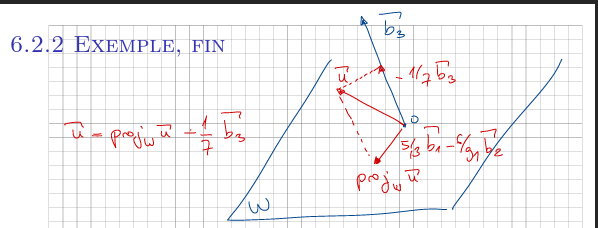
\includegraphics[scale = 0.75]{Algèbre linéàaire/Screenshot 2024-12-04 101913.png}
    
    \end{subparag}
    \begin{framedremark}
        Ce qu'on fait ici c'est prendre le plan $\mathbb{R}^3$ à partir d'une base et donc on prend trois vecteurs pour couvrire tout l'espace. Mais attention à la consigne qui pourrait seulement demander le plan dans une famille de vecteurs orthogonale
    \end{framedremark}
\end{parag}

\begin{parag}{Matrice orthogonales}
    \begin{theoreme}
        Les colonnes d'une matrice $U$ de taille $m\times n$ sont orthonormées si et seulement si $U^TU = I_n$
    \end{theoreme}
    \begin{framedremark}
        ATTENTION, la réciproque ne marche pas $UU^T \neq I_n$ Ca ne marche pas dutout
    \end{framedremark}
    \begin{subparag}{Preuve}
        Si $U = (\vec{u}_1, \dots, \vec{u}_n)$, alors le coefficient $(i, j)$ de la matrice $U^TU$ est exactement $\vec{u_i}^T\vec{u}_j = \vec{u}_i\vec{u}_j$. 
    \end{subparag}
    \begin{definition}
        Une matrice \textcolor{red}{carrée} $U$ est \textcolor{red}{orthogonale} si $U^TU = I_n$. Autremenet dit $U^{-1} = U^T \Leftrightarrow$ colonnes (et lignes!) de $U$ sont orthonormées.
    \end{definition}
    Une matrice orthogonale représente un transofrmation linéaire qui préserve les distantes et l'orthogonalité (c'est donc une \textcolor{red}{isométrie} de $\mathbb{R}^n$, par exemple une rotation ou une symmétrie)
\end{parag}

\begin{parag}{Préservation des longueurs}
    \begin{theoreme}
        Soit $U$ une matrice orthogonale. Alors
        \begin{itemize}
            \item $||U\vec{x}|| = ||\vec{x}||$ pour tout $\vec{x} \in \mathbb{R}^n$
            \item $U\vec{x}\cdot U\vec{y} = \vec{x}\cdot \vec{y}$
            \item $U\vec{x} \perp U\vec{y} \Leftrightarrow \vec{x}\perp \vec{y}$
        \end{itemize}
    \end{theoreme}
    \begin{subparag}{Problème technique}
        J'ai eu un problème avec overleaf donc j'ai pas pu écrire pendant le cours donc j'ai écrir un peu que les théorèmes et moins les exemples
    \end{subparag}
\end{parag}

\begin{parag}{ATTENTION}
    Si $U$ est orthogonale, alors aussi $UU^T = I_n$ Mais
    \begin{itemize}
        \item si $A$ est carrée avec $A^TA$ diagonale, $AA^T$ n'est pas diagonale en général
        \item Si $A$ n'est pas carrée avec $AA^T = I_n$, alors $A^TA \neq I_m$ en général
    \end{itemize}
\end{parag}
\begin{parag}{Projection orthogonale}
    Soit $W$ un sous-espace de $\mathbb{R}^n$ dont on dispose d'une base orthogonale $(\vec{u_1}, \dots, \vec{u}_k)$\\
    Pour $\vec{y} \in \mathbb{R}^n$ on cherche :
    \begin{itemize}
        \item Le vecteurs $\hat{y}\in W$ tel que
        \item le vecteur $\vec{z} = \vec{y}-\hat{y}$ est perpendiculaire à $W$.
    \end{itemize}
    \begin{theoreme}
        Tout vecteurs $\vec{y}$ de $\mathbb{R}^n$ s'écrit de manière unique $\vec{y} = \hat{y}+\vec{z}$ où $\hat{y}\in W$ et $\vec{z}\in W^\perp$
    \end{theoreme}
    \begin{subparag}{Remarque personelle}
        Ce qu'on voit ici c'est qu'il suffit de prendre un vecteurs qui se trouve dans le plan et de le "\textit{monter}" à la hauteur du vecteurs avec $\vec{z}$ qui lui est $\perp W$
    \end{subparag}
\end{parag}

\begin{parag}{Méthode}
    \begin{enumerate}
        \item Vérifier que la base de $W$ est orthogonale! tester toute les pairs $\vec{u_i}\cdot\vec{u}_j = 0$ pour tout les $i \neq j$
        \item Calculer les normes au carré des vecteurs de base $\vec{u_i}$
        \item Calculer les produits scalaires $\vec{y}\cdot\vec{u_i}$
        \item Calculer la projection
        \begin{formule}
            \[\hat{y} = \frac{\vec{y}\cdot \vec{u}_1}{||\vec{u_1}||^2}\vec{u_1} + \cdots + \frac{\vec{y}\cdot\vec{u}_k}{||\vec{u}_k||^2}\vec{u}_k\]
        \end{formule}
        \item Calculer $\vec{z} = \vec{y}-\hat{y}$ et \textcolor{red}{vérifier} que $\vec{z}\perp W$.
        \item \textbf{Remarque} Si $\vec{y} \in W$, alors $\hat{y} = \vec{y}$ et $\vec{z} = \vec{0}$
    \end{enumerate}
\end{parag}
\begin{parag}{Projection, cas d'une base orthonormée}
    Soit $(\vec{u_1}, \dots, \vec{u}_k)$ une base \textcolor{red}{orthonormée} de $W$, alors tous les $\vec{u_i}$ sont unitaires et:
    \begin{align*}
        \text{proj}_w\vec{y} &= (\vec{y}\cdot\vec{u}_1)\vec{u}_1 + \cdots +(\vec{y}\cdot\vec{u}_k)\vec{u}_k\\
        &= (\vec{u}_1^T\vec{y})\vec{u_1} + \cdots + (\vec{u}_k^T\vec{y})\vec{u}_k\\
        &= U\begin{pmatrix}
            \vec{u_1}^T\vec{y}\\
            \vdots\\
            \vec{u}_k^T\vec{y}
        \end{pmatrix} = UU^T\vec{y}
    \end{align*}

    \begin{theoreme}
        Soit $U$ la matrice dont les colonnes sont les vecteurs $\vec{u}_1, \dots, \vec{u}_k$ d'une base \textcolor{red}{orthonormée} de $W$. Alors:

        \begin{formule}
            \[\text{proj}_W\vec{y} = UU^T\vec{y}\]
        \end{formule}
    \end{theoreme}
\end{parag}
\begin{parag}{Approximation quadratique}
    La distance minimale entre un vecteurs $\vec{y}$ et un sous-espace $W$ de $\mathbb{R}^n$ est réalisée par $\vec{z} = \vec{y} - \text{proj}\vec{y}$
    \begin{theoreme}
        Pour tout $\vec{w} \in W$ on a $||\vec{y} - \vec{w}|| \geq ||\vec{y} - \text{proj}_W\vec{y}||$
    \end{theoreme}
    On appelle ce vecteurs $\hat{y}$ la meilleure approcimation quadratique de $\vec{y}$ dans $W$ dans le sens où elle minimuse le carré de la distance qui eest calculée par la somme des carrées des coordonnées.
    \begin{subparag}{Idée de la preuve}
            L'idée est d'écrire un vecteurs $\vec{w}$ de $W$ de manière compliquée $\vec{w} = \hat{y} + (\vec{w} - \hat{y})$ afin de diviser en deux parti le vecteurs une qui est dans $W^\perp$ et l'autre dans $W$.
    \end{subparag}
\end{parag}

\begin{parag}{Le procédé de Gram Schmidt}
    \begin{itemize}
        \item \textbf{But} Trouver une base orthogonale ou rthonormée d'un sous-espace $W$ de $\mathbb{R}^n$
        \item \textbf{Idée} Utiliser de manière inductive les projections orthogonales. On considère dans $\mathbb{R}^4$ l'hyperplan $W$ donnée par l'équation
        \[x_1 + 2x_2 + x_3 + x_4 = 0\]
    \end{itemize}
    \begin{enumerate}
        \item On cherche d'abord une base, par exemple celle faite avec la méthode de gausse:
        \[\bmath = \left(\begin{pmatrix}
            -2 \\ 1 \\ 0 \\ 0
        \end{pmatrix}, \begin{pmatrix}
            -1 \\ 0  \\ 1 \\ 0
        \end{pmatrix}, \begin{pmatrix}
            -1 \\ 0 \\ 0 \\ 1
        \end{pmatrix}\right)\]
        on note les vecteurs $\vec{b_1}, \vec{b_2}, \vec{b_3}$
        \item On garde le premier vecteurs intacte et on va construire les autres vecteurs en fonction de celui la et donc
        \[\vec{c_1} = \vec{b_1}\]
        On projette $\vec{b_2}$ sur $Vect\{\vec{c_1}\}$ et on choisira $\vec{c_2} = \vec{b_2} - \hat{b_2}$.
        \item proj$_{Vect\{\vec{b_1}\}}\hat{b}_2 = \frac{\vec{b_1}\cdot\vec{b_2}}{||\vec{b_1}||^2}\vec{b_1} = \frac{2}{5}\vec{b_1} = \begin{pmatrix}
            -4/5\\2/5\\ 0\\0 
        \end{pmatrix}$
        \\
        On change $\vec{b_2}$ pour le rendre orthogonal à $\vec{c_1}$ :\\
        Et donc $\vec{c_2} = \vec{b_2}-\hat{b_2} = \begin{pmatrix}
            -1/5\\ -2/5 \\ 1 \\ 0
        \end{pmatrix}$
        \end{enumerate}
        Maintenant que nous avons une base orthogonale du plan $V = Vect\{\vec{b_1}, \vec{b_2}\}$, à savoir $(\vec{c_1}, \vec{c_2}$, les formules de projection sont à notre disposition pour calculer $\hat{b}_3 = \text{proj}_V\vec{b}_3$ et $\vec{c_3} = \vec{b_3} - \hat{b}_3$, où $\vec{b_3} = \begin{pmatrix}
            -1 \\ 0 \\ 0 \\ 1
        \end{pmatrix}$
        \\
        On cherche maintenant $\hat{b}_3 = \frac{\vec{b}_3 \cdot \vec{c}_1}{||\vec{c}_1||^2}\vec{c_1} + \frac{\vec{b}_3 \cdot \vec{c_2}}{||\vec{c_2}||^2}\cdot\vec{c_2} = \cdots = \begin{pmatrix}
            -5/6 \\ 1/3 \\ 1/6 \\0
        \end{pmatrix}$
        \\ Et donc:
        \[\vec{c_3} = \vec{b_3} - \hat{b}_3 = \begin{pmatrix}
            -1/6 \\ -1/3 \\ -1/6 \\ 1
        \end{pmatrix}\]
        Nous avons ainsi contrsuire une base orthogonale $\cmath = (\vec{c_1}, \vec{c_2}, \vec{c}_3)$ de $W$. elle a les propriétés suivantes:
        \begin{itemize}
            \item Le vecteur $\vec{c_1} = \vec{b_1}$
            \item Le vecteurs $\vec{c_k}$ est combinaison linéaire des vecteurs $\vec{b_1}, \dots, \vec{b_k}$, en particulier c'est un vecteurs de $W$.
        \end{itemize}
\end{parag}

\lecture{24}{2024-12-05}{moindre carré équation normale et les corps}{}


\begin{parag}{Suite de l'exemple}
    
\end{parag}
\begin{parag}{Rappels}
    Soit $A$ une matrice de taille 
    $n \times m$. Alors $A^T$ est de taille $m \times n$.
    \begin{enumerate}
        \item Les lignes de $A^T$ sont les \textcolor{red}{colonnes} $\vec{a_i}$ de $A$
        \item $A^T\vec{x} = \vec{0}$ si et seulement si $\vec{x} \perp ImA$
        \item Les coefficients $(A^TA)_{ij}$ sont les produits scalaires $\vec{a_i} \cdot \vec{a}_j$
        \item Les colonnes de $A$ sont orthogonales si et seulement si $A^TA$ est diagonale
        \item Les coefficients de $AA^T$ sont les produits scalaires des \textcolor{red}{lignes} de $A$
        \item Les lignes de $A$ sont orthogonales si et seulement si $AA^T$ est diagonale
    \end{enumerate}
\end{parag}

\begin{parag}{Le procédé de Gram-Schmidt : Théorie}
    \textbf{But} trouver une base orthogonale ou orthonromée d'un sous-espace $W$ de $\mathbb{R}^n$.
    \\
    \textbf{Idée} utilise de manière inductive les projection orthogonales.
    \begin{theoreme}
        Soit $(\vec{u_1}, \dots, \vec{u_k})$ une base de $W$, sous-espace de $\mathbb{R}^n$\\
        Les vecteurs suivant forment une base orthogonale de $W$
        \begin{enumerate}
            \item $\vec{v_1} = \vec{u_1}$
            \item $\vec{v_1} = \vec{u_2} - \frac{\vec{u_2}\cdot \vec{v_1}}{||\vec{v_1}||^2}\vec{v_1}$
            \item $\vec{v_k} = \vec{u_k} - \frac{\vec{u_k}\cdot\vec{v_1}}{||\vec{v_1}||^2}\vec{v_1} - \cdots - \frac{\vec{u}_k\cdot\vec{u}_{k-1}}{||\vec{v}_{k-1}||^2}\vec{v}_{k-1}$
        \end{enumerate}
    \end{theoreme}
\end{parag}

\begin{parag}{Factorisation $QR$}
    \begin{definition}
        Soit $A$ une matrice $m \times n$ dont les colonnes sont libres. Alors il existe une factorisation $A = QR$ où les colonnes de $Q \in M_{m\times n}(\mathbb{R})$ sont \textcolor{red}{orthonormées} et $R\in M_{n\times n}(\mathbb{R})$ est triangulaire supérieure et inversible avec des coefficients diagonaux strictement positifs.
    \end{definition}
    \begin{subparag}{Preuve}
        L'idée de la preuve et d'applique la méthode de Gram-Schmidt pour obtenir une base orthogonale $Q$ de $ImA$ à partir des colonnes de $A$ (sans en changer l'ordre), puis on normlaise les vecteurs. On forme $Q$ avec ces vecteurs (colonnes).
        \\
        La $k$-ème colonne de $A$ est combinaison linéaire des $k$ première colonnes de $Q$ et le dernier coefficients est toujours positif. On constate cela en utilisant les formules de Gram-Schmidtage, ou alternativement on se souvient que la base orthogonale construire consiste é soustraire à $\vec{a}_k$ sa projection orthogonale sur l'espace engendrés par les colonnes précédentes. Après normalisation le k-ème coefficient reste positif.
        \\
        La matrice $R$  a pour colonnes ces coefficient $\vec{r}_k = (\vec{a}_k)_Q$
    \end{subparag}

    \begin{subparag}{Exemple}
        Soit $A = \begin{pmatrix}
            1 & 0\\ 1 & 1\\
            1 & 1 \\
             0 & 1
        \end{pmatrix}$. On cherche sa factorisation $QR$.
        \\
        \begin{enumerate}
            \item $\vec{c_1} = \begin{pmatrix}
                1  \\ 1 \\ 1 \\ 0
            \end{pmatrix}$, $\vec{c_2} = \vec{a_2} - \hat{a}_2$\\
            \[\hat{a}_2 = \frac{\vec{a}_2\cdot\vec{c_1}}{||\vec{c_1}||^2}\cdot \vec{c_1} = \frac{2}{3}\begin{pmatrix}
                1 \\ 1 \\ 1 \\ 0
            \end{pmatrix} \; \; \; \vec{c_2} = \begin{pmatrix}
                -2 \\ 1 \\ 1 \\ 3
            \end{pmatrix}\]
            \item Normalisation: $\vec{q_1} = \begin{pmatrix}
                1/\sqrt{3}\\
                1/\sqrt{3}\\
                1/\sqrt{3}
                \\
                0
            \end{pmatrix}$, ensuite $\vec{q_2} = \frac{\vec{c_2}}{||\vec{c_2}||} = \frac{\vec{c_2}'}{||\vec{c_2}||'}$
            \[= \begin{pmatrix}
                -2/\sqrt{15}\\
                1/\sqrt{15}\\
                1/\sqrt{15}\\
                3/\sqrt{15}
            \end{pmatrix}\]
        \item \[Q = \begin{pmatrix}
            1/\sqrt{3} & -2/\sqrt{15}\\
            1/\sqrt{3} & 1/\sqrt{15}\\
            1/\sqrt{3} & 1/\sqrt{15}\\
            0 &3/\sqrt{15}
        \end{pmatrix}\]   
        \item écrire $\vec{a_1}, \vec{a_2}$ comme combiaison linéaire de $\vec{q_1}, \vec{q_2}$.
        \begin{itemize}
            \item $\vec{a_1} = \vec{c_1} = \sqrt{3}\vec{q_1}$, par la suite 
            $\vec{a_2} = \vec{c_2} + \hat{a}_2 = \frac{\sqrt{15}}{3}\begin{pmatrix}
                -2 \\ 1 \\ 1 \\ 3
            \end{pmatrix} + \frac{2}{3}\begin{pmatrix}
                1 \\ 1 \\ 1 \\ 0
            \end{pmatrix}$
            \item $\vec{c_2} = \frac{\sqrt{15}}{3}\cdot\begin{pmatrix}
                -2/\sqrt{15} \\ 1/\sqrt{15} \\ 1/\sqrt{15} \\ 3/\sqrt{15}
            \end{pmatrix} =  \frac{\sqrt{15}}{3}\vec{q_2} + \frac{2\sqrt{3}}{3}\vec{q_1}$
        \end{itemize}
        On a donc 
        \[ R = \begin{pmatrix}
            \sqrt{3} & \frac{2\sqrt{3}}{3}\\
            0 & \frac{\sqrt{15}}{3}
        \end{pmatrix}\]
        $R$ est la matrice qui a dans ses coefficients de $\vec{a_1}$ et dans sa deuxième colonnes les coefficients de $\vec{a_2}$
        \end{enumerate}
        C'est une méthode qui peut s'utiliser dans la pratique, on l'utilise dans la méthode des moindre carées
    \end{subparag}
\end{parag}

\begin{parag}{Méthode des moindre carrés}
    On chercher la "\textit{meilleure solution possible}" d'un système \textcolor{red}{incompatible} $A\vec{x} = \vec{b}$, où $A$ est une matrice $m \times n$.
    \begin{definition}
        Un vecteurs $\hat{x} \in \mathbb{R}^n$ est une \textcolor{red}{solution au sens des moindres carrés} pour le système $A\vec{x} = \vec{b}$ si, pour tout $\vec{x} \in \mathbb{R}^n$
        \begin{formule}
            \[||\vec{b}-A\hat{x}|| \leq ||\vec{b} - A\vec{x}||\]
        \end{formule}
        
    \end{definition}
    Comme $A\vec{x} \in ImA$, le système est incompatible si $\vec{b} \notin ImA$. Le vecteur le plus proche de $\vec{b}$ dans $ImA$ est sa projection orthogonale
    \begin{formule}
        \[\hat{b} = \text{proj}_{ImA}\vec{b}\]
    \end{formule}
    \begin{subparag}{Problème équivalent}
        pour trouver les solutions \hat{x} du système incompatible
        \[A\vec{x} = \vec{b}\]
        Au sens des moindre carrés, il faut résoudre le système
        \begin{formule}
            \[A\hat{x} = \hat{b}\]
        \end{formule}
        \begin{framedremark}
            Il y a en général une infinité de solution au sens des moindres carrés, à moins que l'application linéaire représentée par $A$ ne soit injective.
        \end{framedremark}
        Supposons que $\hat{x}$ soit solution au sens des moindres carrésm si bien que $A\hat{x} = \hat{b} = $ proj$_{ImA}\vec{b}$
        \\
        Alors $\vec{b} - \hat{b} \perp ImA$ et $\vec{b} - \hat{b} = \vec{b} - A\hat{x}$ donc $\vec{b} - A\hat{x} \perp \vec{a_i} \; \; \; \forall i$ Autrement dit:
        \[\vec{a_i}(\vec{b} - A\hat{x}) = 0 \; \; \forall i\]
        Et que donc on peur le réécrire
        \[\vec{a_i}^T(\vec{b} - A\hat{x}) = \vec{a_i}^T\vec{b} - \vec{a}_i^TA\hat{x}\]
        Ainsi
        \begin{equation}
            A^T\cdot\vec{b} = A^TA\hat{x}
        \end{equation}
        $\hat{x}$ est solution de l'équation  (1) 
        
    \end{subparag}
\end{parag}
\begin{parag}{Equation normale}
\begin{theoreme}
    

l'ensemble des solutions $A\vec{x} = \vec{b}$ au sens des moindres carrés est égal à l'ensemble non-vide des solutions de l'\textcolor{red}{équation normale}:
\begin{formule}
    \[A^TA\hat{x} = A^T\vec{b}\]
\end{formule}
\end{theoreme}
\begin{subparag}{Preuve}
    Soit $\hat{x}$ une solution de l'équation normale. Nous devons montrer que $A\hat{x} = \hat{b}$. Nous savons que $A^T(\vec{b} - A\hat{x}) = \vec{0}$. Le vecteurs $\vec{z} = \vec{b} - A\hat{x}$ est donc orthogonal à $ImA$. Mais alors 
    \begin{formule}
        \[\vec{b}  = A\hat{x} + \vec{z}\]
    \end{formule}
    Avec $A\hat{x}\in ImA$ et $Z \in (ImA)^\perp$. Cette écriture est \textcolor{red}{unique} ainsi;
    \[A\hat{x} = \hat{b}\]
\end{subparag}
\end{parag}
\begin{parag}{Question de l'unicité}
    Soit $\hat{x}$ une solution au sens des moindres carrées du systèmes $A\vec{x} = \vec{b}$
    \begin{definition}
        La norme du vecteurs $\vec{b}-A\hat{x}$ est appelée \textcolor{red}{àcart quadratique}
    \end{definition}
    \begin{theoreme}
        La solution $\hat{x}$ au sens des moindres carrées est unique si et seulement si les colonnes de $A$ sont libres, ce qui est équivalent à exiger que la matrice $A^TA$ est inversible
    \end{theoreme}
    Si $A^TA$ est inversible, alors on tire de $
    A^TA\hat{x} = T\vec{b}$ que 
    \begin{formule}
        \[\hat{x} = (A^TA)^{-1}A^T\vec{b}\]
    \end{formule}
    \begin{subparag}{Preuve}
        Supposons d'abord que les colonnes de $A$ sont libres, si bien que le noyau de $A$ est nul. On va montrer que la matrice carrée $A^TA$ est inversible en prouvant que son noyau est nul.
        \\
        Supposons que $A^TA\vec{x} = \vec{0}$, alors $A\vec{x} \perp ImA$ or $A\vec{x} \in ImA$ et aussi $(ImA)^\perp$. Donc $A\vec{x} = \vec{0}$. Comme $\ker A = \{\vec{0}\}, \; \vec{x} = \vec{0}$.
        \\
        Réciproquement, si $A^TA$ est inversible, $A^TA$ est injective. Pour montrer que les colonnes de $A$ sont libres calculons le noyau de $A$. Si $A\vec{x} = \vec{0}$, Alors $A^TA = \vec{x} = A^T\vec{0} = \vec{0}$. Par hypothèse $\vec{x} = \vec{0}$
    \end{subparag}
\end{parag}
\begin{parag}{Le corps $\mathbb{F}_4$}
    Nous avons rencontré les corps $ \mathbb{F}_p$ qui ont un nombre $p$,premier, d'éléments. Il s'agit des nombres entiers \textcolor{red}{modulo $p$} que l'on considère comme le restes possibles de la division par $p$.
    \begin{framedremark}
        Les entiers modulo $4$ ne forment pas un corps car $2 \cdot 2 = 0$. Le produit $\mathbb{F}_2 \times \mathbb{F}_2$ non plus car $(1, 0) \cdot (0, 1) = (0, 0)$.
    \end{framedremark}
    Nous allons maintenant remplacer les entiers par les polynômes $\mathbb{F}_2[t]$ et la division euclidienne par la division polynomiale.
    \begin{enumerate}
        \item les restes de la division par un polynôme de degré plus petit, on travaille donc dans l'ensemble
        \[\{0, 1, t, t+1\}\]
        Nous connaissons tous les polynômes de degré $2$, il s'agit de $t^2 = t\cdot t, t^2 + t = t(t+1), t^2+1 = (t+1)^2$ et $t^2 + t + 1$
    \end{enumerate}
    \begin{framedremark}
        Si on choisit un polynôme non irréductible, le résultats peut être divisé et donc le produit est nul.
    \end{framedremark}
    \begin{subparag}{L'addition dans $
    \mathbb{F}_4$}
    Le produit est donéée par le produit des polynôme. Nous avions calculé le produit $t\cdot t$ par division euclidienne, on peut aussi simplement utiliser le fait que $t^2 + t + 1 = 0$ dans $\mathbb{F}_4$
    \[t\cdot t = t^2 = t^2 + t + 1 + t + 1 = t + 1 \text{ et } t(t+1) = t^2 + t + 1 + 1 = 1\]
        
       
           \begin{tabular}{|c||c|c|c|c|}
           \hline
               $\cdot$ &0  & 1 & $t$ & $t+1$\\
               \hline
               \hline
               $0$ & 0 & 1 & t & $t+1$\\
               \hline
                1&0& 1 & $t$ & $t+1$ \\
                \hline
                $t$& 0 & $t$ & $t+1$ &1 \\
                \hline
                $t+1$& 0 & $t+1$ & $1$ & $t$\\
                \hline
           \end{tabular}
        \\
        Les autres produits manquants s'effectuent de la même manière.
        
    \end{subparag}
\end{parag}
\lecture{25}{2024-10-12}{corps $\mathbb{F}_4$}{}

\begin{parag}{La multiplication dans $\mathbb{F}_4$}
    
        Pour ne pas confondre l'indéterminée $t$ des polynômes et l'élément $t$ donné comme reste de division, on choisit d'appeler $\alpha$ le reste $t$ ou plus précisément la classe $[t]$ de $t$ dans "\textit{l'anneau des polynôme $\mathbb{F}_2[t]$ modulo $t^2 + t + 1$}"
        \begin{enumerate}
            \item Comme \textcolor{red}{ensemble} $\mathbb{F}_4 = \{0, 1, \alpha, \alpha + 1\}$
            \item \textcolor{red}{l'addition} est celle des polynômes, chaque éléments est son propres opposé.
            \item la \textcolor{red}{multiplication} est celle des polyôme, modulo $t^2 + t + 1$, en particulier $\alpha^2 = \alpha + 1$. On a donc aussi $\mathbb{F}_4 = \{0, 1, \alpha, \alpha^2\}$   
        \end{enumerate}
        \begin{framedremark}
            Ici on a choisi $t^2 + t + 1$ pour pouvoir construire nos calcul, mais le critère pour choisir est que c'est un polynôme dans $\mathbb{F}_2$ avec des coefficient irréductible
        \end{framedremark}
        \begin{subparag}{Le polynôme $t^2 + t + 1 \in \mathbb{F}_4[t]$}
            Le polynôme $p(t) = t^2 + t + 1 \in \mathbb{F}_2[t]$ est irréductible, mais on peut aussi le voir comme un polynôme de $\mathbb{F}_4[t]$, car ses coefficients sont dans $\mathbb{F}_2 \subset \mathbb{F}_4$.
            \\
            Calculons $p(\alpha)$
            \[p(\alpha) = \alpha^2 + \alpha + 1 = \begin{cases}
                \alpha + 1  + \alpha + 1 = 2\alpha + 2  = 0\\
                [t]^2 + [t] + 1  = [t^2 + t + 1] = 0
            \end{cases}\]
            le deuxième cas est juste par la définition de $+$ et $\cdot $ dans $\mathbb{F}_4$\\
            Donc, $t-\alpha = t + \alpha$ divise $t^2 + t + 1$ dans $\mathbb{F}_4$. Effectuons la divisions eucidienne. On obtient $t^2 + t + 1 = (t+\alpha)(t + \alpha + 1)$
        \end{subparag}
        \end{parag}

        \begin{parag}{Régression linéaire : Objectif}
            On se donne un "\textit{nuage}" de points dans le plan, donnés par leurs ordonnées ($x_1, y_1), \dots, (x_n, y_n)$ et on aimerait trouver la droite qui donne la meileures approximation :
            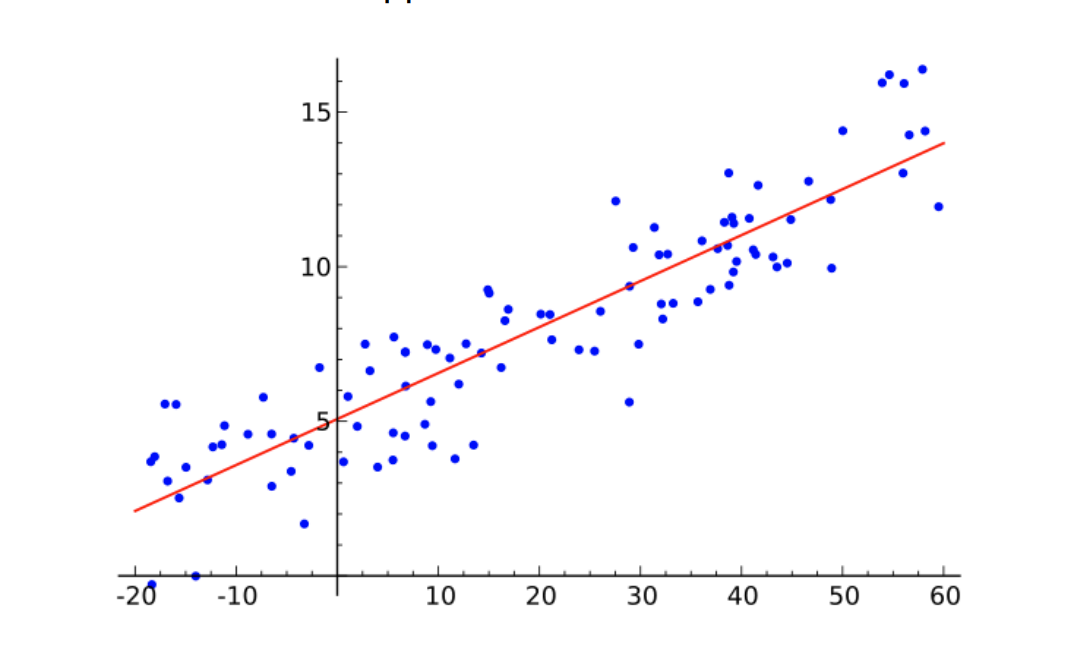
\includegraphics[scale=0.3]{Algèbre linéàaire/Screenshot 2024-12-10 153727.png}
            On cherche la droite d'équation $y = at + b$ la plus proche des points $(x_1, y_1)\dots (x_n, y_n)$ dans le sens où les distances verticales entre les point et la droite sont minimisées (voici un exemple tié de UC Buisness Analytics R programming Guide)
            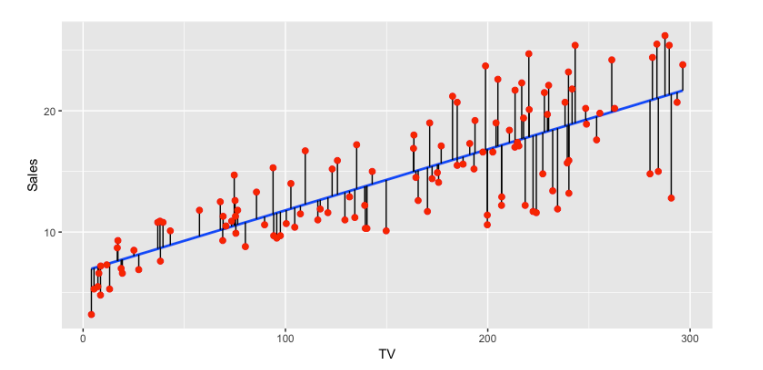
\includegraphics[scale = 0.5]{Algèbre linéàaire/Screenshot 2024-12-10 153930.png}
        \end{parag}
        \begin{parag}{Forme Matricielle}
            On écrit le système ci-dessus sous forme matricielle 
            \[\begin{pmatrix}
                x_1  & 1 \\ \vdots & \vdots \\ x_n & 1
            \end{pmatrix}\begin{pmatrix}
                a \\ b
            \end{pmatrix} = \begin{pmatrix}
                y_1 \\ \vdots \\ y_n
            \end{pmatrix}\]
            et on utilise l'équation normale pour résoudre :
            \[\begin{pmatrix}
                \sum (x_i^2 & \sum x_i\\
                \sum x_i & n
            \end{pmatrix}\begin{pmatrix}
                \hat{a}\\ \hat{b}
            \end{pmatrix} ) \begin{pmatrix}
                \sum x_iy_i \\ \sum y_i
            \end{pmatrix}\]
            \begin{subparag}{exemple}
                On cherche la droite de régression linéaire pour les points $(-2, -1), (0, 1), (2, -2), (4, 1)$
                \[A  = \begin{pmatrix}
                    -2 & 1 \\ 0 & 1 \\ 2 & 1 \\ 4 & 1
                \end{pmatrix} \; \; \; \vec{b} = \begin{pmatrix}
                    -1 \\ 1 \\-2\\ 1
                \end{pmatrix} \; \; \; \; A^T A= \begin{pmatrix}
                    24 & 4 \\ 4 & 4
                \end{pmatrix}\]
                \begin{align*}
                    A^T \vec{b} = \begin{pmatrix}
                        2 \\ -1
                    \end{pmatrix}
                \end{align*}
                On doit résoudre le système $A^TA \cdot \hat{a} = \hat{b} $
                Ce qui nous donne
                $\left(
                \begin{array}{cc|c}
                    24 &4 & 2  \\
                     4&4 & -1 
                \end{array}\right) \to \left(
                \begin{array}{cc|c}
                    1 &0 & 3/20  \\
                     0&1 & -2/5 
                \end{array}\right) $ et donc, $y = \frac{3}{20}t - \frac{2}{5}$
            \end{subparag}
            \begin{framedremark}
                la droite qu'on trouve est toujours unique, a part dans le cas ou le noyau de la matrice n'est pas null, et le seul moyen d'y arriver et que la matrice soit $\begin{pmatrix}
                    1 &1 \\
                    \vdots  & \vdots\\
                    1 & 1
                \end{pmatrix}$ ce qui ferait que tout les points se trouvent au même endroits.
            \end{framedremark}
        \end{parag}
        \begin{parag}{Debriefing sur le produit scalaire}
            Nous avons utilisé jusqu'ici le produit scalaire standard dans $\mathbb{R}^n$. Les propriétés du produit scalaire font que d'associer à une paire de vecteurs $\vec{u}$ et $\vec{v}$ le produit $\vec{u}\cdot \vec{v}$ est une opération linéaire en chaque variable.
            \begin{enumerate}
                \item $\vec{u}\cdot(\vec{v}+\vec{w}) = \vec{u}\cdot\vec{v} + \vec{u}\cdot\vec{w}$
                \item $\vec{u}\cdot(\alpha\vec{v}) = \alpha(\vec{u}\cdot \vec{v})$
                \item $(\vec{u}+\vec{v}) \cdot \vec{w} = \vec{u}\cdot\vec{w} + \vec{v}\cdot \vec{w}$
                \item $(\alpha\vec{u})\cdot \vec{v} = \alpha(\vec{u}\cdot\vec{v})$
            \end{enumerate}
        \end{parag}
        \begin{parag}{Formes bilinéaires}
            Ceci nous motive à introduire un nom à d'autre application de deux variable, définies en général sur un espace vectoriel arbitraire.
            \begin{deinition}
                Soit $V$ un espace vectoriel. Une \textcolor{red}{forme bilinéaire symétrique} est une application $V \times V \to \mathbb{R}$ qui associe à tout couple de vecteurs $(u, v)$ un nombre réel $\langle u, v \rangle$ tel que
                \begin{enumerate}
                    \item commutativité $\langle u, v \rangle ) \langle v, u \rangle$
                    \item distributivité $\langle u + u', v \rangle = \langle u, v \rangle + \langle u' , v \rangle$
                    \item linéairité $\langle \alpha u, v \rangle = \alpha \langle u, v \rangle$
                \end{enumerate}
                \begin{framedremark}
                    Une forme linéaire est une application linéaire $V \to \mathbb{R}$
                \end{framedremark}
            \end{deinition}
            \begin{subparag}{Exemple}
                Le produit scalaire standard de $\mathbb{R}^2$ est une forme bilinéaire symétrique.
                \\
                Il y a de nombreuse autres formes bilinéaires symétriques. Par exemple $\langle \begin{pmatrix}
                    u_1 \\ u_2,  
                \end{pmatrix}, \begin{pmatrix}
                    v_1 \\ v_2
                \end{pmatrix}\rangle = 7u_1v_1 + 2u_1v_2 + 2u_2v_1 + 4u_2v_2$
            \end{subparag}
        
        \end{parag}

        \begin{parag}{Matrices symétriques}
            \begin{subparag}{Proposition}
                \begin{theoreme}
                    On représente une forme bilinéaire symétrique sur $\mathbb{R}^n$ par une matrice symétrique $A$ carrée de taille $n \times n$.
                \end{theoreme}
            \end{subparag}
            \begin{subparag}{Preuve}
                On pose $a_{ij} = \langle e_i, e_j\rangle = \langle e_j, e_i \rangle = a_{ji}$ si bien que 
                \begin{formule}
                    \[\langle u, v \rangle  = u^TAv\]
                \end{formule}
                En effet, $u = u_1e_1 + \cdots +u_ne_n$ et $v = v_1e_1 + \cdots + v_ne_n$. Alors:
                \[\langle e, v \rangle )\sum_i \sum_j u_iv_j\langle e_i, e_j\rangle = \sum_i \sum_j u_iv_ja_{ij} = \sum_i u_i\left(\sum_j a_{ij}v_j \right)\]
                \[= \sum_i u_i(Av)_i = u^TAv\]
            \end{subparag}
            \begin{subparag}{Exemple}
                Le produit scalaire standard de $\mathbb{R}^2$ est une forme bilinéaire symétrique représentée par la matrice $I_2$
                \\
                En effet $\langle \vec{e_i}, \vec{e_j} \rangle = \delta_{ij} \begin{cases}
                    0 \text{ si } i \neq j\\
                    1 \text{ si } i =j
                \end{cases}$
                La forme bilinéaire symétrique
            \[\langle \begin{pmatrix}
                u_i \\ u_2
            \end{pmatrix}, \begin{pmatrix}
                v_1 \\ v_2
            \end{pmatrix}\rangle = 7u_1v_1 + 2u_1v_2 + 2u_2v_1 + 4u_2v_2\]
            $\langle \vec{e_1}, \vec{e_1}\rangle =\langle \begin{pmatrix}
                1 \\ 0
            \end{pmatrix}, \begin{pmatrix}
                1 \\ 0
            \end{pmatrix} \rangle = 7 \dots A = \begin{pmatrix}
                7 & 2 \\ 2 & 4
            \end{pmatrix}$
            \\
            \[\langle \begin{pmatrix}
                u_1 \\ u_2
            \end{pmatrix}, \begin{pmatrix}
                v_1 \\ v_2
            \end{pmatrix}\rangle = (u_1, u_2)\begin{pmatrix}
                7 & 2\\ 2 & 4
            \end{pmatrix}\begin{pmatrix}
                v_1 \\ v_2
            \end{pmatrix}\]
            \end{subparag}
        \end{parag}
        \begin{parag}{Espace préhilbertiens}
            Le produit scalaire euclidien défini aussi une norme :
            \[\vec{u}\cdot \vec{u} = ||\vec{u}||^2 \geq 0\]
            On arrive ici à la notion de produit scalaire dans le sens large.
            \begin{definition}
                Soit $V$ un espace vectoriel. Un \textcolor{red}{produit scalaire} est une forme bilinéaire symétrique $V \times V \to \mathbb{R}$ telle que 
                \begin{enumerate}
                    \item commutativité $\langle u, v \rangle = \langle v, u\rangle$ pour tous $u, v \in V$
                    \item distributivité $\langle u + u', v\rangle = \langle u, v \rangle + \langle u', v \rangle$ pour tout $u, u', v \in V$
                    \item linéarité $\langle \alpha u, v \rangle = \alpha \langle u, v \rangle$ pour tous $u, v \in V$ et $\alpha \in \mathbb{R}$
                    \item  $\langle u, u \rangle \geq 0$ et on a l'égalité si et seulement si $u = 0$.
                \end{enumerate}
            \end{definition}
            \begin{subparag}{Produits scalaires, exemple}
                Le produit scalaire standard de $\mathbb{R}^2$ est un produit scalaire: c'est une forme bilinéaire symétrique et $\langle \vec{u}, \vec{u}\rangle = \vec{u}^TI_2\vec{u} = u_1^2 + u_2^2 \geq 0$.
                \\
                La forme bilinéaire symétrique:
                \[\langle\begin{pmatrix}
                    u_1 \\ u_2
                \end{pmatrix}, \begin{pmatrix}
                    v_1 \\ v_2
                \end{pmatrix}\rangle = 7u_1v_1 + 2u_1v_2 + 4u_2v_2\]
                Ici
                \begin{align*}
                    
                \langle\begin{pmatrix}
                    u_1 \\ u_2
                \end{pmatrix}, \begin{pmatrix}
                    u_1 \\ u_2 
                \end{pmatrix}\rangle &= 7u_1^2 + 4u_1u_2 + 4u_2^2\\
                &= 2(u_1^2 + 2u_1u_2 + u_2^2) + 5 u_1^2 + 2u_2^2\\
                &\geq 0\\
                &= 0 \Leftrightarrow u_1 = u_2 = 0
                \end{align*}
                \begin{framedremark}
                    Exemple à avoir, 
                    $u_1v_1 - u_2v_2$ n'est pas un produit scalaire
                \end{framedremark}      
            \end{subparag}
        \end{parag}
        \begin{parag}{Exemples: polynômes et fonctions}
            Une espace vectoriel muni d'un produit scalaire est appelé \textcolor{red}{espace préhilbertien}
            \begin{enumerate}
                \item \textbf{Polynômes} dans $\mathbb{P}_n$ on pose (par exemple)
                \[\langle p, q \rangle = \int_{-1}^1 p(t)q(t) dt\]
                Ainsi $\mathbb{P}^n$ est un espace préhilbertien
                \item \textbf{Fonction réelles}. Dans $\cmath^\infty(\mathbb{R})$ on pose (par exemple)
                \[\langle f, g \rangle = \int_{-1}^1f(x)g(x)dx\]
                Ainsi $\cmath^\infty (\mathbb{R})$ est un espace préhilbertien.
            \end{enumerate}
            \begin{subparag}{Exemple}
                Dans $\mathbb{P}_2$ on pose
                \[\langle p, q\rangle = \int_{-1}^1 p(t)q(t)dt\]
                \begin{enumerate}
                    \item $\langle1, 1\rangle = \int_{-1}^11dt = 2$
                    \item $\langle1, t\rangle = \int_{-1}^1 tdt = 0$, ainsi les polynômes $1$ et $t$ sont orthogonaux
                    \item $\langle t, t\rangle = \int_{-1}^1t^2 = 2/3$
                \end{enumerate}
                Dans $\mathbb{P}_1$, ce produit scalaire est représenté par la matice
                \[\begin{pmatrix}
                    2 & 0 \\ 0 & 2/3
                \end{pmatrix}\]
                On peut continuer avec toute les autres paires possible jusqu'à pourvoir contruire la matrice de $\mathbb{P}_2$ tel que
                \[A = \begin{pmatrix}
                    2 & 0 & 2/3\\
                    0 & 2/3 & 0\\
                    2/3 & 0 & 2/5
                \end{pmatrix}\]
                Cela signifie que le produit scalaire $\langle p(t), q(t) \rangle$ se calcule en effectuant le produit matriciel
                \[(p(t))_{\cmath an}^T A(q(t))_{\cmath an}\]
                La base canonique n'est pas orthogonale. Le procédé de Gram Schmidt permet de la rendre orthogonale: $(1, t, t^2 - 1/3)$, ici $1/3$ est la projection orthogonale de $t^2$ sur $Vect\{1, t\}$
                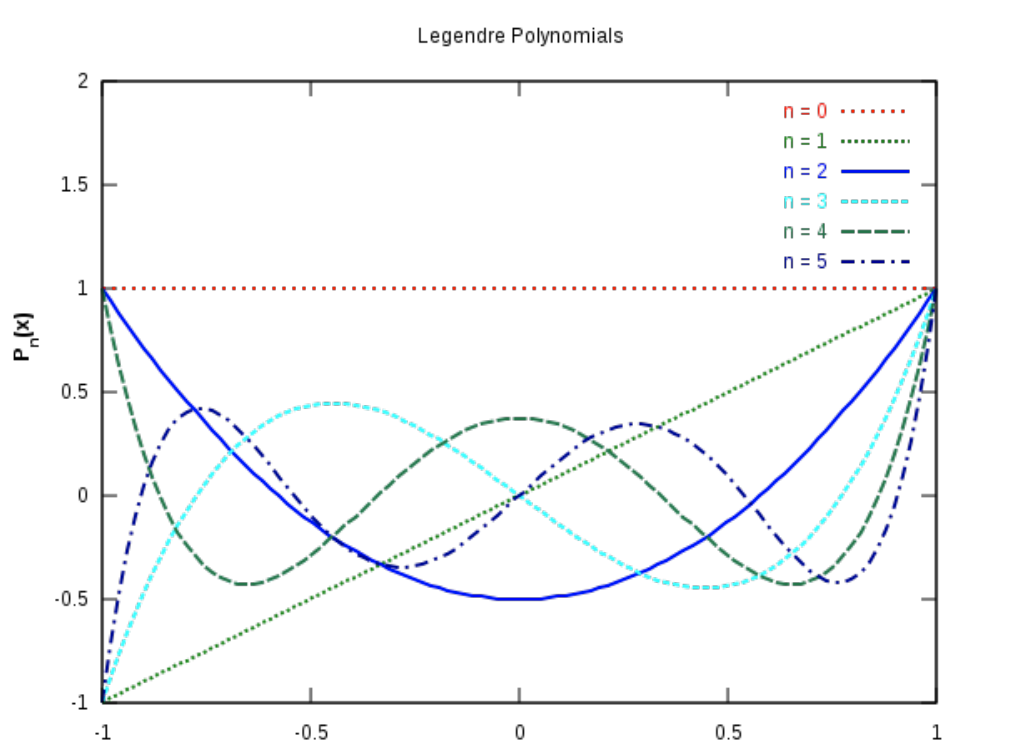
\includegraphics[scale = 0.5]{Algèbre linéàaire/Screenshot 2024-12-10 163537.png}
                
            \end{subparag}
            
        \end{parag}

        \begin{parag}{Matrice symétriques}
            \begin{definition}
                Une matrice carrée $A$ est \textcolor{red}{symétrique} si $A^T = A$
            \end{definition}
            \begin{subparag}{Exemple}
                La matrices diagonales sont symétrique, mais aussi les matrices de la forme $B^TB$ puisque le coefficient $(i, j)$ est $\vec{b_1}\cdot\vec{b_j} = \vec{b_j}\cdot \vec{b_i}$
            \end{subparag}
            \begin{theoreme}
                Soit $A$ une matrice symétrique soient $\vec{u}$ un vecteurs propre de $A$ pour la valeurs propre $\lambda$ et $\vec{v}$ un vecteurs propre de $A$ pour une autre valeurs propre $\mu$. Alors $\vec{u}$ et $\vec{v}$ sont orthogonaux
            \end{theoreme}
            \begin{subparag}{Preuve}
                On doit montrer que $\vec{u}\cdot \vec{v} = 0$.
                \\
                L'astuce est de calculer $\lambda\cdot(\vec{u}\cdot\vec{v}) = \lambda \vec{u}\cdot\vec{v} = A\vec{u}\cdot\vec{v} = (A\vec{u})^T\vec{u} = (\vec{u}^TA^T)\vec{v} = \vec{u}^TA\vec{v} = \vec{u}\cdot A\vec{v} = \vec{u}\cdot\mu\vec{v} = \mu(\vec{u}\cdot\vec{v})$ 
                \\
                Conclusion, comme $\lambda \neq \mu$, $\vec{u}\cdot\vec{v} = 0$
                \\
                \begin{framedremark}
                    \textbf{Attention}
                Si $\lambda = \mu$, ce raisonnement ne fonctionne pas, le résultat est faux en général
                \end{framedremark}
            \end{subparag}
            \begin{subparag}{Exemple}
                La matrice $A = \begin{pmatrix}
                    1 & 2\\
                    2 & 1
                \end{pmatrix}$ est symétrique. On calcule
                \[c_A(t) = (t-3)(t+1) \text{ et } E_3 = Vect\left\{\begin{pmatrix}
                    1 \\ 1
                \end{pmatrix}\right\} \text{ et } E_{-1} = Vect\left\{\begin{pmatrix}
                    -1 \\ 1
                \end{pmatrix}\right\}\]
                \\
                On sait alors par la preuve faite au dessus. que $E_3 \perp E_1$. En normalisant les vecteurs propres on obtient une base orthonormée $\bmath = \left(\begin{pmatrix}
                    \sqrt{2}/2 \\ \sqrt{2}/2
                \end{pmatrix}, \begin{pmatrix}
                    -\sqrt{2}/2 \\ \sqrt{2}/2
                \end{pmatrix}\right)$ la matrice $(Id)_\bmath^{\cmath an} = \begin{pmatrix}
                    \sqrt{2}/2 & -\sqrt{2}/2 \\
                    \sqrt{2}/2 & \sqrt{2}/2
                \end{pmatrix} = U$ est orthogonale.
                \\
                Et donc $(Id)_{\cmath an}^\bmath = U^T$ et $U^TAU = \begin{pmatrix}
                    3 & 0 \\ 0 & -1
                \end{pmatrix}$
            \end{subparag}
        \end{parag}
        \begin{parag}{Orthodiagonalisation}
            \begin{definition}
                Une matrice carrle $A$ est \textcolor{red}{diagonalisable par un changement de base orthonormée} ou \textcolor{red}{orthodiagonalisable} s'il existe une matrice $P$ orthogonale telle que $P^TAp$ est diagonale.
            \end{definition}
            \begin{theoreme}
                Une matrice $A$ est orthodiagonalisable si et seulement si elle est symmétrique
            \end{theoreme}
        \end{parag}
        \begin{parag}{Théorème spectral}
            \begin{theoreme}
                Soit $A$ une matrice symétrique. Alors
                \begin{enumerate}
                    \item A admet $n$ valeurs propres réelles, compte tenu de leur multiplicité
                    \item Pour toute valeurs propres $\lambda$ on a $mult(\lambda) = \dim E_\lambda$
                    \item Si $\lambda \neq \mu$ alors $E_\lambda \perp E_\mu$
                    \item $A$ est orthodiagonalisable
                \end{enumerate}
            \end{theoreme}
        \end{parag}
\lecture{26}{2024-12-12}{Dernier cours peut être?}{}

\begin{parag}{Suite}

    
\begin{framedremark}
    Si $\lambda$ est une valeurs propre de multiplicité $\geq 2$, alors la base de vecteurs prorpres de $E_\lambda$ fournie par la méthode de Gauss n'est pas orthogonale en général, il faut \textcolor{red}{Gram-Schmidter} pour obtenir une base orthonormée de vecteurs propres.
\end{framedremark}
\begin{subparag}{Exemple}
    \[A = \begin{pmatrix}
        4 & 1 & 3 & 1\\
        1 & 4 & 1 & 3\\
        3 & 1 & 4 & 1\\
        1 & 3 & 1 & 4
    \end{pmatrix}\]
    On cherche $c_A(t)$ :
    \begin{align*}
        (1-t)^2\begin{vmatrix}
            4-t & 1 & 3 & 1\\
            1 & 4-t & 1 & 3\\
            0 & -1 & 0 & 1
        \end{vmatrix} &= (1-t)^2\cdot1\begin{pmatrix}
            7-t & 2 & 1\\
            2 & 7-t & 3\\
            0 & 0 & 1
        \end{pmatrix}\\ 
        &= (1-t)^2\begin{vmatrix}
            7-t  & 2\\
            2 & 7-z
        \end{vmatrix} \\
        &= (1-t)^2(t^2 - 14t + 45)\\
        &= (1-t)^2(t-5)(t-9)
    \end{align*}
    On a donc trois valeurs propres 5, 9 et 1. avec $mult(1) = 2$.
    \\
    On peut maintenant trouver les espaces propres:
\begin{align*}
    E_5 = Vect\left\{\begin{pmatrix}
        -1/2\\
        1/2 \\ -1/2 \\ 1/2
    \end{pmatrix}\right\} \; \; \; \; E_9 = Vect\left\{\begin{pmatrix}
        1/2\\1/2\\1/2\\1/2
    \end{pmatrix}\right\} 
\end{align*}
On verifie ensuite $E_5 \perp E_9$.\\
On doit encore calculer $E_1$ et trouver une base orthonormée de $E_1$ pour orthodiagonaliser $A$.
\begin{align*}
    E_1 &= \ker(A - I_4) = \ker\begin{pmatrix}
        3 & 1 & 3 & 1\\
        1 & 3 & 1 & 3\\
        3 & 1 & 3 & 1\\
        1 & 3 & 1 & 3
    \end{pmatrix}\\
    &= \ker \begin{pmatrix}
        3 & 1 & 3 & 1\\
        1 & 3 & 1 & 3\\
        0 & 0& 0 & 0\\
        0 & 0& 0 & 0
    \end{pmatrix}\\
    &= \ker\begin{pmatrix}
        0 & -8 & 0 & -8\\
        1 & 3 & 1 &3\\ 
        que & des & 0
    \end{pmatrix} = \ker\begin{pmatrix}
        0 & 1 & 0 & 1\\
        1 & 0 & 1 & 0
    \end{pmatrix}
\end{align*}
Ce qui nous donne que base:
\begin{align*}
    Vect\left\{\begin{pmatrix}
        -1 \\ 0 \\ 1 \\ 0
    \end{pmatrix}, \begin{pmatrix}
        0 \\ -1 \\ 0 \\ 1
    \end{pmatrix}\right\} = Vect\left\{\begin{pmatrix}
        -\sqrt{2}/2\\
        0 \\
        \sqrt{2}/2\\
        0
    \end{pmatrix}, \begin{pmatrix}
        0 \\ -\sqrt{2}/2\\ 0 \\ \sqrt{2}/2
    \end{pmatrix}\right\}
\end{align*}
On obtient une base orthonormée de vecteurs propres:
$\bmath = \left(\begin{pmatrix}
        -\sqrt{2}/2\\
        0 \\
        \sqrt{2}/2\\
        0
    \end{pmatrix}, \begin{pmatrix}
        0 \\ -\sqrt{2}/2\\ 0 \\ \sqrt{2}/2
    \end{pmatrix}, \begin{pmatrix}
        -1/2\\
        1/2 \\ -1/2 \\ 1/2
    \end{pmatrix}, \begin{pmatrix}
        1/2\\1/2\\1/2\\1/2
    \end{pmatrix}\right)$
    \\
    \[U = \begin{pmatrix}
        -\sqrt{2}/2 & 0 & -1/2 & 1/2\\
        0 & -\sqrt{2}/2 & 1/2 & 1/2\\
        \sqrt{2}/2 & 0 & -1/2 & 1/2\\
        0 & \sqrt{2}/2 & 1/2 & 1/2
    \end{pmatrix}\]
    On trouve donc:
    \\
    $U^{-1} = U^T$ et $U^T AU = diag(1, 1, 5, 9)$
    \begin{framedremark}
        Le but ici c'est de trouver une base qui est orthonormée et donc lorsqu'on trouve la base qui est $U$ on peut faire un changement de base et c'est la formule de base $P^{-1}AP = B$ où $B$ est la matrice dans la base changée qui est donc une diagonale.
    \end{framedremark}
\end{subparag}
\end{parag}
\begin{parag}{Méthode}
\begin{enumerate}
    \item Vérifie que $A$ est symétrique
    \item Calculer $c_A(t)$ et en extraire les racines (valeurs propres)
    \item Calculer les espaces propres pour chacun, le procédé de Gram-Schmidt donne une base orthonormée.
    \item En assem blant les base des espaces propres on obtient une base orthonormée $\mathcal{U}$ de $\mathbb{R}^n$
    \item La matrice $P$ dont les colonnes sont les vectteurs $\vec{u}_i$ de $\mathcal{U}$ est orthogonale et $P^TAP$ est diagonale
\end{enumerate}   
\begin{framedremark}
    L'avantage ici c'est que l'inverse de la matrice de changement de base est juste sa transposée
\end{framedremark}
\end{parag}
\begin{parag}{Matrice de projection}
    Soit $\vec{u}$ un vecteurs unitaire et $A = \vec{u}\vec{u}^T$. Alors
    \begin{formule}
        \[A\vec{x} = \vec{u}(\vec{u}^T\vec{x}) = (\vec{u}\cdot\vec{x})\vec{u}\]
    \end{formule}
    \begin{enumerate}
        \item $\vec{u}$ est un vecteur propre de $A$ pour la valeur propre $1$ car $(\vec{u}\cdot\vec{u})\vec{u} = \vec{u}$
        \item Posons $W = Vect(\vec{u})$. Alors $W^\perp$ est le noyau de $A$
        \item Ainsi $E_1 = W$ et $E_0 = W^\perp$
    \end{enumerate}
    \begin{subparag}{Proposition}
        La matrice $A = \vec{u}\vec{u}^T$ est la matrice de la projection orthogonale sur $W = Vect(\vec{u}).$ On a $A\vec{x} = \text{proj}_\vec{u}\vec{x}$
    \end{subparag}
    C'est un cas particulier que nous avons vu pour $UU^T$, matrice de projection orthogonale quand les colonnes de $U$ sont orthonormées.
    \begin{subparag}{Exemple}
        \begin{enumerate}
            \item $\vec{u} = \begin{pmatrix}
                1 \\ 0
            \end{pmatrix}$ Alors $\vec{u}\vec{u}^T = \begin{pmatrix}
                1 & 0 \\ 0 & 0
            \end{pmatrix}$ qui est une projection orthognonale sur $Ox$.
            \item $\vec{u} = \begin{pmatrix}
                \sqrt{2}/2\\ \sqrt{2}/2
            \end{pmatrix}$ Alors $\vec{u}\vec{u}^T = \begin{pmatrix}
                1/2 & 1/2\\ 1/2 & 1/2
            \end{pmatrix}$ qui est une projection orthogonal sur l'axe $x = y$
            \item $\vec{u} = \begin{pmatrix}
                1 \\ 1
            \end{pmatrix}$ Alors $\vec{u}\vec{u}^T = \begin{pmatrix}
                1 & 1\\ 1 & 1
            \end{pmatrix}$ qui n'est pas une matrice de projection
        \end{enumerate}
        C'est en fait même la projection de $(2)$ suivie d'une homothétie de rapport $2$.
    \end{subparag}
\end{parag}
\begin{parag}{Décomposition spectrale}
    \begin{definition}
        Soit $A$ symétrique, $U$ orthogonale et $U^TAU = D$ diagonale. L'ensemble des valeurs propres de $A$ est appelé \textcolor{red}{spectre} de $A$
    \end{definition}
    On prends $A =UDU^T = (\vec{u}_1, \vec{u}_2, \dots, \vec{u}_n)\begin{pmatrix}
        \lambda_1 & 0 & \cdots & 0\\
        0 & \lambda_2 & 0 & 0\\
        \vdots & \ddots & \ddots & 0\\
        0 & \cdots & 0 & \lambda_n
    \end{pmatrix}\begin{pmatrix}
        \vec{u}_1^T\\ \vec{u_2}^T\\
        \vdots \\
        \vec{u_n}^T
    \end{pmatrix}$
    \\
    $= (\lambda_1\vec{u}_1\dots\lambda_n\vec{u}_n)\begin{pmatrix}
        \vec{u}_1^T\\ \vec{u_2}^T\\
        \vdots \\
        \vec{u_n}^T
    \end{pmatrix} = \lambda_1\vec{u_1}\vec{u_1}^T + \cdots + \lambda_n\vec{u}_n\vec{u_n}^T = A$ et qui est la décomposition spectrale.
    \begin{subparag}{exemple}
        Soit $A = \begin{pmatrix}
            1 & 2 \\ 2 & 1
        \end{pmatrix}$ la matrice symétrique que nous avons orthodiagonalisée mardi. Nous avonstrouve une base orthonormée de vecteurs propres (pour les valeurs propres -1 et 3):
        \[\mathcal{U} = (\vec{u_1}, \vec{u_2}) = \left(\begin{pmatrix}
            -\sqrt{2}/2 \\
            \sqrt{2}/2
        \end{pmatrix}, \begin{pmatrix}
            \sqrt{2}/2 \\ \sqrt{2}/2
        \end{pmatrix}\right)\]
        La décomposition spectrale de $A$ est donc
        \[A = -1\cdot\vec{u_1}\vec{u_1}^T + 3\cdot\vec{u}_2\vec{u}_2^T\]
    \end{subparag}
\end{parag}

\begin{parag}{La caractéristique d'un corps fini}
    Soit $K$ un corps fini (ayant un nombre fini d'éléments). Considérons l'ensemble de tous les multiples entiers de $1_K$ dans $K$, c'est à dire les éléments de la forme $n \times 1 = 1_K + \cdots + 1_K$.\\
    Comme $K$ est fini, $\{n\cdot 1_K| n \in \mathbb{Z}\}$ aussi est fini. Autrement dit, il existe des entiers n tels que $n \cdot 1_K = 0$ (si $m \cdot 1_k = m'\cdot 1_K$, alors $(m-m')\cdot 1_K = 0_K$)
    \begin{definition}
        Le plus petit entier non nul $n$ tel que $n\cdot 1_K = 0$ s'appelle la \textcolor{red}{caractéristique} de $K$ et on le not $carK$.
    \end{definition}
    \begin{theoreme}
        La caractéristique d'un corps fini $K$ est un nombre premier.
    \end{theoreme}
    \begin{framedremark}
        La caractéristique d'un corps est un nombre entiers, ce n'est \textbf{pas} un élément du corps.
    \end{framedremark}
    \begin{subparag}{Exemple}
        \begin{enumerate}
            \item $car\mathbb{F}_2 = 2$ et $\mathbb{F}_p = p$, premier
            \item $car\mathbb{F}_4 = 2$
            \item $car\mathbb{R} = 0$ $n\cdot1 \neq 0$
        \end{enumerate}
        \begin{lemme}
            Dans un corps $K$, si $x, y \neq 0$, alors $x\cdot y = 0$
        \end{lemme}
        \textbf{Preuve} On montre que si $x\cdot y = 0$, alors $x$ ou $y$ est nul. Supposons que l'un des deux est non nul, disons que c'est $x$. On doit prouver que $y = 0$.\\
        Comme $x \neq 0$, $x^{-1}$ existe Alors
        \[0 = x^{-1}\cdot 0 = x^{-1}(x\cdot y) = (x^{-1}x)y = 1_K\cdot y = y = 0\]
        Soit $K$ un corps fini et $n = car(K) \in \mathbb{N}^*$. On motre que si $n = a\cdot b$, alors $a$ ou $b$ $= 1$.
        \\
        Comme $n \neq 1$ car $1\cdot 1_K = 1_K \neq 0$, n sera donc premier.
        \\
        Ce qu'on sait dès le début c'est $0 = n\cdot 1_K = a\cdot b \cdot 1_K = 1_K + \cdots + 1_K = $ par distributivité $ = (1_K + \cdots + 1_K)\cdot (1_K + \cdots + 1_K)$ où la premier parenthèse est $a$ et la deuxième est $b$ on a alors $= (a\cdot 1_K)\cdot (b\cdot 1_K)$
        \\
        Par le lemme, soit $a\cdot 1_K = 0$, soit $b\cdot 1_K ) 9$. Or $n$ est le plus petit entier non nul tel que $n \cdot 1_K = 0$.
        \\
        Donc soit $a = n$ et $b = 1$, soit $b = n$ et $a = 1$.
    \end{subparag}
\end{parag}
\begin{parag}{La cardinalité d'un corps fini}
    Soit $p = \text{car}K$. Alors le corps $\mathbb{F}_p$ agit sur $K$ par multiplication
    \begin{definition}
        Soit $k \in \mathbb{F}_p$ et $x \in K$. On pose $k \cdot x = (k\cdot 1_K)\cdot x$
    \end{definition}
    Cette action est bien défini puisque $p\cdot 1_K = 0$. Les propriétés de l'action sont toutes conséquence du fait que $K$ est un corps.
    \begin{proposition}
        Soit $K$ un corps fini et $p = \text{car}K$. Alors $K$ est un $\mathbb{F}_p$-espace vectoriel.
    \end{proposition}
    \begin{theoreme}
        Soit $K$ un corps fini et $p = $car$K$. Alors il existe $n$ tel que $K$ a $p^n$ éléments. On appelle ce nombre la \textcolor{red}{cardinalité} de $K$. 
    \end{theoreme}
    \begin{subparag}{preuve}
        Si $K$ est fini, $\dim_{\mathbb{F}_p}K < \infty$ et on peut choisir une base $\bmath$ qui a $n$ éléments. Le passage en coordonées $()_\bmath : K \to (\mathbb{F}_p)^n$ tel que $x \to (x)_\bmath$
        \\
        Ce passage est une application bijective. Et donc commme vu en AICC, Le nombre d'élément de le domaine et le codomaine est le même. La cardinalité de $K$ est la même que celle de $(\mathbb{F}_p)^n$ et sa cardinalité vaut $p^n$.
    \end{subparag}
    \begin{subparag}{Exemple}
        \begin{itemize}
            \item $Card(\mathbb{F}_p) = p$
            \item  $Card(\mathbb{F}_4) = 2^2$
            \item $Card(K) = 6$ est impossible
        \end{itemize}
    \end{subparag}
\end{parag}

\begin{parag}{Construction de corps finis}
    La construction de $\mathbb{F}_4$ n'est pas isolé, la méthode générale fonctionne de la même manière. Soit $p$ un nombre premier.
    \begin{itemize}
        \item Trouver un polynôme $p(t)$ unitaire irréductible de degré $n$ dans $\mathbb{F}_p[t]$
        \item Considérer l'ensemble $K$ de tous les restes de division par $p(t)$. il y en a $p^n$
        \item Définir la somme dans $K$ comme dans $\mathbb{F}_p[t]$
        \item Défini le produit dans $K$ par celui de $\mathbb{F}_p[t]$, \textcolor{red}{modulo} $p(t)$
        \item Alors $K$ est un corps de cardinalité $p^n$
    \end{itemize}

    \begin{subparag}{Exemple : le corps $\mathbb{F}_{49}$}
        Nous cherchons un polynôme irréductible de degré $2$
        \begin{proposition}
            Soit $K$ un corps et $p(t) = t^2 - a$ si $a$ n'est pas un carré (dans $K$), alors $p(t)$ est irréductible.
        \end{proposition}
        \textbf{Preuve}
        En effet $p(t)$ est irreduvtible si et seulement si il n'a pas de racine (car il est de degré 2), si et seulement si $p(x) \neq 0$ pour tout $x \in K$.
        \\
        Or, $p(x) = x^2 - a = 0$ si et seulement si $a = x^2$ est un carré
        \begin{framedremark}
            Pour trouver un polynôme irréductible de degré $2$ à coefficients dans $\mathbb{F}_7$, nous cherchons à comprendre quels éléments sont des carrés.
        \end{framedremark}

            \begin{tabular}{c||c|c|c|c|c|c|c|}
                x &0 & 1 & 2 & 3 & 4 & 5 & 6 \\
                \hline
                 $x^2$& 0 & 1 & 4 & 2 & 2 & 4 & 1 
            \end{tabular}
            \\
            Par exemple $3$ n'est pas un carrl dans $\mathbb{F}_7$, donc $t^2-3$ est irréductible.
            \\
            $\mathbb{F}_{49}$ est l'ensemble des restes de la division par $t^2 - 3$ tel que
            \[ = \{a\cdot t + b | a, b \in \mathbb{F}_7\}\]
            \begin{itemize}
                \item Somme: $(3t + 2) + (3t + 5) = 6t + 7 = 6t = -t$
                \item Poroduit $(t+1)(t+4) = t^2 + 5t + 4 = 3 + 5t + 4 = 5t$ car on peut simplifer par $t^2 - 3$ on fait la division euclidienne par $t^2 - 3$ et on trouve $1$ et le reste $5t$.
                \\
                On pose $\alpha = [t]$ et comme $[t^2 - 3] = 0$ dans $\mathbb{F}_{49}$
                \[\mathbb{F}_{49} = \{a \cdot \alpha + b | a, b \in \mathbb{F}_7\}\]
                le produit est déterminé par $\alpha^2 = 3$
            \end{itemize}
    \end{subparag}
\end{parag}
\textbf{Résume court}
\lecture{1}{2024-01-01}{Résumé du court}{}
On voit juste mettre les formule et les trucs à savoir vite fait.\\
\begin{parag}{Déterminant}
    \begin{subparag}{Opération élémentaire}
        Application des opération élémentaire sur le déterminant:
        \begin{itemize}
            \item Type I: Interchanger des lignes entre elle ne change pas le determinant
            \item Type II: changer le signe de la matrice change le signe du déterminant
            \item Type III: En mutlipliant une ligne par un scalaire $\alpha \in \mathbb{R}$, le déterminant est aussi multiplier par ce scalaire.
        \end{itemize}
    \end{subparag}
    Soit une matrice $A$, 
    \begin{truc}
        Si une ligne de $A$ est combinaison linéaire des autres lignes, alors $\det A = 0$
    \end{truc}
    \begin{theoreme}
        \begin{itemize}
            \item $\det (A^t) = \det A$
            \item $\det(AB) = \det A \cdot \det B$
            \item Si $A$ est inversible, alors $\det(A^{-1}) = \frac{1}{\det(A)}$
        \end{itemize}
    \end{theoreme}
    
\end{parag}
\begin{parag}{Famille génératrice}
    Soit $W$ un sous espace vectoriel de $V$.
    \begin{itemize}
        \item Le sous espace $W = Vec(v_1, \dots, v_k)$ est le sous espace engendré par les vecteurs $v_1, \dots, v_k$
        \item Les vecteurs $v_1, \dots, v_k$ sont les générateurs de $W$
        \item L'ensemble $\{v_1, \dots, v_k\}$ forme une \textbf{partie génératrice} de $W$
    \end{itemize}
    \begin{subparag}{Extraire des bases etc...}
        \begin{theoreme}
            Si l'un des vecteurs $v_i$ est combinaison linéaire des autres, alors la famille obtenue en supprimant $v_i$ engendre encore $V$.
            si $V \neq \{0\}$, il existe une sous famille de $\{v_1, \dots, v_k\}$ qui forme une base de $V$.
        \end{theoreme}
    \end{subparag}
    \begin{subparag}{Cardinalité d'une base}
    Soit:
    \begin{itemize}
        \item $V$ un espace vectoriel
        \item $\bmath = (b_1, \dots, b_n)$ une base de $V$
        \item $\cmath = (c_1, \dots, c_n)$ une famille ordonnée de vecteurs de $V$
    \end{itemize}
    \begin{theoreme}
        La famille ordonnée de $\cmath$ est une base de $V$ si et seulement si la matrice $A = ((c_1)_\bmath, \dots, (c_m)_\bmath)$ a un pivot dans chaque ligne et chaque colonne.
    \end{theoreme}
    \begin{framedremark}
        Cela ce "marie" très bien avec une matrice carré et inversible qui rejoint tout ensemble
    \end{framedremark}
        
    \end{subparag}
    \begin{theoreme}{de la base incomplète}
        Soit $V$ un espace vectoriel de dimension $n$ et $\{e_1, \dots, e_k\}$ une famille libre de vecteurs de $V$. Il existe alors des vecteurs $e_{k+1}, \dots, e_n$ tels que $(e_1, \dots, e_n)$ forme une base de $V$.
    \end{theoreme}
    \begin{truc}
        On utilise les parenthèse pour une base et des acollades pour les familles de vecteurs§
    \end{truc}
\end{parag}
\begin{parag}{Décomposition $LU$}
    Le but est d'avoir une matrice triangulaire inferieur ($L$) et une supérieur:
    \begin{itemize}
        \item $U$ est juste la matrie échelonnée (on s'arrête en bas)
        \item $L$ est la matrice qui comment à $I_n$ et on fait l'opposé des opération faite sur la matrice (si on ajoute $1/2$ a une ligne, on enlève $1/2$ sur la colonne du même indice)
        \item $A = LU$
    \end{itemize}
\end{parag}
\begin{parag}{Inverse de matrices et déterminants}
    L'inverse d'une matrice est donné par:
    \[A^{-1} = \frac{1}{\det A}(Com A)^t\]
    
\end{parag}


\begin{parag}{Indépendance linéaire}
    \begin{truc}
        Des vecteurs sont linéairement indépendants lorsque la seule solution de l'équation:
        \[\alpha_1v_1 + \cdots + \alpha_n v_n = 0\]
        Est:
        \[\alpha_1 = \alpha_2 + \cdots + \alpha_n = 0\]
        On voit que c'est le même principe que lorsqu’on cherche le noyau, on prend la matrice dans une base (canonique c'est souvent plus simple) et on échelonne. et s'il y a moins de colonnes pivots que de colonnes, alors les vecteurs sont dépendants.
        
    \end{truc}
    \begin{truc}
        Si la matrice des vecteurs est carrée, on peut faire le déterminant et voir si il est égal à 0.
    \end{truc}
    
    
\end{parag}


\begin{parag}{Injectivité}
    Il y a plein de propriétés lorsqu'une matrice est injective:
    \begin{truc}
        \begin{itemize}
            \item Une seul solution et elle est trivial pour $A\vec{x} = \vec{0}$
            \item $\ker A = \{0\}$
            \item Les colonnes sont linéairement indépendantes
        \end{itemize}
        Si la matrice est carrée et de taille $n \times n$:
        \begin{itemize}
            \item La matrice $A$ est inversible
            \item $\det A \neq 0$
            \item Les colonnes de $A$ forment une base de \R$^n$
            \item $Im\; A = n$
            \item $\ker A = \{0\}$
            \item $dim\; Ker\; A = 0$
        \end{itemize}
    \end{truc}
    On voit que si une application est injective, a vraiment beaucoup de propriétés qui en ressort.
\end{parag}

\begin{parag}{Surjectivité}
    \begin{truc}
        Une application $f : V \to W$ entre deux espaces vectoriels $V$ et $W$ est dite surjective si pour chaque vecteur $w \in W$, il existe au moins un vecteur $v \in V$ tel que $f(v) = w$.
    \end{truc}
     En d'autres termes, l'image de $f$ couvre tout l'espace $W$.
    \\
    Si $f$  est surjective, alors:
    \begin{truc}
        \[dim\; Imf = dim\; W\]
    \end{truc}  
    Donc, pour qu'une application soit surjective, le rang de $f$ doit être égal à la dimension de l'espace \textbf{d'arrivée} $W$.
    \begin{itemize}
        \item Cas où $dim\;V \> dim\;W$:
        \\
        Dans ce cas il est possible pour $f$ d'être surjective
        \item Cas où $dim\;V = dim\;W$
        Dans ce cas, la dimension du noyau de $f$ doit être égal à $0$. 
        \item Cas où $dim \; V < dim\; W$
        \\
        Dans ce cas, il est impossible que $f$ soit surjective.
    \end{itemize}
    \begin{truc}
        Si une application est surjective Alors:
        \[A^T\vec{y} = \vec{0} \text{ Possède une solution unique}\]
        
    \end{truc}
\end{parag}

\begin{parag}{Bijectivité}
    Une bijection est une application qui est injective et surjective en même temps.
    \begin{definition}
        Une application linéaire bijective est appelée \textcolor{red}{isomorphisme}
    \end{definition}
\end{parag}
\begin{parag}{Application linéaire}
    \begin{truc}
        Soit $T$ une application linéaire. Alors:
        \[T(\alpha u + \beta v) = \alpha T(u) + \beta T(v)\]
        \[T(0) = 0\]
    \end{truc}
\end{parag}

\begin{parag}{Espace vectoriel}
    C'est le même principe que l'application linéaire:
    \begin{itemize}
        \item \textbf{L'addition}, si on prend deux vecteur de $V$ et qu'on les additions, ils doivent rester dans $V$.
        \item Si on multiplie par un réel un vecteur de $V$, il doit rester dans $V$.
    \end{itemize}
    
\end{parag}


\begin{parag}{Noyau}
    \begin{truc}
        Le noyau est la solution générale du système homogène.
        \[A\vec{x} = \vec{0} \]
    \end{truc}
    \begin{truc}
        Le noyau appartient à l'espace de départ 
    \end{truc}
\end{parag}
    
\begin{parag}{Image}
    L'image est tout ce qui peut être comme résultats de l'application.\\
    Elle généralise la notion de sous-espace $ColA$ engendré par les colonnes d'une matrice $A$.
    \begin{truc}
        L'image appartient à l'espace d'arrivée.
    \end{truc}
    \begin{truc}
        L'image d'une application linéaire $T: v \to W$ est le sous-ensemble $ImT = \{ w \in W| \text{ il existe } v \in V \text{ tel que } Tv = w\}$.
    \end{truc}
    
\end{parag}

\begin{parag}{Espace-colonne, Espaces-lignes}
    \begin{truc}
        L'espace colonne est l'espace engendré par les colonnes de $A$, donc ce sont les vecteurs où il y a des colonnes pivots.
    \end{truc}
    \begin{truc}
        L'espace ligne est l'espace engendré par les lignes de $A$ qui ont un pivot. Pour donner l'espace ligne, on met les lignes où il y a un pivot et on les réécrit en vecteur (en colonne).
    \end{truc}
    \begin{truc}
        \[dim\; ColA = dim\; LgnA\]
    \end{truc}
    Pourquoi ça marche:
    \begin{itemize}
        \item Le nombre de lignes linéairement indépendantes est égal au nombre de lignes contenant un pivot
        \item Le nombre de colonnes linéairement indépendantes est égal au nombre de colonnes contenant un pivot.
    \end{itemize}
\end{parag}

\begin{parag}{Théorème du rang}
Soit $T: V \to W$ Une application linéaire en espaces vectoriels de dimensions finies.
    \begin{truc} 
        le rang est la dimension de l'image
    \end{truc}
    \begin{truc}
        \begin{formule}
            \[\rang\; T + dim\; KerT = dim\; V\]
        \end{formule}
    \end{truc}
    que la dimension de l'image et la dimension du noyau ensemble sont égales à la dimension de l'ensemble de départ.\\
    C'est fort parce que l'image de base réside donc l'espace d'arrivée donc on arrive grâce à ce théorème à relier l'image à l'espace de départ. 
    \\
    Grâce à ce théorème on peut vraiment vraiment rapidement trouver plusieurs dimensions avec la matrice d'application de taille $n \times m$.
    \begin{itemize}
        \item $dim\; KerA = $nombre de colonnes sans pivot
        \item $dim\; ImA = \text{rang}A = $ nombre de colonnes-pivot
        \item nombre de colonnes-pivot + colonnes sans pivot $= n$.
    \end{itemize}
\end{parag}

\begin{parag}{Changement de base}
    Si on veut passer de la base $\mathcal{B}$ à la base $\mathcal{C}$ on a le théorème:
    \begin{truc}
        \[(Id_V)_{\mathcal{B}}^\mathcal{C}(v)_{\mathcal{B}} = (v)_{\mathcal{V}}\]
    \end{truc}
    \begin{theoreme}
        \[(T)_\bmath^\cmath (v)_\bmath = (Tv)_\cmath\]
    \end{theoreme}
    Donc ici $Id_V$ est la matrice de changement de base. En gros. on a le vecteur $v$ exprimé dans la base $\mathcal{B}$ et ensuite le vecteur $v$ exprimé dans la base $\mathcal{C}$.
    \begin{truc}
        La matrice de changement de base $(Id_V)_{\mathcal{B}}^\mathcal{C}$ est construite en écrivant les vecteurs de la base $\mathcal{B}$ en fonction de la base $\mathcal{C}$\\
        En exprimant chaque $b_i$ en fonction de $c_j$ on obtient la matrice $(Id_V)_{\mathcal{B}}^\mathcal{C}$.
    \end{truc}
    \begin{truc}
        Soit $\mathcal{B}$ et $\mathcal{C}$ deux bases de l'espace vectoriel de \R$^n$.\\
        Soit $P = (Id)_{\mathcal{B}}^{\mathcal{C}}$ la matrice de changement de base de $\mathcal{B}$ vers $\mathcal{C}$.
        \begin{itemize}
            \item La matrice $P$ est inversible
            \item la matrice inverse $p^{-1}$ est une matrice de changement de base de $\mathcal{C}$ vers $\mathcal{B}$.
            \item Toute matrice inversible de taille $n \times n$ est une matrice de changement de base,
        \end{itemize}
    \end{truc}
    \begin{definition}
        Deux matrices carrées $A$ et $B$ de taille $n \times n$ sont \textcolor{red}{semblables} s'il existe une matrice inversible $P$ de taille $n \times n$ telle que 
        \begin{formule}
            \[A = P^{-1}BP\]
        \end{formule}
    \end{definition}
    \begin{truc}
        Deux matrice semblables ont le même polynôme caractéristique
    \end{truc}
    \begin{subparag}{les relations $\sim$ et $\approx$}
    \begin{definition}
        Les matrices $A$ et $B$ sont équivalentes selon les lignes et les colonnes s'il existe des opérations élémentaires sur les lignes et les colonnes qui transforment $A$ en $B$. Il existe dont deux matrices inversible $P$ et $Q$ telle que:
        \[PAQ = B\]
        On le note
        \[A \sim B\]
    \end{definition}
    \begin{truc}
    \[A \approx B \implies A \sim B\]
    \end{truc}
        
    \end{subparag}
\end{parag}
\begin{parag}{Diagonalisation}
    \begin{theoreme}
        Une matrice $A$ de taille $n \times n$ est diagonalisable si et seulement s'il existe une base $\bmath$ de $\mathbb{R}^n$ formée de vecteurs propres de $A$
    \end{theoreme}
    \begin{truc}
        Si la somme des coefficients de chaque lignes est égal à $\phi$ alors $\phi$ est une valeur propre et $\begin{pmatrix}
            \phi \\ \phi \\ \phi
        \end{pmatrix}$ est un vecteur propre
    \end{truc}
    \begin{truc}
        Si $A - \phi I_n = \begin{pmatrix}
            \phi & \phi & \phi\\
            \phi & \phi & \phi\\
            \phi & \phi & \phi
        \end{pmatrix}$ alors par exemple ici le rang est $1$ et la $\dim \ker = 2$ est donc on sait que l'espace propre est $2$ et que $\phi$ est valeur propre
    \end{truc}
    \begin{theoreme}
        Soit $A$ une matrice de taille $n \times n$ ayant $n$ valeurs propres distinctes. Alors $A$ est diagonalisable
    \end{theoreme}

    \begin{truc}
        Soit $\lambda$ une valeur propre de $A$, alors $1 \leq \dim E_\lambda \leq mult(\lambda)$
    \end{truc}
    \begin{truc}
        Soit $A$ pas inversible alors $\ker A \neq \{\vec{0}\}$ et donc $0$ est valeur propre de $A$ et donc \\
        \begin{itemize}
            \item $c_A(0) =0$\\
            \item $c_A(t)$ a coefficient constant nul
            \item $t$ divise $c_A(t)$
        \end{itemize}
    \end{truc}
    \begin{subparag}{Critère de diagonalisation}
        Une matrice $A$ est diagonalisable (sur $\mathbb{R}$) si et seulement si:
        \begin{enumerate}
            \item Le polynôme caractéristique est \textcolor{red}{scindé}: il se décompose en produit de facteur $(\lambda - t)$ avec $\lambda \in \mathbb{R}$
            \item Pour tout $\lambda$, on a $\dim E_\lambda = mult(\lambda)$
        \end{enumerate}
        Si $A$ est diagonalisable, on forme une base de vecteurs propres en réunissant les vecteurs de base de chaque espace propre.
    \end{subparag}
    \begin{subparag}{Méthode de diagonalisation}
        Soit $T: V \to V$ une application linéaire
        \begin{enumerate}
            \item Choirsir une base $\cmath$ de $V$ (la base canonique si elle existe)
            \item Ecrire la matrice $A = (T)_\cmath^\cmath$ de $T$ dans cette base
            \item Calculer le polynôme caractérsitque $c_a(t)$
            \item Si $c_A(t)$ n'est pas scindé, $A$ n'est pas \textcolor{red}{diagonalisable}.
            \item $c_A(t)$ est scindé, extraire les racines de $\lambda$ de $c_a(t)$ et calculer les multiplicité algébrique
            \item Calculer les espaces propres $E_\lambda$ et les multiplicités géométriques
            \item Si $\dim E_\lambda = mult(\lambda)$ pour une valeur propre $\lambda$, alors $A$ n'est pas \textcolor{red}{diagonalisable}
            \item Si $\dim E_\lambda = mult(\lambda)$ pour tout $\lambda$, alors $A$ est \textcolor{green}{diagonalisable}
        \end{enumerate}
        Dès lors
        \begin{enumerate}
            \item Soit $T: V \to V$ une application linéaire \textcolor{green}{diagonalisable}
            Choisir une base $\bmath_\lambda$ de $E_\lambda$ pour toute valeurs de $\lambda$
            \item Réunir les $\bmath_\lambda$ pour former une base $\bmath$ de $V$
            \item $D = (T)_\bmath^\bmath$ est diagonale. Les valeurs propres apparaissent dans la diagonale dans l'ordre choisi pour contruire la base $\bmath$
            \item Les colonnes de la matrice de changement de base $P = (Id)_\bmath^\cmath$ sont les vecteurs de $\bmath$ exprimés en coordonnées dans $\cmath$
            \item Les colonnes de la matrice de changement de base $P = (Id)_\bmath^\cmath$ sont les vecteurs de $\bmath$ exprimés en coordonnées dans $\cmath$:
        \end{enumerate}
    \end{subparag}
    \begin{truc}
        Soit $A$ une matrice de taille $n \times n$. Alors $(-1)^{n-1}TrA$ est le coefficient de $t^{n-1}$ de $c_A(t)$ et $\det A$ est le coefficient constant
    \end{truc}
    \begin{truc}
        Si $A$ est diagonalisable, alors la trace de $A$ est égal à la somme des valeurs propres
    \end{truc}
\end{parag}

\begin{parag}{Orthogonalisation}
    \begin{subparag}{Produit scalaire}
    \begin{definition}{Produit scalaire}
        Soit $\vec{u}, \vec{v}$ deux vecteurs de $\mathbb{R}^n$. Le produit scalaire est:
        \begin{formule}
            \[\vec{u}\cdot \vec{v} = \vec{u}\vec{v} = u_1v_1 + \cdots + u_nv_n\]
        \end{formule}
    \end{definition}
    \textbf{Propriétés}
    \begin{itemize}
        \item Commutativité
        \item Distributivité
        \item Compataibilité avec l'action scalaire
        \item Positivité $\vec{u}\cdot \vec{u} \geq 0$ et $\vec{u}\cdot \vec{u} = 0 \Leftrightarrow \vec{u} = \vec{0}$
    \end{itemize}
        
    \end{subparag}
    \begin{definition}
     Une famille $(\vec{u}_1, \dots, \vec{u}_k)$ de vecteurs $\mathbb{R}^n$ est \textcolor{red}{orthogonale} si $\vec{u}_i \perp \vec{u_j}$ pour tout $i \neq j$. Cette famille est orthonormée si de plus $||\vec{u}_i|| = 1$ pour tout $i$.
    \end{definition}
    \begin{theoreme}
        Les colonnes d'une matrice $U$ de taille $m \times n$ sont orthogonales si et seulement si $U^TU = I_n$
    \end{theoreme}
    \begin{theoreme}
        Soit $U$ la matrice dont les colonnes sont les vecteurs $\vec{u_1}, \dots, \vec{u_k}$ d'une base \textcolor{red}{orthonormée} de $W$. Alors
        \begin{formule}
            \[proj_W\vec{y} = UU^T\vec{y}\]
        \end{formule}
    \end{theoreme}
    \begin{subparag}{Approximation quadratique}
        La distance minimale entre un vecteur $\vec{y}$ et un sous espace $W$ de $\mathbb{R}^n$ est réalisée par $\vec{z} = \vec{y} - proj\vec{y}$
        \begin{theoreme}
            Pour tout $\vec{w}\in W$ on a $||\vec{y} - \vec{w}|| \geq || \vec{y} - proj_W\vec{y}||$
        \end{theoreme}
        On note $\hat{y}$ la meilleur approximation quadratique de $\vec{y}$ dans $W$.
    \end{subparag}
    \begin{truc}
        Une famille orthogonale de vecteurs non nuls est libres
    \end{truc}
    \begin{truc}
        Soit $\{\vec{u}_1, \dots, \vec{u}_k\}$ une famille orthogonale de vecteurs non nuls de $\mathbb{R}^n$ et $U = (\vec{u}_1, \dots,\vec{u}_k)$ la matrice de taille $n\times k$ associée Alors:
        \begin{itemize}
            \item $U^TU$ est une matrice diagonale
        \end{itemize}
        Si la famille est orthonormée:
        \begin{itemize}
            \item $U^TU= I_k$
            \item $UU^T$ est une projection orthogonale sur $ImA$
        \end{itemize}
    \end{truc}
\begin{enumerate}
    \item Vérifie que $A$ est symétrique
    \item Calculer $c_A(t)$ et en extraire les racines (valeurs propres)
    \item Calculer les espaces propres pour chacun, le procédé de Gram-Schmidt donne une base orthonormée.
    \item En assemblant les base des espaces propres on obtient une base orthonormée $\mathcal{U}$ de $\mathbb{R}^n$
    \item La matrice $P$ dont les colonnes sont les vecteurs $\vec{u}_i$ de $\mathcal{U}$ est orthogonale et $P^TAP$ est diagonale
\end{enumerate}   
\begin{framedremark}
    L'avantage ici c'est que l'inverse de la matrice de changement de base est juste sa transposée
\end{framedremark}
\end{parag}

\begin{parag}{Méthode des moindres carrés}
La meilleurs solution possible d'une système incompatible tel que $A\vec{x} = \vec{b}$ où $A$ est une matrice $m \times n$.
    \begin{definition}
        Une vecteur $\hat{x} \in \mathbb{R}^n$ est une \textcolor{red}{solution au sens des moindres carrés} pour le système $A\vec{x} = \vec{b}$ si, pour tout $\vec{x} \in \mathbb{R}^n$
        \begin{formule}
            \[||\vec{b} - A\hat{x}|| \leq || \vec{b} - A\vec{x}||\]
        \end{formule}
    \end{definition}
    \begin{truc}
        Comme $A\vec{x} \in ImA$, le système est incomptabile si $b \notin ImA$. Le vecteur le plus proche de $\vec{b}$ dans $ImA$ est sa projection orthogonale.
        \begin{formule}
            \[\hat{b} = \text{proj}_{ImA}\vec{b}\]
        \end{formule}
    \end{truc}
    \begin{subparag}{Equation normale}
        \begin{theoreme}
            L'ensemble des solutions $A\vec{x} = \vec{b}$ au sens des moindres carrés est égal à l'ensemble non-vide des solutions de l'\textcolor{red}{équation normale} : 
            \begin{formule}
                $A^TA\hat{x} = A^T\vec{b}$
            \end{formule}
        \end{theoreme}
        \begin{truc}
            La norme du vecteurs $\vec{b} - A\hat{x}$ est appelée \textcolor{red}{écart quadratique}
        \end{truc}
        \begin{theoreme}
            La solution $\hat{x}$ au sens des moindres carrées est unique si et seulement si les colonnes de $A$ sont libres, ce qui est équivalent à exiger que la matrice $A^TA$ est inversible
        \end{theoreme}
    \end{subparag}
\end{parag}

\begin{parag}{Régression linéaire}
    \begin{enumerate}
        \item On représente les point $(x_i, y_i)$ à l'aide de deux matrices:
        \begin{itemize}
            \item $A$ contient les coordonnées $x_i$ et une colonne de $1$ pour représenter $b$, 
            \item $Y$ contient les ordonnées $y_i$
        \end{itemize}
        Ainsi
        \[A = \begin{pmatrix}
            x_1 & 1\\
            x_2 & 2\\
            \vdots & \vdots\\
            x_n & 1
        \end{pmatrix}, \; \; Y = \begin{pmatrix}
            y_1 \\ y_2 \\ \vdots \\ y_n
        \end{pmatrix}\]
        \item On cherche un vecteur $p = \begin{pmatrix}
            a \\ b
        \end{pmatrix}$ tel que
        \[Ap \approx Y\]
        \item Equation normales : 
        \[A^TAp = A^TY\]
        \item Résoudre le système ce qui donne la droite de régression $y = ax + b$
    \end{enumerate}
\end{parag}

\begin{parag}{Théorème et décomposition spectrale}
    
\end{parag}
\begin{parag}{Objectifs du cours}
    Voici ici une liste du gros des choses à savoir pour les examens d'hiver 2025
\end{parag}
\begin{parag}{Méthode de Gauss: échelonner}
    \begin{itemize}
        \item Système incompatible
        \item Aucune, une ou une infinité de solutions
        \item Déterminer la dimension de la solution générale
        \item Calculer le rang d'une application linéaire
        \item Calculer la dimension du noyau
        \item Inverser une matrice
    \end{itemize}
\end{parag}
\begin{parag}{Opération sur lignes/colonnes}
    \begin{itemize}
        \item Calculer le déterminant
        \item Calculer l'aire/volume d'une forme en se basant sur le déterminant
        \item \textcolor{orange}{(}Factorisation $LU$ \textcolor{orange}{)}
        \item Extraire une base
        \item Compléter une base
    \end{itemize}
\end{parag}
\begin{parag}{Application linéaire}
    \begin{itemize}
        \item Matrice de changement de base
        \item  théorème du rang
        \item injéctivité / surjectivité
        \item Reconnaître des sous-espaces vectoriels de $\mathbb{R}^n, \mathbb{P}_n, M_{m \times n}(\mathbb{R})$
        \item Travailler avec les sous-espaces, noyau, etc$\dots$
    \end{itemize}
\end{parag}
\begin{parag}{Diagonalisation}
    \begin{itemize}
        \item Calculer le polynôme caractéristique
        \item Calculer les valeurs propres (réelles ou complexes) et les espaces propres (pas pour les valeurs complexes)
        \item Trouver une base $\bmath$ de vecteur propres
        \item Ecrire la matrice de changement de base
    \end{itemize}
\end{parag}
\begin{parag}{Gram-Schmidt}
    \begin{itemize}
        \item Produit scalaire standard, norme et orthogonalité
        \item Formule pour la projection orthogonale (pour une base orthogonale ou orthonormée)
        \item Formule pour Gram schmidt
        \item Méthode des moindres carrées
        \item Factorisation $QR$
        \item Droite de régression linéaire
    \end{itemize}
\end{parag}
\begin{parag}{Orthodiagonalisation}
    \begin{itemize}
        \item Matrice orthogonales
        \item Matrice symétrique
        \item Critère d'orthodiagonalisation
        \item Théorème spectrale
    \end{itemize}
\end{parag}
\begin{parag}{Propre aux cours}
    \begin{itemize}
        \item \textcolor{orange}{(} Formule de Cramer \textcolor{orange}{)}
        \item \textcolor{orange}{(} produit scalaire non standard \textcolor{orange}{)}
        \item \textcolor{orange}{(} Décomposition en valeur singulière\textcolor{orange}{)}
        \item \textcolor{orange}{(}Interprétation du théorème spectrale \textcolor{orange}{)}
        \item Corps finis:
        \begin{itemize}
            \item Les corps $\mathbb{F}_p$ des entiers modulo $p$
            \item Construction de $\mathbb{F}_{p^2}$ et $\mathbb{F}_{p^3}$
            \item Calcul de produit et d'inverse dans $\mathbb{F}_{p^2}$ et $\mathbb{F}_{p^3}$
            \item Algèbre linéaire sur $\mathbb{F}_p$ et $\mathbb{F}_{p^2}$
        \end{itemize}
    \end{itemize}
\end{parag}
\begin{parag}{Note pour l'examen}
    L'examen est fixé à $80$ points et 180 minutes ce qui donne $\approx 2$ minutes par point. Donc si pour un vrai ou faux on commence à faire une page entière de justification, c'est souvent qu'il y a plus simple.
\end{parag}
\chapter{Anneau et Corps}
\begin{parag}{Introduction}
    
Je fais ce petit chapître qui n'est pas tout dans le cours parce que je suis pas bien au clair sur ce qu'est les corps (qui eux sont dans le cours). Pour commencer, il est logique de commencer par un anneau qui est la chose qui "\textit{precède}" les corps tel qu'un corps est un anneau avec des caractéristique en plus.
\end{parag}

\begin{parag}{Anneau}
    Par définition un anneau est la prolongation d'une groupe avec un $+$ et un $\times$. Un anneau est une structure algébrique qui commence a ressembler aux nombres tel que $\mathbb{Z}$. Et donc si on prends seulement l'addition l'anneau est donc aussi un groupe.
    \begin{subparag}{Définition}
        \begin{definition}
            Un anneau $A$ est noté tel que
            \[(A, +, \times)\]
        \end{definition}
        Il a plusieurs critères, comme il redescend d'une groupe il y reprends ces critères: 
        \begin{itemize}
            \item $(A, +)$ est un groupe
            \begin{enumerate}
                \item $+$ est une loi de complétion interne
                \\
                (Cela veut dire que le plus prends deux éléments de $A$ et renvoie un élément de $A$ tel que $A \times A \to A$,
                \item $+$ associative
                \item élément neutre $0$
                \item toute éléments possède un opposé $-x$
                \item $+$ est commutative
            \end{enumerate}
            Est ce que donc on muni $A$ de la multiplication devient un groupe? et bien pas dans les anneaux, si on munissait $A$ de la multiplication il y aurait donc un inverse pour toute éléments de $A$ et cela serait un Corps. Et donc pour les anneaux la multiplication n'a pas forcémment d'inverse
            \item $(A, \times)$ est un monoïde
            \begin{enumerate}
                \item $\times$ LCI (loi de composition interne)
                \item $\times$ associative
                \item éléments neutres $1$
            \end{enumerate}
            \begin{enumerate}
                \item $axc + axb = ax(c + b)$
                \item $cxa + bxa = (c+b)xa$
            \end{enumerate}
        \end{itemize}
        Ce qu'on cherche maintenant c'est de trouver un lien entre la multiplication et l'addition. Comme on le sait déjà, une multiplication est une répétition d'addition. La multiplication s'obtient en répétant plusieurs fois une opération d'addition. Donc par exemple :
        \[3 \cdot 3 \cdot 3 \cdot 3 \cdot 3 = 5\cdot 3\]
        On voit ici que le $5$ est le compte de $3$ qui sont multiplier. Mais maintenant si on prends le même schéma avec des fonctions on pourrait faire :
        \[f\circ f \circ f \circ f \circ f = 5 \; \Box \; f\]
        (j'ai mis le carré de façons complétement arbitraire c'est juste un symbol comme ça) et bien on voit ici qu'il y a un petit soucis, le résultats de l'addition nous donne un nombre multiplier avec $f$ ce qui n'est pas une loi de composition \textbf{interne}. Et donc lorsqu'on parle d'anneau, et de sa multiplication, il faudra utiliser un groupe qui permet de se "\textit{compter lui même}". Ici on se rapproche dangereusement des nombres qu'on connait, c'est pour ça qu'on écrit avec $+$ $\times$ et $0$ $1$ pour les éléments neutres et $-x$ pour l'opposé de l'addition.
        \\
    
    \end{subparag}
    \begin{subparag}{Comutativité}
        Pour la comutativité, on ne pouvait pas le dire avant à cause des fonctions (on ne pouvait pas inverser l'ordre lorsqu'on parlait de fonction) mais grâce au rajout de la multiplication, les fonctions sont par la définition enlevée (apart les fonctions numérique). Et donc la commutativité devient une propriétés d'un anneau.        
    \end{subparag}
    \begin{subparag}{Distributivité}
        La définition de la distributivité est :
        \[axc + axb = ax(c + b)\]
        Si on prends que $c$ et $b$ soient égal à $1$ alors
        \[ax1 + ax1 = ax(1+1)\]
        et donc
        \[a + a = a \times 2\]
        Si on continue avec plusieurs parenthèse on obtient le même principe que le calcule $5 \times 3$ précédent. Et donc la distributivité contient ce principe.
        \\
        Si on regarde la définition, elle est écrite en deux cas. Elle l'est car la multiplication n'est pas encore commutative et donc qu'on doit marqué les deux cas de figures
    \end{subparag}
\end{parag}
\begin{parag}{Corps}
    \begin{definition}
        Un corps est noté
    \[(K, +, \times)\]
    \end{definition}
    \begin{subparag}{Définition}
        Un corps $(K, +, \times)$ est un anneau. On lui rajoute les propriétés :
        \begin{enumerate}
            \item Commutatif
            \item tout les nombres ont un inverse pour la multiplication sauf le nombre $0$.
        \end{enumerate}
        Cet dernier critère peut paraître un peu comme un truc qu'on rajouter pour que ça marche pour les ensembles qu'on connaît nous $\mathbb{R}, \mathbb{Z}...$ Mais en fait, il est bien justifier :
        \\
        On peut par exemple calculer le produit : 
        \[ 0 \times x\]
        Le but et que cela soit égal à $1$ qui est l'éléments neutre du $\times$ tel  que
        \[0 \times x = 1\]
        Or, comme $0$ est l'éléments neutre de l'addition et donc $0 + 0 = 0$ on peut le reécrire 
        \[0 \times x = (0 + 0) \times x\]
        Et comme la multiplication est distributive (dans un anneau)
        \[0 \times x = 0\times x + 0\times x\]
        On peut donc soustraire $0 \times x$ des deux côtés ce qui nous donne:
        \[0 = 0 \times x\]
        Et donc
        \begin{lemme}
            Dans n'importe quelle anneau, la multiplication de n'importe quelle nombre par l'éléments neutre de l'addition donne $0$ : 
            \[0 = 0 \times x\]
            
        \end{lemme}
        Et donc $0$ ne peut \textbf{jamais} avoir d'inverse.

    \end{subparag}
\end{parag}
\begin{parag}{Exemple de corps avec des polynôme}
    Par exemple on peut en premier lieu expliquer que dans ce cours. Le corps $\mathbb{F}_5$ a pour addition est multiplication les additions et multiplications des nombres "normaux" avec un modulo $p$ qui est $5$ ici. et donc $5 + 8 \cdot 3= 29$ ce qui donne modulo $5$: $4$.
    \\
    Pour les polynômes, c'est exactement le même principe
\end{parag}

\begin{parag}{Le corps $\mathbb{F}_4$}
    Les restes de la division par un polynôme de degré 2 sont de degré plus petit, on travaille donc dans l'ensemble
    \[\{0, 1,t, t+1\}\]
    Nous connaissons tous les polynômes de degré 2, il s'agit de tout les possibilités d'arrangement de ces polynômes qui seront de degrés 2:
    \[t^2 + t\cdot t, \; t^2 + t = t\cdot (t+1), \; t^2 + 1 = (t+1)^2 \text{ et } t^2 + t + 1\]
    \begin{framedremark}
        Si on choisit un polynôme irréductible, le résultat n'est pas nul ( le résultat de la division euclidienne n'a pas de restes) cela veut dire qu'il existe deux polynômes qui forment notre grand polynôme. Et donc, il existe deux restes non nuls dont le produit est nul.
    \end{framedremark}
    \begin{definition}
        Soit $p(t) = t^2 + t + 1$. La somme et le produit de restes de division par $p(t)$ font de $\{0, 1, t, t+1\}$ un corps à quatre éléments, $\mathbb{F}_4$.
    \end{definition}
    \begin{subparag}{L'addition dans $\mathbb{F}_4$}
        L'addition est donnée par l'addition des polynômes:
        \begin{tabular}{|c||c|c|c|c|}
        \hline
            $+$ & $0$ & $1$ & $t$ & $t+1$  \\
            \hline
            \hline
            $0$ & $0$ & $1$ & $t$ & $t+1$ \\
            \hline
            $1$ & $1$ & $0$ & $t+1$ & $t$ \\
            \hline
            $t$ & $t$ & $t+1$ & $0$ & $1$ \\
            \hline
            $t+1$ & $t+1$ & $t$ & $1$ & $0$ \\
            \hline
        \end{tabular}
        \begin{framedremark}
            \begin{itemize}
                \item La symétrie de la table montre la commutativité
                \item Les zàros dans la diagonale montre que chaque élément est son opposé
            \end{itemize}
        \end{framedremark}
    \end{subparag}
    \begin{subparag}{La multiplication dans $\mathbb{F}_4$}
        Le produit est donnée par le produit des polynômes :\\
                \begin{tabular}{|c||c|c|c|c|}
        \hline
            $\cdot$ & $0$ & $1$ & $t$ & $t+1$  \\
            \hline
            \hline
            $0$ & $0$ & $0$ & $0$ & $0$ \\
            \hline
            $1$ & $0$ & $1$ & $t$ & $t+1$ \\
            \hline
            $t$ & $0$ & $t$ & $t+1$ & $1$ \\
            \hline
            $t+1$ & $0$ & $t+1$ & $1$ & $0$ \\
            \hline
        \end{tabular}
        Pour calculer $t\cdot t$ on doit passer par le fait que $t^2 + t + 1 = 0$. Si on divise $t^2$ par $t^2 + t +1$ on obtient $1$ et le reste $t+1$
        \\
        On peut y réfléchir tel que $t\cdot t = t^2$ on sait que $2t + 2 = 0$ on peut le rajouter d'une manière "spécial" tel que $t^2 = t^2 + t + 1 + t + 1$ et on sait que $t(t+1) = t^2 + t + 1 + 1 = 1$ car $t+1$ est l'inverse de $t$ Et comme on sait que $t^2 + t + 1 = 0$ on peut isoler $t^2$ : 
        
        \[t^2 = t + 1\]
        Ici on a mis l'opposer de l'autre côté et l'opposé ici c'est $t+1$ (comme par magie...)
        \begin{framedremark}
            Le but ici en fait est de réduire $t^2$ modulo $t^2 + t + 1$ et comme c'est le même principe qu'avec le chiffre, on fait la division est le résultat du modulo est le reste de la division. et donc par exemple si on divisait $t^2 + t + 1$ par $t+1$ on trouverait qu'on ne pourrait enlever que $t+1$ ce qui renvoie à la solution $t^2$.
        \end{framedremark}
    \end{subparag}
\end{parag}




\end{document} 
